In this analysis, two types of backgrounds can be distinguished.
 The first category is the reducible  
background, which includes events containing electrons with mismeasured charge, mainly from the production of top quark pairs, 
and events containing at least one fake or non-prompt (FNP) lepton that 
was discussed in detail in Chapter ??.
Data-driven methods used for the estimation of this reducible background  in the signal 
and validation regions are described in Section~\ref{sec:DD_bkg}. The second category is the irreducible background from events with two same-sign prompt 
leptons or at least three prompt leptons and is estimated using the MC simulation samples. Since diboson and $\ttbar V$ events are the main 
backgrounds in the signal regions, dedicated validation regions (VR) with an enhanced contribution from these processes, and small 
signal contamination, are defined to verify the background predictions from the simulation (Section~\ref{sec:valid}). 


\subsection{Irreducible background estimation methods} 
\label{sec:DD_bkg}
\subsection{Associate $t\bar t+W/Z$ production}
\label{subsec:promptbkg_ttv}

The production of a $t\bar t$ pair in association with a leptonically-decaying $W$ or $Z$ boson (including non-resonant contributions) 
constitutes the main source of background with prompt same-sign leptons for event selections including $b$-jets. 


\par{\bf Details on event generation and normalization\\}

Simulated events for these processes were generated at NLO with \AMCATNLO v2.2.2~\cite{Alwall:2014hca} interfaced to \textsc{Pythia} 8, 
further details can be found in Ref.~\cite{ATL-PHYS-PUB-2016-005}. 
The samples are normalised to the inclusive process NLO cross-section using appropriate $k$-factors 
computed by the PMG group~\cite{twiki-xsections-ttx,ATL-PHYS-PUB-2016-005} with a methodology similar to Ref.~\cite{Alwall:2014hca}. 


\par{\bf Theory uncertainties \\}

The theoretical uncertainties on the $ttW$ and $ttZ^{(*)}$ processes are evaluated following the recommendations of the Physics Modelling Group and using the LHE3 weights included within the nominal MC samples. The variation weights considered are the following:

\begin{itemize}
\item Normalization and factorization scales varied independently up and down by a factor of two from the central scale $\mu_0 = H_{\rm T}/2$ as detailed in Ref.~\cite{ATL-PHYS-PUB-2016-005}. The largest deviation with respect to the nominal is used as the symmetric uncertainty.
\item PDF variations 
%, following the recommendations at \\\href{https://twiki.cern.ch/twiki/bin/view/AtlasProtected/PdfRecommendations}{https://twiki.cern.ch/twiki/bin/view/AtlasProtected/PdfRecommendations}
\item Alternative \textsc{Sherpa} (v2.2) samples produced using LO with 1 extra parton in the matrix element for $ttW$ and 2 extra partons for $ttZ$~\cite{ATL-PHYS-PUB-2016-005}. The yield comparison for all SRs is shown in Table~\ref{tab:ttVGenComp}, with negligible differences in some SRs and up to 28\% in the worst case.
\end{itemize}

More details can be found in Appendix~\ref{app:mc_modeling_uncertainties}. 
Based on these studies and the cross-section uncertainties, the total theory uncertainty for these processes is at the level of 13-33\% in the signal and validation regions used in the analysis. 
In addition, the cross-sections used to normalise the MC samples are varied according to the uncertainty on the cross-section calculation, that is, 13\% for $\ttbar W$ and 12\% $\ttbar Z$ production~\cite{Alwall:2014hca}. 


\begin{table}[!htb]
\caption{Comparison of the event yields for the $\ttbar V$ backgrund processes between \AMCATNLO (default generator) and \textsc{Sherpa} in the SRs, as well as their relative difference.
}
\label{tab:ttVGenComp}
\def\arraystretch{1.1}
\centering
\begin{tabular}{|c|c|c|c|}
\hline\hline
   SR    & \textsc{Sherpa} & aMCATNLO & Relative diff.\\ \hline
Rpc2L0bH   &   0.25 $\pm$ 0.03   &   0.20 $\pm$ 0.05   &   25\% \\
Rpc2L0bS   &   0.60 $\pm$ 0.06   &   0.82 $\pm$ 0.10   &   -26\% \\
Rpc2L1bH   &   3.84 $\pm$ 0.14   &   3.86 $\pm$ 0.20   &   $<$1\% \\
Rpc2L1bS   &   3.55 $\pm$ 0.13   &   3.94 $\pm$ 0.20   &   -9\% \\
Rpc2L2bH   &   0.35 $\pm$ 0.04   &   0.41 $\pm$ 0.05   &   -14\% \\
Rpc2L2bS   &   1.57 $\pm$ 0.08   &   1.57 $\pm$ 0.12   &   $<$1\% \\
Rpc2Lsoft1b   &   1.01 $\pm$ 0.07   &   1.24 $\pm$ 0.11   &   -18\% \\
Rpc2Lsoft2b   &   1.13 $\pm$ 0.07   &   1.15 $\pm$ 0.10   &   -1\% \\
Rpc3L0bH   &   0.23 $\pm$ 0.02   &   0.18 $\pm$ 0.04   &   27\% \\
Rpc3L0bS   &   0.90 $\pm$ 0.05   &   0.99 $\pm$ 0.09   &   -9\% \\
Rpc3L1bH   &   1.54 $\pm$ 0.08   &   1.52 $\pm$ 0.11   &   1\% \\
Rpc3L1bS   &   6.95 $\pm$ 0.16   &   7.02 $\pm$ 0.23   &   $<$1\% \\
Rpc3LSS1b   &   0.00 $\pm$ 0.00   &   0.00 $\pm$ 0.00   &   - \\
Rpv2L0b   &   0.18 $\pm$ 0.03   &   0.14 $\pm$ 0.04   &   28\% \\
Rpv2L1bH   &   0.51 $\pm$ 0.04   &   0.54 $\pm$ 0.07   &   -5\% \\
Rpv2L1bM   &   1.78 $\pm$ 0.08   &   1.40 $\pm$ 0.12   &   27\% \\
Rpv2L1bS   &   9.85 $\pm$ 0.19   &   9.91 $\pm$ 0.30   &   $<$1\% \\
Rpv2L2bH   &   0.52 $\pm$ 0.04   &   0.53 $\pm$ 0.08   &   -1\% \\
Rpv2L2bS   &   5.09 $\pm$ 0.14   &   4.80 $\pm$ 0.21   &   6\%  \\
\hline\hline
\end{tabular}
\end{table}

\subsection{Diboson $WZ, ZZ, W^\pm W^\pm$ production}
\label{subsec:promptbkg_vv}

The production of multiple $W,Z$ bosons decaying leptonically 
constitutes the main source of background with prompt same-sign leptons for event selections vetoing $b$-jets. 

\par{\bf Details on event generation and normalization\\}

Diboson processes with four charged leptons, three charged leptons and one neutrino, or two charged leptons and two neutrinos 
were simulated at NLO using the \textsc{Sherpa} 2.2.1 generator~\cite{Gleisberg:2008ta}, as described in detail in Ref.~\cite{ATL-PHYS-PUB-2016-002}. 
The main samples simulate $qq \to VV\to\text{leptons}$ production including the doubly resonant WZ and ZZ processes, 
non-resonant contributions as well as Higgs-mediated contributions, and their interferences; 
up to three extra partons were included (at LO) in the matrix elements. 
Note that these samples include the contributions from tri-boson production with one of the vector bosons decaying hadronically, 
while tri-boson production with only leptonic decays was simulated separately (see section~\ref{subsec:promptbkg_rare}). 

Simulated events for the $W^\pm W^\pm jj$ process (including non-resonant contributions) were produced at LO with up to one extra parton, 
separately for QCD-induced $\left(\mathcal{O}(\alpha_\text{em}^4)\right)$ 
and VBS-induced $\left(\mathcal{O}(\alpha_\text{em}^6)\right)$ production -- the interferences being neglected. 
Additional samples for VBS-induced $qq\to 3\ell\nu jj$ and $qq\to 4\ell$ and loop-induced $gg\to WZ^{(*)}/ZZ^{(*)}$ processes
were also produced with the same configuration.

The samples generated at NLO are directly normalized to the cross-sections provided by the generator. 
The complete list of samples and cross-sections can be found in appendix~\ref{app:samples}, Table~\ref{tab:BGSamples1}. 

\par{\bf Theory uncertainties\\}

The theoretical uncertainties on the $WZ$ and $ZZ$ processes are evaluated following the recommendations of the Physics Modelling Group and using the LHE3 weights included within the nominal MC samples where available. The variation considered are the following:

\begin{itemize}
\item Normalization and factorization scales varied independently up and down by a factor of two from the central scale choice. The largest deviation with respect to the nominal is used as the symmetric uncertainty.
\item PDF variations
%, following the recommendations at\\ \href{https://twiki.cern.ch/twiki/bin/view/AtlasProtected/PdfRecommendations}{https://twiki.cern.ch/twiki/bin/view/AtlasProtected/PdfRecommendations}
\item Resummation scale varied up and down by a factor of two from the nominal value.
\item CKKW merging scale scale varied up and down to a value of 15 and 30 \GeV (with a value of 20 \GeV used in the nominal samples).
\end{itemize}

More details can be found in Appendix~\ref{app:mc_modeling_uncertainties}. 
Based on these studies and the cross-section uncertainties, the total theory uncertainty for these processes is at the level of 25-40\% in the signal and validation regions used in the analysis. In addition, the cross-sections used to normalise the MC samples are varied according to the uncertainty on the cross-section calculation of 6\%.

No theoretical uncertainties have been evaluated specifically for the $W^\pm W^\pm jj$ process, 
to which we assign the same uncertainties as for $WZ$, by lack of a better choice. 
But it should be noted that contributions from this process are minor in the SRs and typically  
smaller than those from $WZ$ and $ZZ$.

\subsection{Other rare processes}
\label{subsec:promptbkg_rare}

Production of a Higgs boson in association with a $\ttbar$ pair is simulated using \AMCATNLO~\cite{Alwall:2014hca} 
(in \MADGRAPH v2.2.2) interfaced to \HERWIG 2.7.1~\cite{Corcella:2000bw}.  
The UEEE5 underlying-event tune is used together with the CTEQ6L1~\cite{Pumplin:2002vw} (matrix element) and CT10~\cite{Lai:2010vv} (parton shower) PDF sets.
Simulated samples of SM Higgs boson production in association with a $W$ or $Z$ boson are produced with \PYTHIA 8.186, using the \textsc{A14} tune and the \textsc{NNPDF23LO} PDF set. Events are normalised with cross-sections calculated at NLO~\cite{Dittmaier:2012vm}. 

\MADGRAPH v2.2.2~\cite{Alwall:2011uj} is used to simulate the $t\bar{t}WW$, $tZ$, $\ttbar\ttbar$ and $\ttbar t$ processes, and the generator cross-section is used for $tZ$ and $\ttbar t$. \MADGRAPH interfaced to \textsc{Pythia} 8 is used to generate $\ttbar WZ$ processes, and appropriate $k$-factors are taken from~\cite{Alwall:2014hca}. \AMCATNLO interfaced to \PYTHIA 8 is used for the generation of the $tWZ$ process, with an alternative sample generated with \AMCATNLO interfaced to \HERWIG used to evaluate the parton shower uncertainty.  

Fully leptonic triboson processes ($WWW$, $WWZ$, $WZZ$ and $ZZZ$) with up to six charged leptons are simulated using \SHERPA~v2.1.1 
and described in Ref.~\cite{ATL-PHYS-PUB-2016-002}. 
The $4\ell$ and $2\ell+2\nu$ processes are calculated at next-to-leading order (NLO) for up to one additional parton; 
final states with two and three additional partons are calculated at leading order (LO). 
The $WWZ\to 4\ell+2\nu$ or $2\ell+4\nu$ processes are calculated at LO with up to two additional partons. 
The $WWW/WZZ\to 3\ell+3\nu$, $WZZ\to 5\ell+1\nu$, $ZZZ\to 6\ell+0\nu$, $4\ell+2\nu$ or $2\ell+4\nu$ processes 
are calculated is calculated at NLO with up to two extra partons at LO. 
The CT10~\cite{Lai:2010vv} parton distribution function (PDF) set is used for all \SHERPA samples in conjunction with 
a dedicated tuning of the parton shower parameters developed by the \SHERPA authors. 
The generator cross-sections (at NLO for most of the processes) are used when normalising these backgrounds.

A conservative 50\% uncertainty is assigned on the summed contributions 
of all these processes ($\ttbar H$, $tZ$, $tWZ$, $\ttbar\ttbar$, $\ttbar WW$, $\ttbar WZ$, $WH$, $ZH$, $VVV$), 
which is generally quite larger than the uncertainties on their inclusive production cross-sections, 
and assumes a similar level of mismodelling as for diboson or $t\bar t V$ processes. 


\subsection{$W^\pm W^\pm$ production via Double Parton Scattering}
\label{subsec:dps}

Double parton scattering (DPS) occurs when two partons interact simultaneously in a proton-proton collision leading to two hard scattering processes overlapping in a detector event. 
Accordingly, two single $W$ production processes can lead to a $W^\pm$ + $W^\pm$ final state via DPS. 
In the 2015 version of the present analysis, the background originated from $W^\pm W^\pm$ production via DPS was roughly estimated by overlaying at analysis level events from the \textsc{Sherpa} $W$+jets samples. The estimated contribution was at the level of 0.001-0.01 events for 4~fb$^{-1}$ in a SR similar to SR0b1-2 ($b$-jet veto), although slightly looser since it only required 5 jets.


DPS effects are implemented in Sherpa diboson samples used in the analysis in the case of $V+jj$, but not for $W^\pm+W^\pm$. 
In the current analysis, the sensitivity to this background and its contribution to the signal regions have been revisited using simulated DPS $WW\to\ell\nu\ell\nu$ events (with all possible sign combinations) generated at LO with \textsc{Pythia}8\textsc{EvtGen}. In addition, a sample with single $W$+jets events produced via SPS has been generated with the same Monte Carlo framework. This sample was used together with a \SHERPA $W$+jets sample to derive \SHERPA/\PYTHIA correction factors to address the insufficient prediction from \PYTHIA8 at high jet multiplicities. These factors were then applied to the actual DPS sample in order to provide a corrected Monte Carlo based estimation of the DPS $W^\pm W^\pm$ process in the signal regions.  
A detailed description of the samples used according validation plots can be found in appendix~\ref{app:dps}.

To estimate a conservative upper bound on cross-section for $WW$ events which might arise from DPS, a standard ansatz is adopted: 
in this, for a collision in which a hard process (X) occurs, the probability that 
an additional (distinguishable) process (Y) occurs is parametrized as:
\begin{equation}
\sigma^{DPS}_{XY} = \sigma^{}_{X}\sigma^{}_{Y}/\sigma^{}_{eff}
\end{equation} 
where $\sigma^{}_{X}$ is the production cross section of the hard 
process X and $\sigma^{}_{eff}$ (effective area parameter) 
parameterizes the double-parton interaction part of the production 
cross section for the composite system (X+Y). 
A value of $\sigma^{}_{eff}$ is 10-20~mb is assumed in this study (as obtained from 7~TeV measurements, and with no observed dependence on $\sqrt{s}$), and it is independent on the processes involved. For the case of $W^\pm+W^\pm$ production:
\begin{equation}
\sigma^{DPS}_{W^\pm W^\pm} = \frac{ \sigma^{}_{W^+}\sigma^{}_{W^+} + \sigma^{}_{W^-}\sigma^{}_{W^-} + 2\sigma^{}_{W^+}\sigma^{}_{W^-}}{\sigma^{}_{eff} } \simeq 0.19-0.38\text{ pb.}
\end{equation} 

After the application of the SR criteria, only 4 raw MC events in the DPS $WW\to\ell\nu\ell\nu$ remain. 
Table~\ref{tab:DPS_SR} shows the expected contribution in the SRs where some MC event survives all the cuts. The ranges quoted in the tables reflect the range in the predicted $\sigma^{DPS}_{W^\pm W^\pm}$ cross-section above, as well as the combinatorics for scaling the jet multiplicity\footnote{For instance, a DPS event with 6 jets can be due to the overlap of two events with 6+0 jets, or 5+1, 4+2 or 3+3 jets. All possible combinations are considered and the range quoted in the table shows the combinations leading to the smallest and largest correction factors.}.
Due to the large uncertainties involved in these estimates, some of them difficult to quantify (such as the modelling of DPS by {\sc Pythia} at LO), the contribution from this background is not included in the final SR background estimates. 
Note that the estimated DPS contribution is typically much smaller than the uncertainty on the total background for the SRs.

\begin{table}[!htb]
\caption{Number of raw MC events and its equivalent for 36.1 \ifb with and without the correction as a function of the jet multiplicity described in Appendix~\ref{app:dps}. Only the SRs where at least one MC event passes all the cuts are shown.}
\label{tab:DPS_SR}
\centering
\begin{tabular}{l|c|c|c}
\hline
SR       & Raw MC evts & Without $N_{\text{jet}}$ correction & With $N_{\text{jet}}$ correction \\\hline
Rpc2L0bS & 2 & 0.016-0.033 & 0.09-0.38 \\ 
Rpc2L0bH & 1 & 0.006-0.012 & 0.05-0.17 \\ 
Rpv2L0b  & 1 & 0.006-0.012 & 0.05-0.17 \\ 
\hline
\end{tabular}
\end{table}



\subsection{Experimental uncertainties}
\label{subsec:promptbkg_expsyst}

All the  experimental systematics provided by the SUSYTools {\tt getSystInfoList()} method have been considered. 
The list of sources of uncertainty and the corresponding names of the variations are:

\textbf{Jet energy scale ({\tt{Jet.JESNPSet:1}})}  \\  
One of the strongly reduced uncertainty sets provided by the JetEtMiss group for Run-2 searches is used in this note. 
These sets are intended for use by analyses which are not sensitive to jet-by-jet correlations arising from changes to the jet energy scale 
(as expected for many early SUSY searches), 
and we use the scenario {\tt JES2015\_SR\_Scenario1.config} (as included in the JetUncertainties package, 4 nuisance parameters). 
We checked that the uncertainties obtained from one of the 3 other scenarios did not lead to significant changes. 
The jet energy is scaled up and down (in a fully correlated way) by the $\pm 1\sigma$ uncertainty of each nuisance parameter.

\textbf{Jet energy resolution ({\tt{JET\_JER\_SINGLE\_NP\_\_1up}})} \\ % OK
An extra $\pt$ smearing is added to the jets based on their $\pt$ and $\eta$ to account for a possible underestimate of the jet energy resolution in the MC simulation. This is done by the {\tt JERSmearingTool} in the JetResolution package. We are using the {\tt Simple} systematic mode configuration (1 nuisance parameter). 

\textbf{Jet vertex tagger ({\tt{JvtEfficiency\{down,up\}}})}\\   % OK
The uncertainties are applied via the {\tt JetJvtEfficiency} tool, which account for the residual contamination from pile-up jets after pile-up suppression and the MC generator choice.

\textbf{Flavor tagging ({\tt{FT\_EFF\_\{B,C,Light\}\_systematics\_\_1\{up,down\}}}, {\tt{FT\_EFF\_extrapolation\_\_1\{up,down\}}}, {\tt{FT\_EFF\_extrapolation\_from\_charm\_\_1\{up,down\}}})} \\  % OK
Similarly to the case of the JES, a significant reduction in the number of nuisance parameters was provided by the Flavour Tagging CP group and used in this analysis.

\textbf{Egamma resolution ({\tt{EG\_RESOLUTION\_ALL\_\_1\{up,down\}}}) and scale ({\tt{EG\_SCALE\_ALL\_\_1\{up,down\}}})} \\ % OK
As the analysis is weakly sensitive to the energy scale of electrons, the special simplified correlation model ({\tt 1NPCOR\_PLUS\_UNCOR}) is used. It has only 2 systematic variations, one for the scale, one for the resolution. In this scheme all the effects are considered fully correlated in $\eta$ and they are summed in quadrature.

\textbf{Electron efficiency ({\tt{EL\_EFF\_\{RECO,ID,Iso,CFT\}\_TOTAL\_1NPCOR\_PLUS\_UNCOR\_1\{up,down\}}})}\\  % OK
These uncertainty sources are associated with the electron efficiency scale factors provided by the Egamma CP group. The default correlation model ({\tt TOTAL}) is used, which provides 1 uncertainty sources, for reconstruction, identification, isolation and charge flip tagger, separately. 

\textbf{Muon efficiency ({\tt{MUON\_EFF\_\{STAT,SYS\}\_\_1\{up,down\}}}, {\tt{MUON\_EFF\_\{STAT,SYS\}\_LOWPT\_\_1\{up,down\}}}, % OK
{\tt{MUON\_ISO\_\{STAT,SYS\}\_\_1\{up,down\}}})}\\ % OK
This uncertainty corresponds to the statistical and systematic uncertainties in the muon efficiency scale factors provided by the Muon CP group on the muon reconstruction and isolation. The *\_LOWPT\_* sources of uncertainties are associated to  muons with $\pt<15 \GeV$.

\textbf{Muon resolution uncertainty  ({\tt{MUONS\_ID\_\_1\{up,down\}}}, {\tt{MUONS\_MS\_\_1\{up,down\}}})} \\  % OK
This is evaluated as variations in the smearing of the inner detector and muon spectrometer tracks associated to the muon objects by $\pm 1\sigma$ their uncertainty

\textbf{Muon momentum scale ({\tt{MUONS\_SCALE\_\_1\{up,down\}}})} \\  % OK
This is evaluated as variations in the scale of the momentum of the muon objects.

\textbf{Muon scale corrections ({\tt{MUON\_SAGITTA\_RHO\_\_1\{up,down\}}}, {\tt{MUON\_SAGITTA\_RESBIAS\_\_1\{up,down\}}})} \\  % OK
All analyses are recommended to set the ``SagittaCorr" property to true. The flag corrects data for charge dependent local effects do to misalignments mainly in the ID and smaller local effects due to local misalignments in the MS. The {\tt{MUON\_SAGITTA\_RHO}} systematics describe a variation in the scale of the momentum (charge dependent), based on combination of correction on combined ($Z$ scale) and recombination of the corrections. The {\tt{MUON\_SAGITTA\_RESBIAS}} systematic describe a variation in the scale of the momentum (charge dependent), based on the residual charge-dependent bias after correction.

\textbf{Muon TTVA ({\tt{MUON\_TTVA\_\{STAT,SUSY\}\_\_1\{up,down\}}})}\\ % OK
Uncertainties associated to the TTVAs (track to vertex association) SFs for 2016 data (periods A-I) to account for worse ID $d_0$ resolution, resulting in lower efficiency and $\varphi$-dependent SFs, 1-2\% effects (new SFs are parametrized in $\pt-\eta-\varphi$, before only in $\pt-\eta$).

\textbf{Bad muon veto ({\tt{MUON\_BADMUON\_\{STAT,SYST\}\_\_1\{up,down\}}})}\\ % OK
Systematic associated to the bad-muon veto for high-pT muons (to reject tracks with poor resolution in the MS).

\textbf{\met\ soft term uncertainties  ({\tt{MET\_SoftTrk\_Reso\{Pare,Perp\}}}, {\tt{MET\_SoftTrk\_Scale\{up,down\}}})}\\  % OK
Note that the effect of the hard object uncertainties (most notably JES and JER) are also propagated to the $\met$.

\textbf{Pileup reweighting ({\tt{PRW\_DATASF\_\_1\{up,down\}}})}\\  % OK
This uncertainty is obtained by re-scaling the $\mu$ value in data by 1.00 and 1/1.18, 
covering the full difference between applying and not-applying the nominal $\mu$ correction of 1/1.09, 
as well as effects resulting from uncertainties on the luminosity measurements, which are expected to dominate.

\textbf{Luminosity}\\  % OK
See section~\ref{subsubsec:samples_data}.

\textbf{Trigger}\\
Trigger uncertainties provided by CP groups and propagated via \texttt{TrigGlobalEfficiencyCorrection} package.

The uncertainty on the beam energy is neglected. \\

All the experimental uncertainties are applied also on the signal samples when computing exclusion limits on SUSY scenarios. 



\subsection{Expected yields in the signal regions}
\label{subsec:promptbkg_yields}

The predicted event yields in the signal regions are presented in Table~\ref{tab:prompt_sr_yields}, while the contributions of particular rare processes to the signal regions, relative to the summed contributions of all these processes, are shown in Table~\ref{tab:prompt_rare_contributions}.

\begin{table}[!htb]
\caption{Expected yields for background processes with prompt leptons, 
in the SRs proposed in Section~\ref{sec:signalregions}, for 36.1 \ifb. 
Quoted uncertainties include statistical sources only. %and theory uncertainties. 
Rare category includes $\ttbar WW$, $\ttbar WZ$, 3$t$, $tZ$, $tWZ$, $WH$, $ZH$ and $VVV$, and detailed contributions of these processes can be found in Table~\ref{tab:prompt_rare_contributions}. 
}
\label{tab:prompt_sr_yields}
\def\arraystretch{1.1}
\centering
\resizebox{0.8\textwidth}{!}{
\begin{tabular}{|c|c|c|c|c|c|}
\hline\hline
& $t\bar t V$ & $VV$ & $t\bar tH$ & $t\bar tt \bar t $ & rare  \\\hline\hline
 Rpc2L0bH  &     0.20 $\pm$ 0.05   &     1.14 $\pm$ 0.23  &     0.08 $\pm$ 0.04  &     0.02 $\pm$ 0.01    &     0.17 $\pm$ 0.04  \\
 Rpc2L0bS  &     0.82 $\pm$ 0.10   &     3.13 $\pm$ 0.21  &     0.26 $\pm$ 0.05  &     0.01 $\pm$ 0.00    &     0.20 $\pm$ 0.04  \\
 Rpc2L1bH  &     3.86 $\pm$ 0.20   &     0.61 $\pm$ 0.06  &     1.01 $\pm$ 0.10  &     0.53 $\pm$ 0.03    &     0.97 $\pm$ 0.12  \\
 Rpc2L1bS  &     3.94 $\pm$ 0.20   &     0.48 $\pm$ 0.05  &     1.28 $\pm$ 0.10  &     0.33 $\pm$ 0.03    &     0.87 $\pm$ 0.12  \\
 Rpc2L2bH  &     0.41 $\pm$ 0.05   &     0.04 $\pm$ 0.01  &     0.10 $\pm$ 0.03  &     0.17 $\pm$ 0.02    &     0.14 $\pm$ 0.04  \\
 Rpc2L2bS  &     1.57 $\pm$ 0.12   &     0.10 $\pm$ 0.03  &     0.44 $\pm$ 0.06  &     0.25 $\pm$ 0.02    &     0.32 $\pm$ 0.05  \\
 Rpc2Lsoft1b  &     1.24 $\pm$ 0.11   &     0.14 $\pm$ 0.02  &     0.44 $\pm$ 0.06  &     0.09 $\pm$ 0.01    &     0.18 $\pm$ 0.04  \\
 Rpc2Lsoft2b  &     1.15 $\pm$ 0.10   &     0.05 $\pm$ 0.02  &     0.37 $\pm$ 0.06  &     0.20 $\pm$ 0.02    &     0.17 $\pm$ 0.03  \\
 Rpc3L0bH  &     0.18 $\pm$ 0.04   &     2.64 $\pm$ 0.12  &     0.03 $\pm$ 0.02  &     0.01 $\pm$ 0.00    &     0.29 $\pm$ 0.04  \\
 Rpc3L0bS  &     0.99 $\pm$ 0.09   &     8.95 $\pm$ 0.21  &     0.12 $\pm$ 0.04  &     0.02 $\pm$ 0.01    &     0.75 $\pm$ 0.07  \\
 Rpc3L1bH  &     1.52 $\pm$ 0.11   &     0.48 $\pm$ 0.05  &     0.25 $\pm$ 0.06  &     0.28 $\pm$ 0.03    &     0.87 $\pm$ 0.12  \\
 Rpc3L1bS  &     7.02 $\pm$ 0.23   &     1.44 $\pm$ 0.10  &     1.36 $\pm$ 0.10  &     0.69 $\pm$ 0.04    &     2.51 $\pm$ 0.22  \\
 Rpc3LSS1b  &     0.00 $\pm$ 0.00   &     0.00 $\pm$ 0.00  &     0.21 $\pm$ 0.04  &     0.00 $\pm$ 0.00    &     0.09 $\pm$ 0.01  \\
 Rpv2L0b  &     0.14 $\pm$ 0.04   &     0.52 $\pm$ 0.10  &     0.02 $\pm$ 0.02  &     0.01 $\pm$ 0.00    &     0.10 $\pm$ 0.04  \\
 Rpv2L1bH  &     0.54 $\pm$ 0.07   &     0.12 $\pm$ 0.02  &     0.07 $\pm$ 0.03  &     0.34 $\pm$ 0.02    &     0.29 $\pm$ 0.09  \\
 Rpv2L1bM  &     1.40 $\pm$ 0.12   &     0.41 $\pm$ 0.04  &     0.28 $\pm$ 0.06  &     0.53 $\pm$ 0.03    &     0.79 $\pm$ 0.12  \\
 Rpv2L1bS  &     9.91 $\pm$ 0.30   &     1.66 $\pm$ 0.08  &     1.93 $\pm$ 0.15  &     1.79 $\pm$ 0.06    &     2.40 $\pm$ 0.19  \\
 Rpv2L2bH  &     0.53 $\pm$ 0.08   &     0.04 $\pm$ 0.01  &     0.12 $\pm$ 0.03  &     0.48 $\pm$ 0.03    &     0.19 $\pm$ 0.05  \\
 Rpv2L2bS  &     4.80 $\pm$ 0.21   &     0.25 $\pm$ 0.03  &     0.87 $\pm$ 0.11  &     1.52 $\pm$ 0.05    &     1.11 $\pm$ 0.11  \\
 
\hline\hline
\end{tabular}}
\end{table}

\begin{table}[!htb]
\caption{Contributions of particular rare processes to the signal regions, relative to the summed contributions of all these processes.  
}
\label{tab:prompt_rare_contributions}
\def\arraystretch{1.1}
\centering
\resizebox{0.7\textwidth}{!}{
\begin{tabular}{|c|c|c|c|c|c|c|c|}
\hline\hline
         & $VVV$ & $VH$ & 3$t$ & $tZ$ & $t \bar t WW$ & $t WZ$ & $t \bar t WZ$\\\hline\hline
 Rpc2L0bH  & 23\%  & 0\% & 2\% & 3\% & 25\% & 43\%  & 1\% \\
 Rpc2L0bS  & 50\%  & 0\% & 3\% & 15\% & 14\% & 16\%  & 0\% \\
 Rpc2L1bH  & 2\%  & 0\% & 7\% & 4\% & 41\% & 41\%  & 2\% \\
 Rpc2L1bS  & 2\%  & 0\% & 6\% & 3\% & 34\% & 50\%  & 2\% \\
 Rpc2L2bH  & 3\%  & 0\% & 15\% & 4\% & 47\% & 27\%  & 1\% \\
 Rpc2L2bS  & 2\%  & 0\% & 13\% & 2\% & 42\% & 36\%  & 2\% \\
 Rpc2Lsoft1b  & 3\%  & 0\% & 9\% & 0\% & 76\% & 7\%  & 2\% \\
 Rpc2Lsoft2b  & 2\%  & 0\% & 17\% & 4\% & 54\% & 19\%  & 2\% \\
 Rpc3L0bH  & 52\%  & 0\% & 0\% & 3\% & 1\% & 40\%  & 1\% \\
 Rpc3L0bS  & 50\%  & 0\% & 0\% & 4\% & 2\% & 39\%  & 1\% \\
 Rpc3L1bH  & 3\%  & 0\% & 3\% & 3\% & 17\% & 70\%  & 1\% \\
 Rpc3L1bS  & 2\%  & 0\% & 3\% & 7\% & 18\% & 64\%  & 2\% \\
 Rpc3LSS1b  & 25\%  & 0\% & 0\% & 0\% & 0\% & 0\%  & 74\% \\
 Rpv2L0b  & 10\%  & 0\% & 3\% & 0\% & 66\% & 20\%  & 0\% \\
 Rpv2L1bH  & 2\%  & 0\% & 8\% & 0\% & 35\% & 52\%  & 0\% \\
 Rpv2L1bM  & 1\%  & 0\% & 6\% & 0\% & 19\% & 69\%  & 1\% \\
 Rpv2L1bS  & 1\%  & 0\% & 8\% & 4\% & 28\% & 54\%  & 2\% \\
 Rpv2L2bH  & 0\%  & 0\% & 17\% & 0\% & 35\% & 45\%  & 0\% \\
 Rpv2L2bS  & 0\%  & 0\% & 14\% & 4\% & 32\% & 45\%  & 3\% \\
\hline\hline
\end{tabular}}
\end{table}





\subsection{Reducible background estimation methods} 
\label{sec:DD_bkg}


Two data-driven methods are used to estimate the FNP lepton background, referred to as the ``matrix method'' and the ``MC template method''. 
The estimates from these methods are combined to give the final estimate. These two methods are described below. 
A detailed description of both methods was given in Chapter ??. 
In this section, more details will be given on their application for this 
analysis.



\subsection{Matrix Method}
\subsection{Reducible background estimation methods} 
\label{sec:DD_bkg}


Two data-driven methods are used to estimate the FNP lepton background, referred to as the ``matrix method'' and the ``MC template method''. 
The estimates from these methods are combined to give the final estimate. These two methods are described below. 
A detailed description of both methods was given in Chapter ??. 
In this section, more details will be given on their application for this 
analysis.



\subsection{Matrix Method}

The matrix method relates the number of events containing prompt or FNP leptons 
to the number of observed events with tight or loose-not-tight leptons 
using the probability for loose prompt or FNP leptons to satisfy the tight criteria, also referred to as the 
fake rate. 
The probability for loose prompt leptons to satisfy the tight selection 
criteria ($\varepsilon$), also referred to as the real efficiency.
The procedure employed to measure the fake rate and real efficiency is 
described in the next sections. 

\subsection{Baseline-to-signal efficiency for fake muons}
\label{subsubsec:fakes_matrix_fake_rate_muons}

Baseline-to-signal efficiency for fake leptons (further called ``fake rate'') is measured 
in a sample enriched in fake leptons from \ttbar\ processes, 
as simulations indicate that this is the largest contribution to fake lepton background in the signal regions, even those with $b$-jet vetoes, 
due to the requirements on jet multiplicity and \met. 
For that we select events with exactly two same-sign muons (and no extra baseline lepton), at least one $b$-jet, and at least 3 jets, 
acquired with the \textrm{mu18\_mu8noL1} (2015 data) or \textrm{mu22\_mu8noL1} (2016 data) trigger chains. 
One of the muons in the event (referred to as ``tag'') is required to satisfy signal requirements, verify $\pt>25 \GeV$, 
and trigger the event recording. 
The measurement may then performed on the other lepton (``probe''), likely to be the fake lepton of the pair. 

%%
\begin{figure}[t!]
\centering
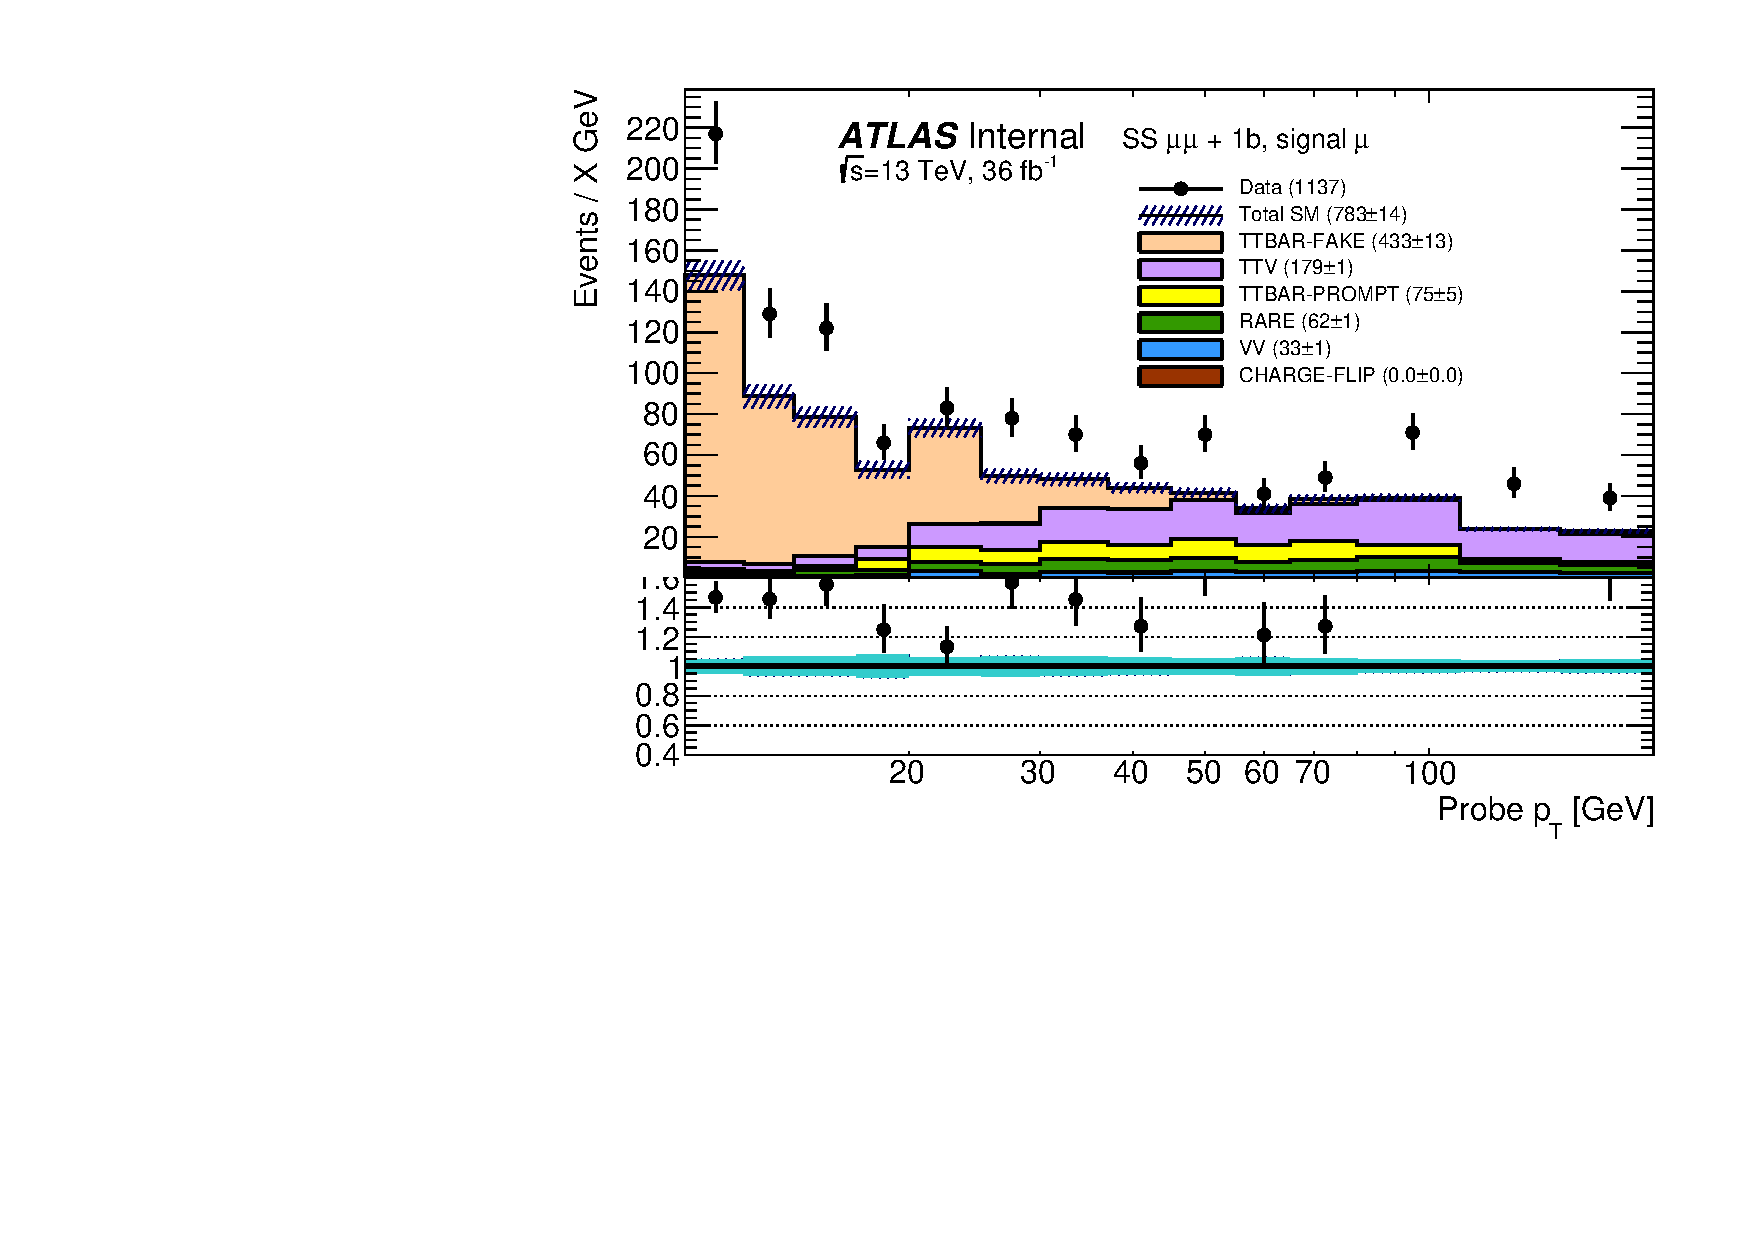
\includegraphics[width=0.49\textwidth]{INCLUSIVETAG_PROBE_PT_MUON_SIGNAL}
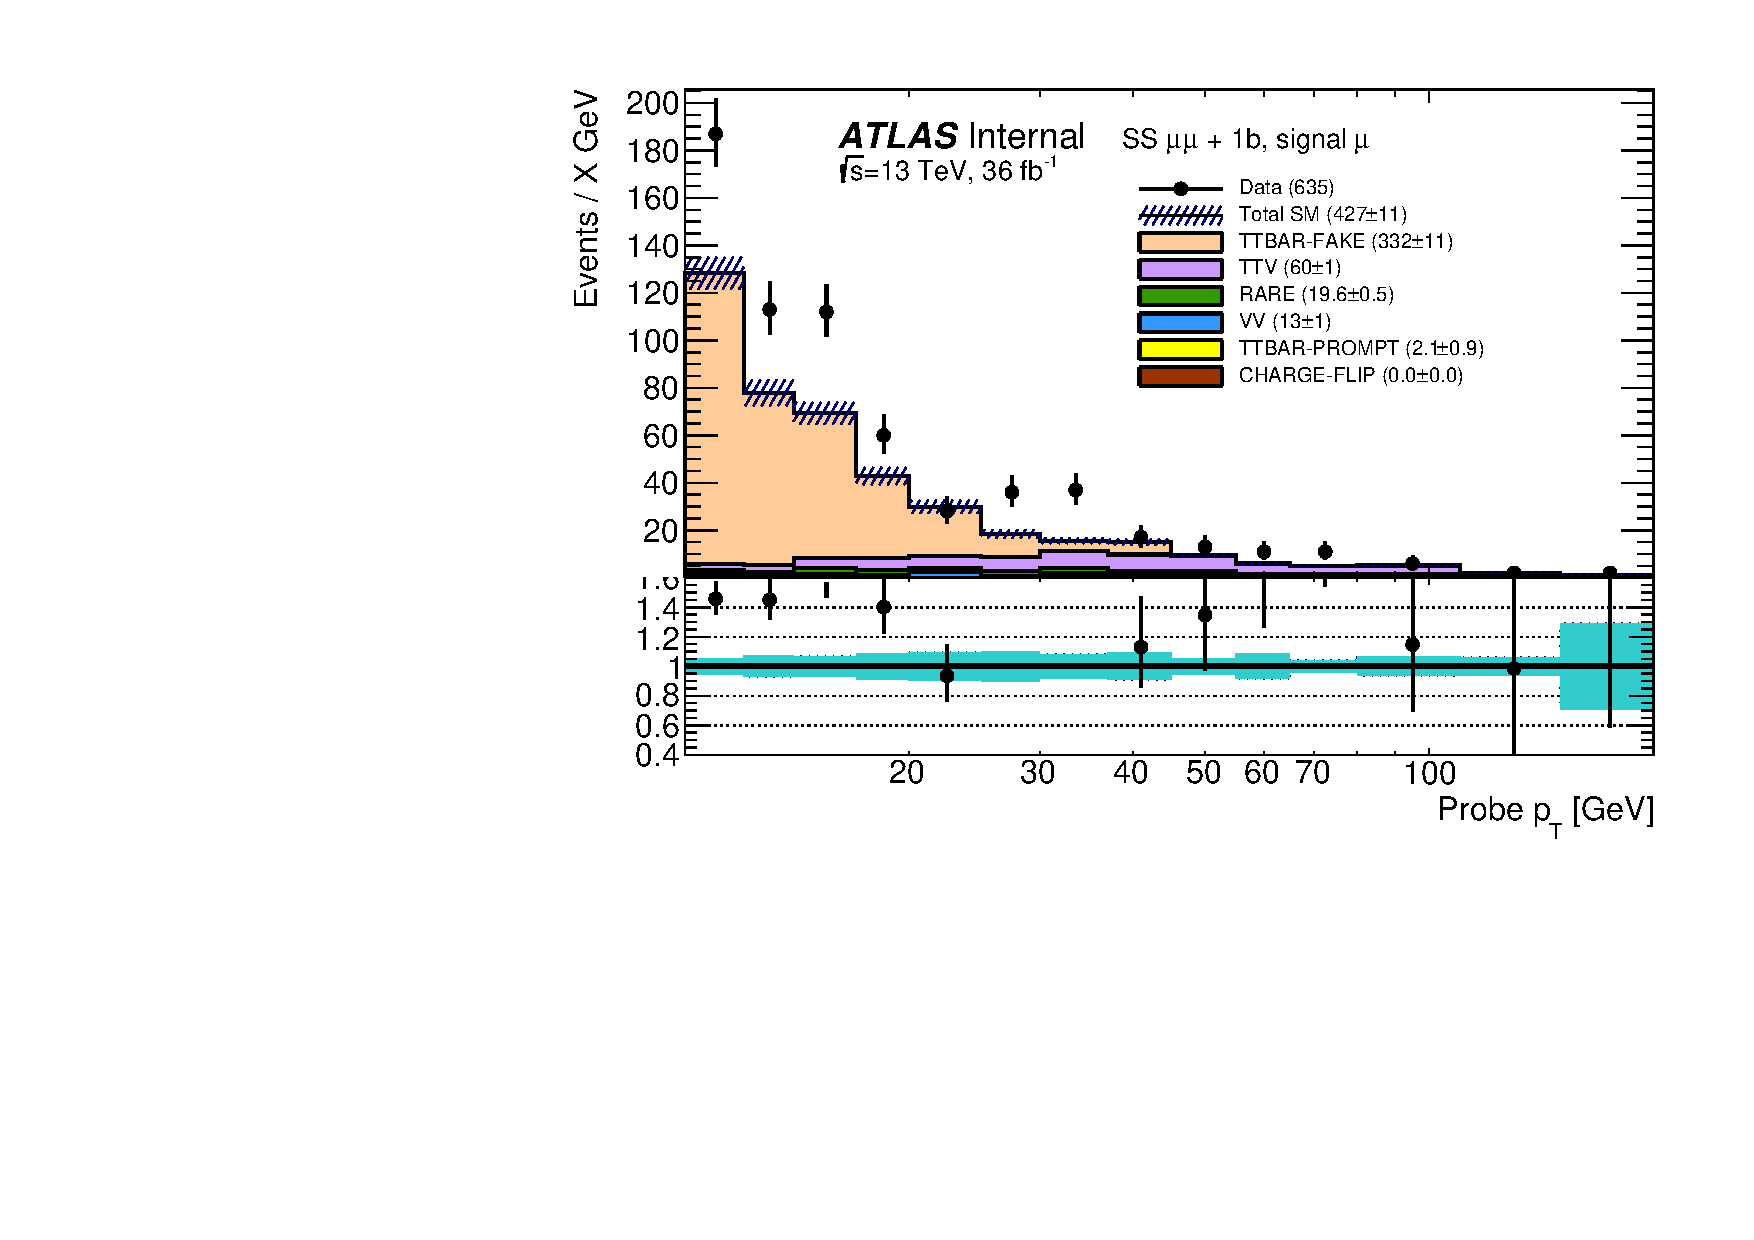
\includegraphics[width=0.49\textwidth]{IDEALTAG_PROBE_PT_MUON_SIGNAL}
\caption
{Signal probe muon \pt\ distribution in data and MC, after preselection (left) 
or further tightening of the tag muon requirements (right), 
as described in section~\ref{subsubsec:fakes_matrix_fake_rate_muons}. 
The yellow area indicates $t\bar t$ events in which the tag muon is fake and the probe real, 
leading to a measurement bias. 
}
\label{Fig:fakes_preselection_muon}
\end{figure}
%%

Figure~\ref{Fig:fakes_preselection_muon} left shows the number of signal muon probes available after this preselection. 
A similar level of disagreement between data and simulation as reported elsewhere in this document is observed, 
with data exceeding the MC predictions; this is not a concern for the purpose of this section, of course. 
One can notice that at this stage, measurements above 25 \GeV would be very affected by the important fraction of events 
in which the tag muon is fake and the probe muon is real. 
To overcome this issue, we considered three alternatives: 
\begin{itemize}
\item tighten the \pt\ and isolation requirements of the tag muon beyond those defining our usual ``signal'' category, 
to reduce its probability of being a fake muon
\item use an identical selection for tag and probe muons, and require them to be in the same (\pt,$\eta$) bin for the measurement; 
after subtraction of estimated contributions from processes with two prompt muons, all events have one real and one fake muon, 
and the symmetry in the muon selection can be taken advantage of to obtain an unbiased measurement of the fake rate: 
$$
\zeta = \frac{\varepsilon n_2}{\varepsilon n_1+(2\varepsilon-1)n_2}
$$
$\text{ with }n_1, n_2\text{ the number of events with 1 or 2 signal muons}, 
\text{ and }\varepsilon\text{ the efficiency for prompt muons.}$

This method is limited to measurements in inclusive or wide bins. 
It also can't be used at too low \pt, due to contributions from processes with two fake muons (e.g. from $B\bar B$ meson production). 
\item a generalization of the former recovering events in which the two muons may also be in different (\pt,$\eta$) bins, 
numerically solving a system of non-linear equations 
to determine simultaneously the fake rates in different bins in an unbiased way. 
Upgraded from asymptotic equalities to statistical estimates, 
this was in fact implemented as the maximization of a likelihood built from a product of multinomial PDFs. 
\end{itemize}
Details on the implementation and performances of these three methods are provided in appendix~\ref{app:fake_rates}. 
Comparisons made with $t\bar t$ MC indicated that when using a very tight isolation requirement on the tag muon 
($\operatorname{max}(E_\mathrm{T}^\text{topo, cone 40},p_\mathrm{T}^\text{cone 40})<0.02\times\pt$), 
the level of bias is always largely inferior to the statistical uncertainty in the measurement, 
which itself is smaller than for the other two methods. 

Figure~\ref{Fig:fakes_preselection_muon} right shows the number of signal muon probes when applying those reinforced isolation criteria to the tag muon, 
as well as requiring $p_\mathrm{T}^\text{tag}>\operatorname{max}(40,p_\mathrm{T}^\text{probe}+10)$ GeV. 
As expected, the number of pairs with a fake tag muons is down to a minor level, at least according to the simulation. 
Similar distributions for baseline probe muons can be found in appendix~\ref{app:fake_rates}. 

%%
\begin{figure}[t!]
\centering
\includegraphics[width=0.49\textwidth]{{TTBAR.Incl.FakeRate.Muon}.pdf}
\includegraphics[width=0.49\textwidth]{{TTBAR.Incl.FakeRateVsEta.Muon}.pdf}
\caption
{
Muon fake rates in $t\bar t$ MC with an inclusive selection, 
as function of \pt\ (left, green markers) or $|\eta|$ in different momentum ranges (right). 
}
\label{Fig:fakes_MC_inclusive_rates_muon}
\end{figure}
%%

Muon fake rates as predicted by the simulation ($t\bar t$, inclusive selection of leptons via truth-matching) 
are shown on Fig.~\ref{Fig:fakes_MC_inclusive_rates_muon} as function of \pt\ and $|\eta|$. 
One can expect a moderate dependency of the fake rates to the transverse momentum, with the strongest evolution at low \pt and a slight increase toward higher \pt. 
The fake rates are also essentially independent of the pseudorapidity, 
except at the edge ($|\eta|>2.3$) where there is a strongly pronounced increase of the rates. 
This motivates measurements in data as function of \pt\ in two $|\eta|$ bins. 

Observations in data seem to indicate that the rejection of fake tag muons by the reinforced isolation criteria 
is quite less important than in the simulation, or that the amount of fake muons at high \pt\ is larger than in the simulation, or both. 
This leads to an unknown level of bias in measurements performed with the straightforward tag-and-probe selection at high \pt. 
For that reason, the final rates measured in data are provided by the tag-and-probe method below 25 \GeV, 
and by the symmetric selection for $\pt>25 \GeV$. The former are obtained with 

\begin{align}
\zeta&=\frac{n_\text{signal}^\text{data} - n_\text{signal}^\text{MC}}{n_\text{baseline}^\text{data} - n_\text{baseline}^\text{MC}}\\
\text{with }&\Delta\zeta_\text{stat} = \frac{\sqrt{(1-2\zeta)n_\text{signal}^\text{data} + \zeta^2 n_\text{baseline}^\text{data}}}
{n_\text{baseline}^\text{data} - n_\text{baseline}^\text{MC}}\notag
%\text{and }&\Delta\zeta_\text{syst} = \frac{\Delta B}{B}\times\frac{\sqrt{(1-\zeta^2)(n_\text{signal}^\text{MC})^2 
%+ \zeta^2 (n_\text{baseline}^\text{MC} - n_\text{signal}^\text{MC})^2 }}
\end{align}
while the latter are obtained with:
\begin{align}
\zeta &= \frac{\varepsilon (n_\text{both signal}^\text{data} - n_\text{both signal}^\text{MC})}
{\varepsilon (n_\text{only 1 signal}^\text{data} - n_\text{only 1 signal}^\text{MC})
+(2\varepsilon-1)(n_\text{both signal}^\text{data} - n_\text{both signal}^\text{MC})}\\
\text{with }&\Delta\zeta_\text{stat} 
= \frac{\zeta}{n_\text{both signal}^\text{data} - n_\text{both signal}^\text{MC}}
\sqrt{\zeta^2 n_\text{only 1 signal} + \left(1-\frac{2\varepsilon-1}{\varepsilon}\zeta\right)^2 n_\text{both signal}}\notag
\end{align}
the efficiency for prompt muons $\varepsilon$ is assigned values compatible with section~\ref{subsubsec:fakes_matrix_real_efficiency}. 

The measured rates are presented in Table~\ref{table:fake_rates_muon}. 
The central values are shown together with the associated statistical uncertainty, 
as well as the propagation of the uncertainty on the subtracted backgrounds normalization, 
which is taken as a global $\Delta B/B=20\%$. 
The rates are of the order of $10\%$ up to 30 GeV, beyond which they increase. 
Overall these values are not very different from those predicted by the simulation. 

Complementary information (event yields for data and background processes, estimates of the level of bias and contributions from QCD double-fakes) 
can be found in appendix~\ref{app:fake_rates}. 
The observed rates are quite in agreement with the simulation up to $\pt\sim 50\GeV$. 

%%
\begin{table}[t!]
\def\arraystretch{1.15}
\caption{Muon fake rate measured in data and the associated statistical uncertainty. 
The systematic uncertainty originating from the subtraction of ``backgrounds'' with only prompt leptons is also displayed. }
\label{table:fake_rates_muon}
\def\arraystretch{1.15}
\centering
\resizebox{\textwidth}{!}{
\begin{tabular}{|c|c|c|c|} \hline\hline
\multicolumn{2}{|c|}{$10<\pt<12 \GeV$}         & \multicolumn{2}{c|}{$12<\pt<14$}                  \\   
$|\eta|<2.3$             & $|\eta|>2.3$             & $|\eta|<2.3$             & $|\eta|>2.3$            \\
$0.14 \pm 0.01 \pm 0.00$ & $0.22 \pm 0.05 \pm 0.00$ & $0.11 \pm 0.01 \pm 0.00$ & $0.24 \pm 0.06 \pm 0.00$ \\ 
\hline \hline
\end{tabular}}

\resizebox{\textwidth}{!}{
\begin{tabular}{|c|c|c|c|} \hline\hline
\multicolumn{2}{|c|}{$14<\pt<17$}                    & \multicolumn{2}{c|}{$17<\pt< 20 \GeV$}       \\       
$|\eta|<2.3$             & $|\eta|>2.3$             & $|\eta|<2.3$             & $|\eta|>2.3$            \\    
$0.12 \pm 0.01 \pm 0.00$ & $0.09 \pm 0.05 \pm 0.00$ & $0.09 \pm 0.01 \pm 0.00$ & $0.21 \pm 0.07 \pm 0.00$ \\
\hline \hline
\end{tabular}}

\resizebox{\textwidth}{!}{
\begin{tabular}{|c|c|c|c|c|} \hline\hline
             $20<\pt<30$ &              $30<\pt<40$ &              $40<\pt<60$ &                $\pt>60$ \\
$0.07 \pm 0.02 \pm 0.00$ & $0.12 \pm 0.05 \pm 0.01$ & $0.16 \pm 0.09 \pm 0.04$ & $0.49 \pm 0.10 \pm 0.07$ \\
\hline \hline
\end{tabular}}

\end{table}

Some of the validation and signal regions require events with 2 or more $b$-tagged jets, 
which reduces the fraction of non-prompt muons coming from $B$ meson decays. 
Figure~\ref{fig:fakes_MC_vsBjets_muon} illustrates how this impacts on the fake rates. 
Given the good agreement between data and simulation for the measured values, 
we chose to apply a correction to the measured rates for events with $\ge 2$ $b$-jets, 
taken directly from simulated $t\bar t$ events. 
This correction factor varies between 1 and 2 with \pt, 
and the whole size of the correction is assigned as an additional systematic uncertainty (see Table~\ref{tab:fake_rates_muon_systematics}). 

\begin{table}[t!]
\def\arraystretch{1.15}
\caption{Additional systematic uncertainty on the muon fake rates, to address variations of the latter in different environments. 
The table also shows the correction factors and uncertainties applied to final states with $\ge 2$ $b$-tagged jets.}
\label{tab:fake_rates_muon_systematics}
\def\arraystretch{1.15}
\centering
\resizebox{\textwidth}{!}{
\begin{tabular}{|c|c|c|c|c|c|c|} \hline\hline
 \pt & $<14$ & $14-20$ & $20-30$ & $30-40$ & $40-60$ & $>60$\\\hline
$\Delta\zeta^\text{(syst)}$ & 30\% & 30\%  & 30\%     &  50\%   & \multicolumn{2}{c|}{
		\begin{tabular}{@{}c@{}}50\% for $H_\mathrm{T}<600$ \\ 70\% for $600<H_\mathrm{T}<1200$ \\85\% for $H_\mathrm{T}>1200$\end{tabular}} \\\hline
$\frac{\zeta_{\ge 2b}}{\zeta}$ & $1.2\pm 0.2$ & $1.5\pm 0.5$ & $1.7\pm 0.7$ & $2.0\pm 1.0$ & $1.5\pm 0.5$ & $-$\\\hline
\end{tabular}}
\end{table}


%%
\par{\bf Systematic uncertainties\\}
To cover potential differences in the fake rates between the measurement regions and the signal regions, 
that could be due to different origins or kinematic properties of the fake leptons, 
uncertainties are set based on the extent of those differences predicted by the simulation. 
The largest effect is the decrease of the fake rates with $H\mathrm{T}$ (especially for high-\pt\ muons), 
which likely correlates to a harder jet at the origin of the non-prompt muon, hence a reduced likelihood to satisfy isolation requirements. 
Details can be consulted in appendix~\ref{app:fake_rates}, 
and Table~\ref{tab:fake_rates_muon_systematics} summarizes the additional systematic uncertainties applied to the muon fake rates. 
They vary from $30\%$ at low \pt, to up to 85\% for $\pt>40 \GeV$; in that range, the uncertainties are made $H_\mathrm{T}$-dependent. 

As already shown, Fig.~\ref{fig:fakes_MC_vsBjets_muon} shows the variation of the fake rate in $t\bar t$ MC as function of the number of $b$-tagged jets in the event. 
Unsurprisingly, the rates are very similar for $0b$ and $\ge 1b$ final states, 
justifying the use of the fake rates measured in this section (i.e. in a $\ge 1b$ region) to predict fake muon background in all signal regions. 

\begin{figure}[t!]
\centering
\includegraphics[width=0.49\textwidth]{{TTBAR.BjetImpact.FakeRate.Muon}.pdf}
\caption
{
Muon fake rates in $t\bar t$ MC with an inclusive selection, 
as function of \pt\ and split according to the number of $b$-tagged jets in the event. 
}
\label{fig:fakes_MC_vsBjets_muon}
\end{figure}

\subsection{Baseline-to-signal efficiency for fake electrons}
\label{subsubsec:fakes_matrix_fake_rate_electrons}


%%
\begin{figure}[t!]
\centering
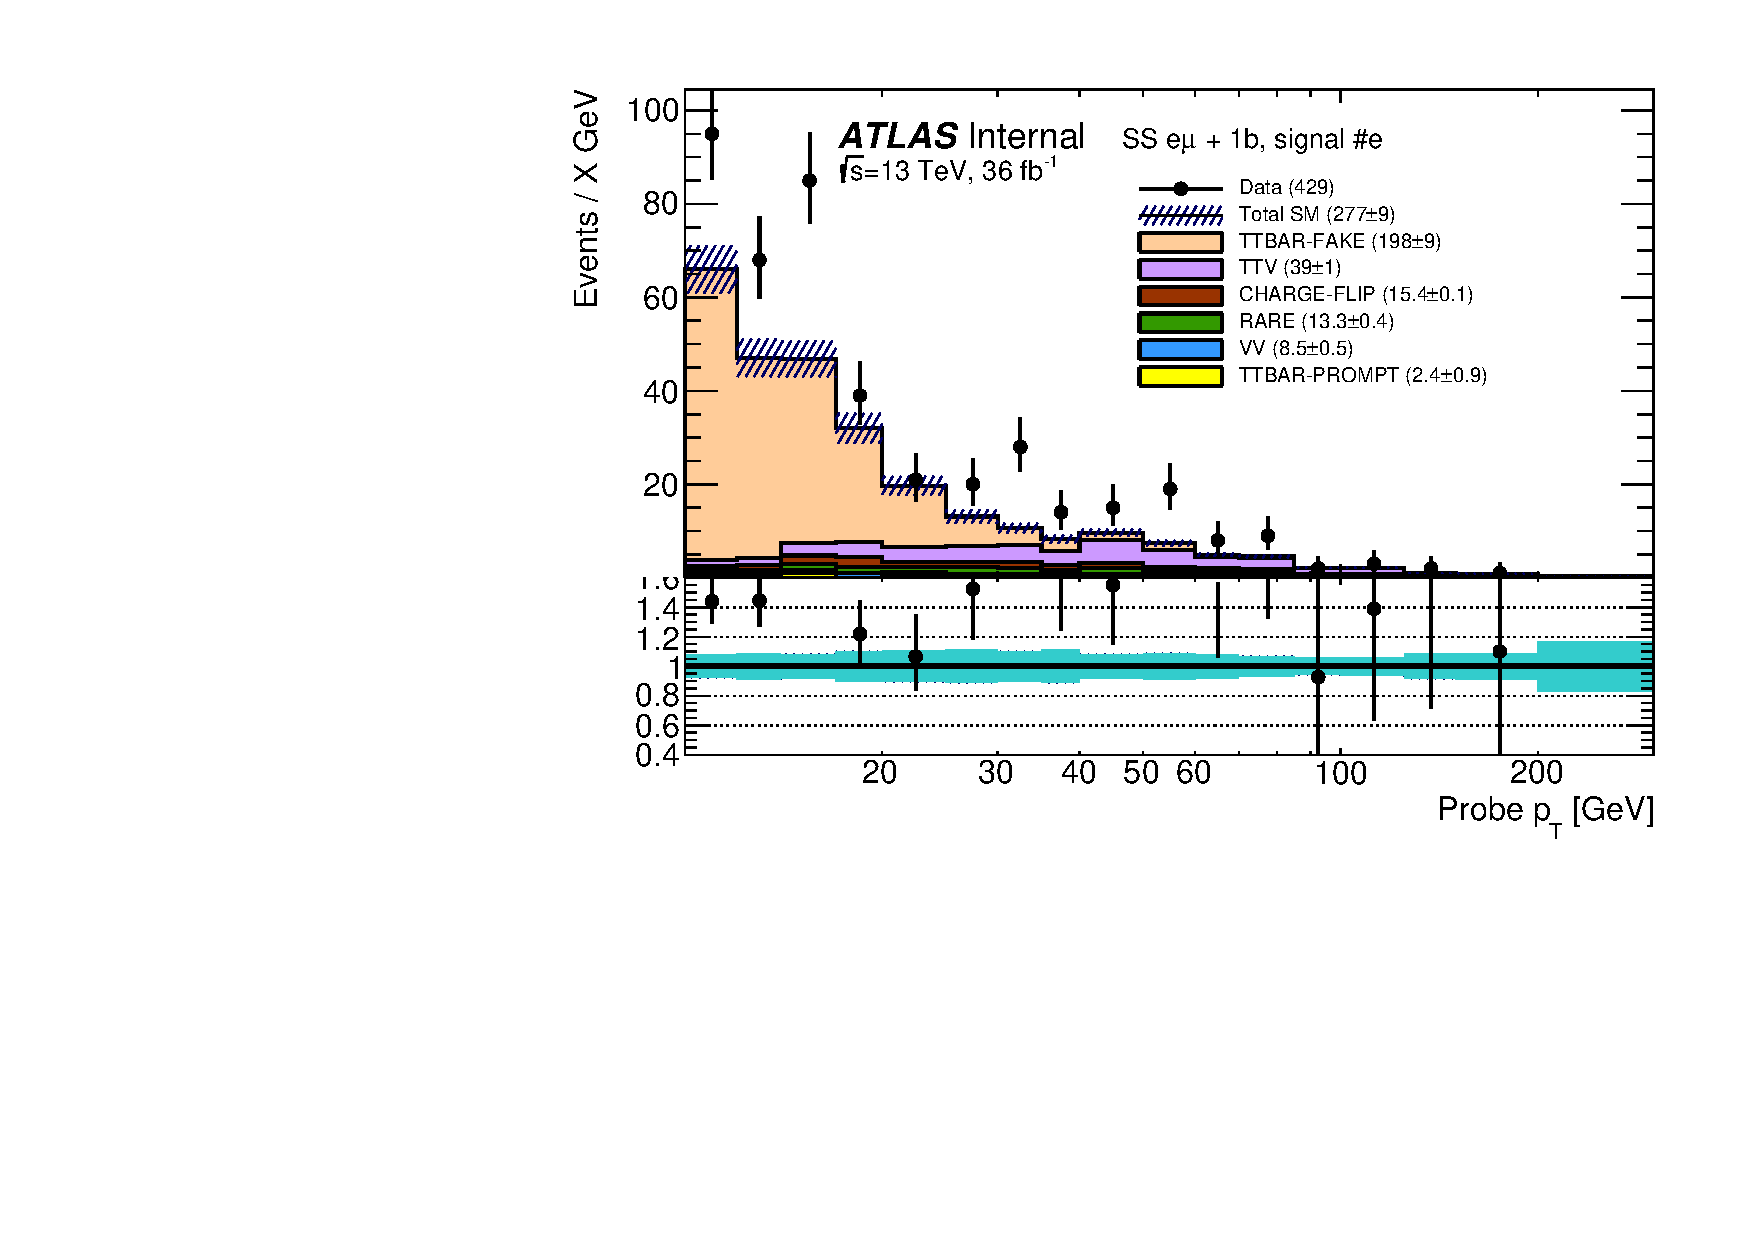
\includegraphics[width=0.49\textwidth]{IDEALTAG_CFTPROBE_PT_ELECTRON_SIGNAL}
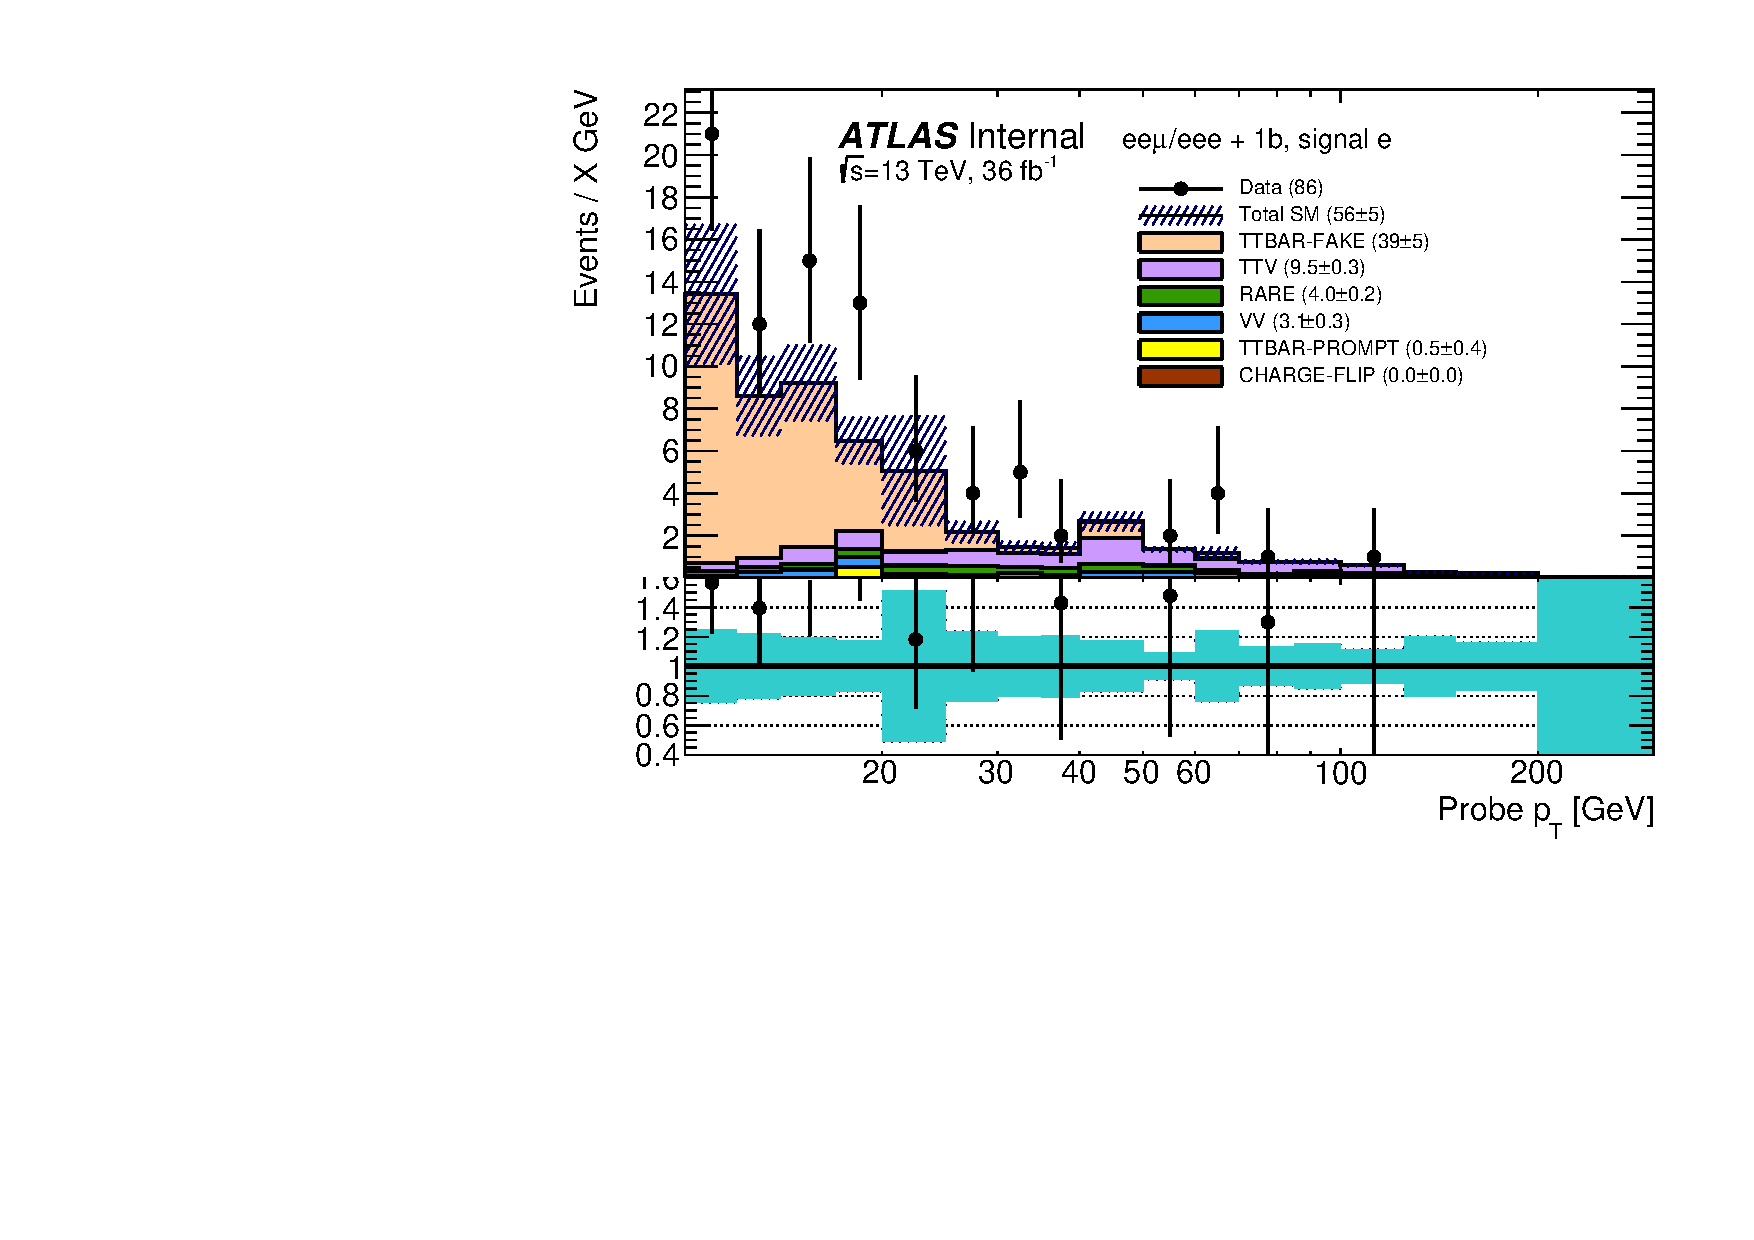
\includegraphics[width=0.49\textwidth]{TRILEP_IDEALTAG_PROBE_PT_ELECTRON_SIGNAL}
\caption
{Signal probe electron \pt\ distribution in data and MC, for $e^\pm\mu^\pm$ pairs (left, with probe electrons satisfying CFT cut and a reinforced tag muon selection) 
or $\ell^\pm e^\mp e^\mp$ pairs (right, with reinforced tag electron selection), 
as described in section~\ref{subsubsec:fakes_matrix_fake_rate_electrons}. 
The yellow area indicates $t\bar t$ events in which the tag lepton is fake and the probe electron real, 
leading to a measurement bias. 
}
\label{Fig:fakes_preselection_electron}
\end{figure}
%%

Electron fake rates are measured with a similar methodology, but the $e^\pm e^\pm$ channel is unusable to the presence of a large charge-flip background. 
This is overcome by working with $e^\pm\mu^\pm$ pairs instead (with a tag muon), but mixing leptons of different flavours brings additional complications 
(one can not, for example, use the unbiased measurement employed to measure muon fakes rates at higher \pt, as there is no symmetry between the leptons). 
To improve confidence, measurements are performed in four different ways, which complement each other: 
\begin{itemize}
\item straightforward tag-and-probe wit $e\mu$ pairs, with the same tag muon selection as in the previous section. 
\item same selection, but subtracting from the numerator the number of pairs with one fake tag muon and one prompt probe electron, 
itself estimated from the number of observed $e\mu$ events with a muon failing signal requirements, 
scaled by a ``muon fake rate'' taken as the ratio between $\mu\mu$ pairs with two or only one signal muon. 
scaled by an efficiency correction factor $e\mu/\mu\mu$ taken from $t\bar t$ MC (only for pairs with one fake muon). 
This only works if the two muons satisfy the same kinematic requirements, therefore can be used only for measurements in wide or inclusive bins. 
\item selecting $\ell^\mp e^\pm e^\pm+\ge 1b$ events, with a $Z$ veto on SFOS pairs. 
This selection entirely suppresses contributions from charge-flip, or events with fake muons. 
One of the electron, with standard signal requirements, is required to satisfy the same reinforced \pt\ and isolation requirements as for the muon measurement 
(section~\ref{subsubsec:fakes_matrix_fake_rate_muons}), 
and the measurement can be performed on the other electron. 
\item same selection, using the symmetry between the two same-sign electrons to measure the rates in an unbiased way, similarly to the muon case. 
\end{itemize}
Events are acquired with the combination of single-muon (as in previous section) and $e\mu$ triggers. 


Figure~\ref{Fig:fakes_preselection_electron} shows the number of signal probe electrons selected in the $e\mu$ and $\ell ee$ channels. 
There are quite less events selected in the trilepton channel. 
Figure~\ref{Fig:fakes_MC_inclusive_rates_electron} shows the electron fake rate as a function of \pt\ or $\eta$ in $t\bar t$ MC. 
The variations of the rates as function of the pseudorapidity are not very large, 
therefore we only perform measurements as function of \pt. 
The low \pt\ range is dominated by non-prompt electrons from heavy flavour decays, while beyond 30 \GeV, 
electron fakes mostly come from conversions of photons produced inside jets, such as $\pi^0\to\gamma\gamma$ decays (see appendix). 

%%
\begin{figure}[t!]
\centering
\includegraphics[width=0.49\textwidth]{{TTBAR.Incl.FakeRate.Electron}.pdf}
\includegraphics[width=0.49\textwidth]{{TTBAR.Incl.FakeRateVsEta.Electron}.pdf}
\caption
{
Electron fake rates in $t\bar t$ MC with an inclusive selection, 
as function of \pt\ (left, yellow/green markers = with/without CFT cut applied) or $|\eta|$ in different momentum ranges (right). 
}
\label{Fig:fakes_MC_inclusive_rates_electron}
\end{figure}
%%

Based on the estimated levels of bias, and achievable statistical precision, of the different methods, 
we decided to measure electron fake rates with the tag-and-probe $e\mu$ selection up to 30 \GeV, 
and by combining ``unbiased'' evaluations in both $e\mu$ and $\ell ee$ channels beyond. 
The measured rates are presented in Table~\ref{table:fake_rates_electron}, 
together with the associated statistical and background-subtraction uncertainties. 
The rates are here as well of the order of $10\%$ up to 30 GeV, beyond which they increase to up to 25\%. 

%%
\begin{table}[t!]
\def\arraystretch{1.15}
\caption{Electron fake rate measured in data and the associated statistical uncertainty. 
The systematic uncertainty originating from the subtraction of ``backgrounds'' with only prompt leptons is also displayed. }
\label{table:fake_rates_electron}
\def\arraystretch{1.15}
\centering
\resizebox{\textwidth}{!}{
\begin{tabular}{|c|c|c|c|} \hline\hline
             $10<\pt<12$ &              $12<\pt<14$ &              $14<\pt<17$ &             $17<\pt<20$ \\
$0.10 \pm 0.01 \pm 0.00$ & $0.10 \pm 0.01 \pm 0.01$ & $0.12 \pm 0.01 \pm 0.01$ & $0.08 \pm 0.02 \pm 0.00$ \\
\hline \hline
\end{tabular}}

\resizebox{\textwidth}{!}{
\begin{tabular}{|c|c|c|c|} \hline\hline
             $20<\pt<25$ &              $25<\pt<30$ &              $30<\pt<40$ &             $40>\pt$ \\
$0.07 \pm 0.02 \pm 0.01$ & $0.11 \pm 0.03 \pm 0.01$ & $0.20 \pm 0.07 \pm 0.03$ & $0.25 \pm 0.10 \pm 0.05$ \\
\hline \hline
\end{tabular}}

\end{table}

Unlike muons, we do not so far apply MC-based correction factors for final states with $\ge 2$ $b$-tagged jets. 
This is because there is less good agreement between the measured rates and the simulation; 
in particular the former take larger values in the medium-\pt\ range. 

%%
\par{\bf Systematic uncertainties\\}

Similarly to the muon case, systematic uncertainties are assigned to cover for difference in the rates in the measurement regions in the signal regions, 
that would be due to different sources of fake leptons, or different kinematic properties of these sources. 

Details can be consulted in appendix~\ref{app:fake_rates}. Unlike muons, there is much less of a dependency to $H_\mathrm{T}$. 
The dominant source of potential differences is therefore the origin of the fake electron (see Fig.~\ref{fig:fakes_MC_perSource_electron}); 
for $\pt<20 \GeV$, non-prompt electrons from HF hadron decays dominate with some certainty, 
which is confirmed by the good agreement between MC fake rates and those measured in data. 
In that range, we assign a $30\%$ uncertainty on the fake rates (inflated to $50\%$ for final states with $\ge 2b$-tagged jets). Beyond, the rates measured in data are larger than those predicted by the simulation, 
and would for example be consistent with a larger amount of electrons from photon conversions than predicted. 
In that range, we therefore assign a $50\%$ uncertainty, which covers any arbitrary variation of the relative contributions of each source. 

Finally, Figure~\ref{fig:fakes_MC_vsBjets_electron} shows the variation of the fake rate in $t\bar t$ MC as function of the number of $b$-tagged jets in the event. 
Unsurprisingly, the rates are very similar for $0b$ and $\ge 1b$ final states, 
justifying the use of the fake rates measured in this section (i.e. in a $\ge 1b$ region) to predict fake electron background in all signal regions. 
We do not assign extra uncertainties for final states with $\ge 2b$-jets for $\pt>20$ GeV: if, indeed, the relative contribution of HF decays is smaller than expected in that range, 
then there should be less intrinsic difference between $0/1b$ and $\ge 2b$ final states, and those are already within the existing uncertainties. 

\begin{figure}[t!]
\centering
\includegraphics[width=0.49\textwidth]{{TTBAR.Incl.FakeRate.PerSource.Electron}.pdf}
\includegraphics[width=0.49\textwidth]{{TTBAR.BjetImpact.FakeRate.Electron}.pdf}
\caption
{
Electron fake rates in $t\bar t$ MC with an inclusive selection, 
as function of \pt\ and split according to the source of the fake electron (left). 
The relative contributions of each source (for signal electrons) are indicated on the right-hand-side. 
}
\label{fig:fakes_MC_perSource_electron}
\end{figure}


\begin{figure}[t!]
\centering
\includegraphics[width=0.49\textwidth]{{TTBAR.Incl.FakeRate.PerSource.Electron}.pdf}
\includegraphics[width=0.49\textwidth]{{TTBAR.BjetImpact.FakeRate.Electron}.pdf}
\caption
{
Electron fake rates in $t\bar t$ MC with an inclusive selection, 
as function of \pt\ and split according to the number of $b$-tagged jets in the event.  
}
\label{fig:fakes_MC_vsBjets_electron}
\end{figure}


\subsection{Baseline-to-signal efficiency for real leptons}
\label{subsubsec:fakes_matrix_real_efficiency}

% mostly copy-pasted from 2015 supporting note

Baseline-to-signal efficiency for real leptons is measured in a high purity data sample of opposite-sign same-flavor leptons with the standard $Z$ tag-and-probe method.
Events are selected by a single lepton trigger,  
\texttt{e24\_lhmedium\_iloose\_L1EM20VH}  or \texttt{e26\_lhtight\_nod0\_ivarloose} for electrons,
\texttt{mu20\_iloose\_L1MU15} or \texttt{mu26\_ivarmedium} for muons,
respectively in 2015 or 2016 data. 
The tag lepton, required to have triggered the event recording, also satisfies signal requirements and verifies $\pt>25 \GeV$. 
The probe lepton used for the efficiency measurement satisfies baseline requirements. 
All possible tag-and-probe combinations are considered in an event (including permutation of the tag and probe leptons), 
as long as the invariant mass of the pair is comprised between 80 and 100 \GeV. 
Figure~\ref{fig:RLE_mll_distribution} illustrates this event selection.

\begin{figure}[t!]
\centering
\begin{subfigure}[b]{0.45\textwidth}
	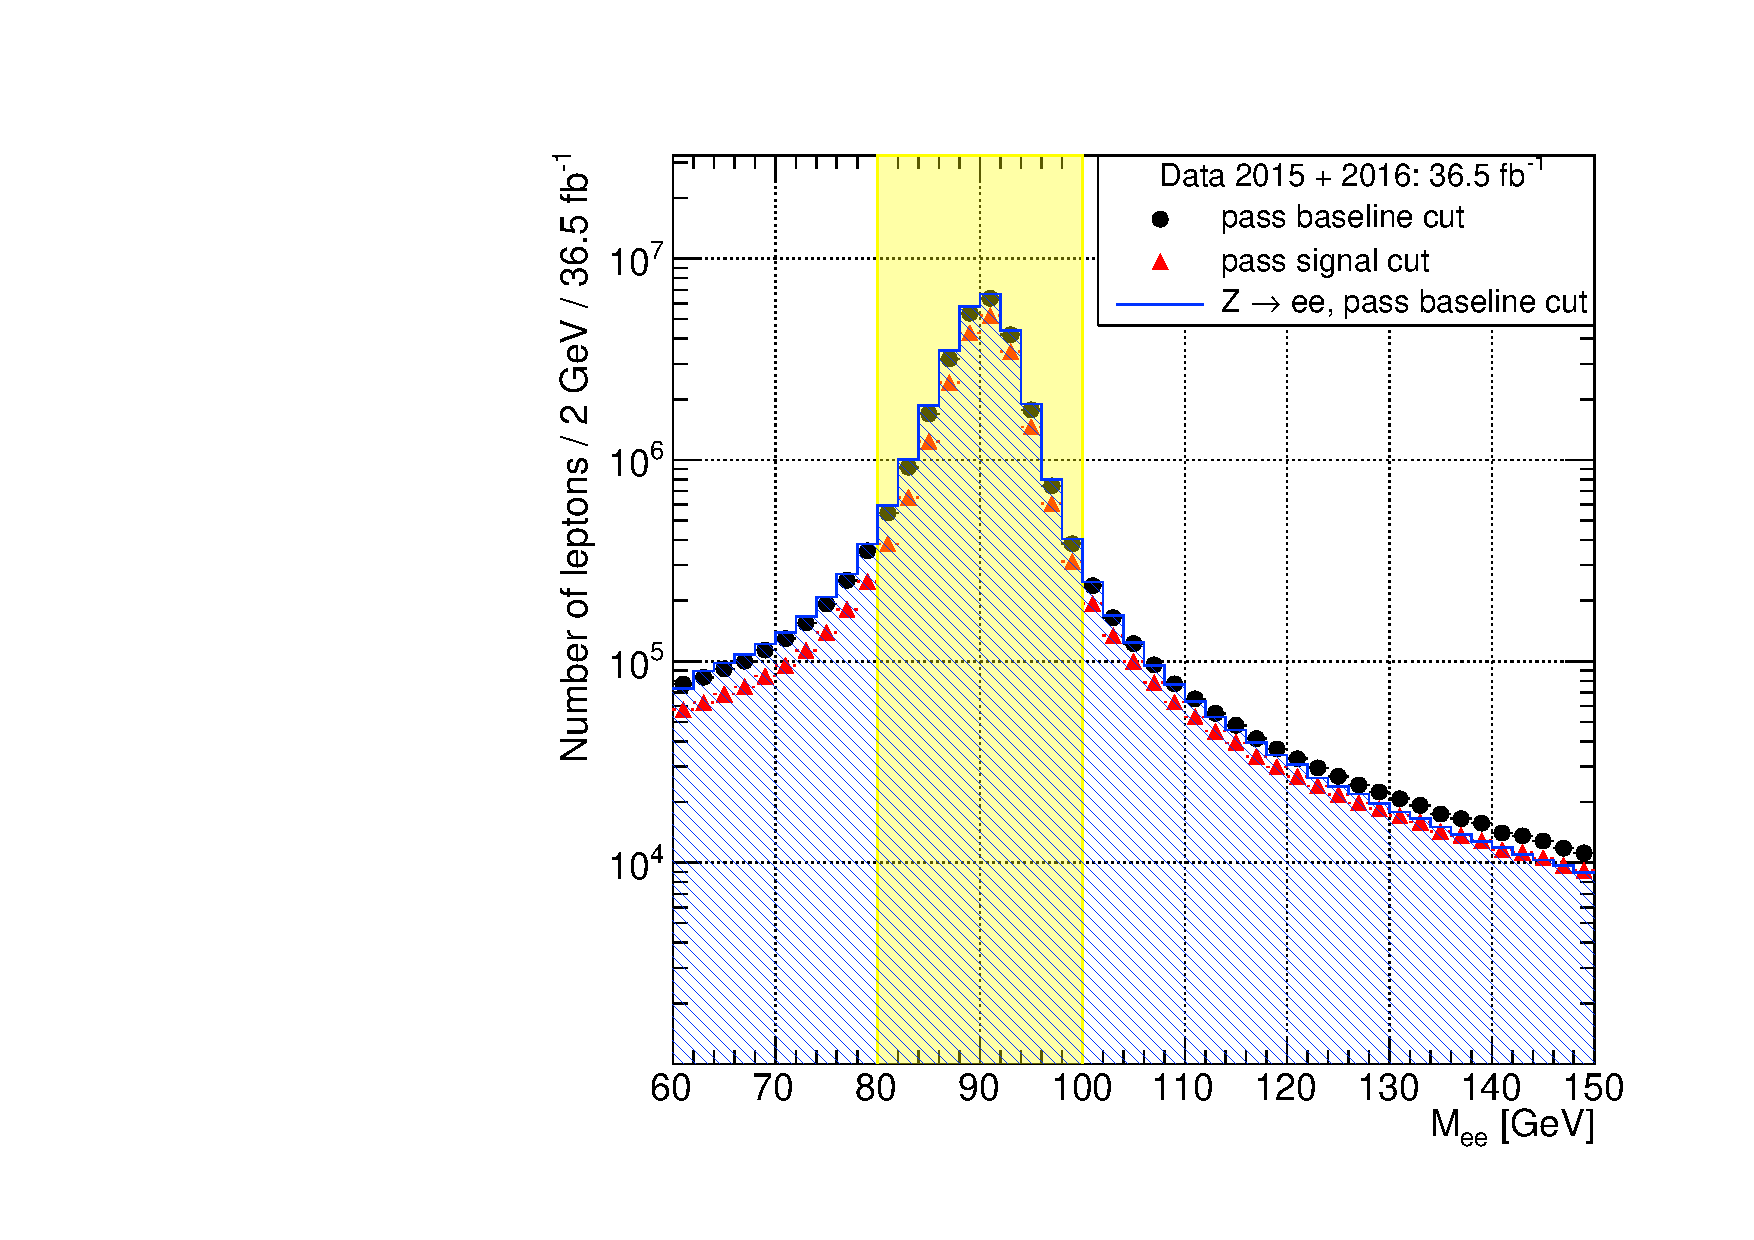
\includegraphics[width=\textwidth]{baseline_and_signal_mll_distribution_Mee.pdf}
\end{subfigure}
\begin{subfigure}[b]{0.45\textwidth}
	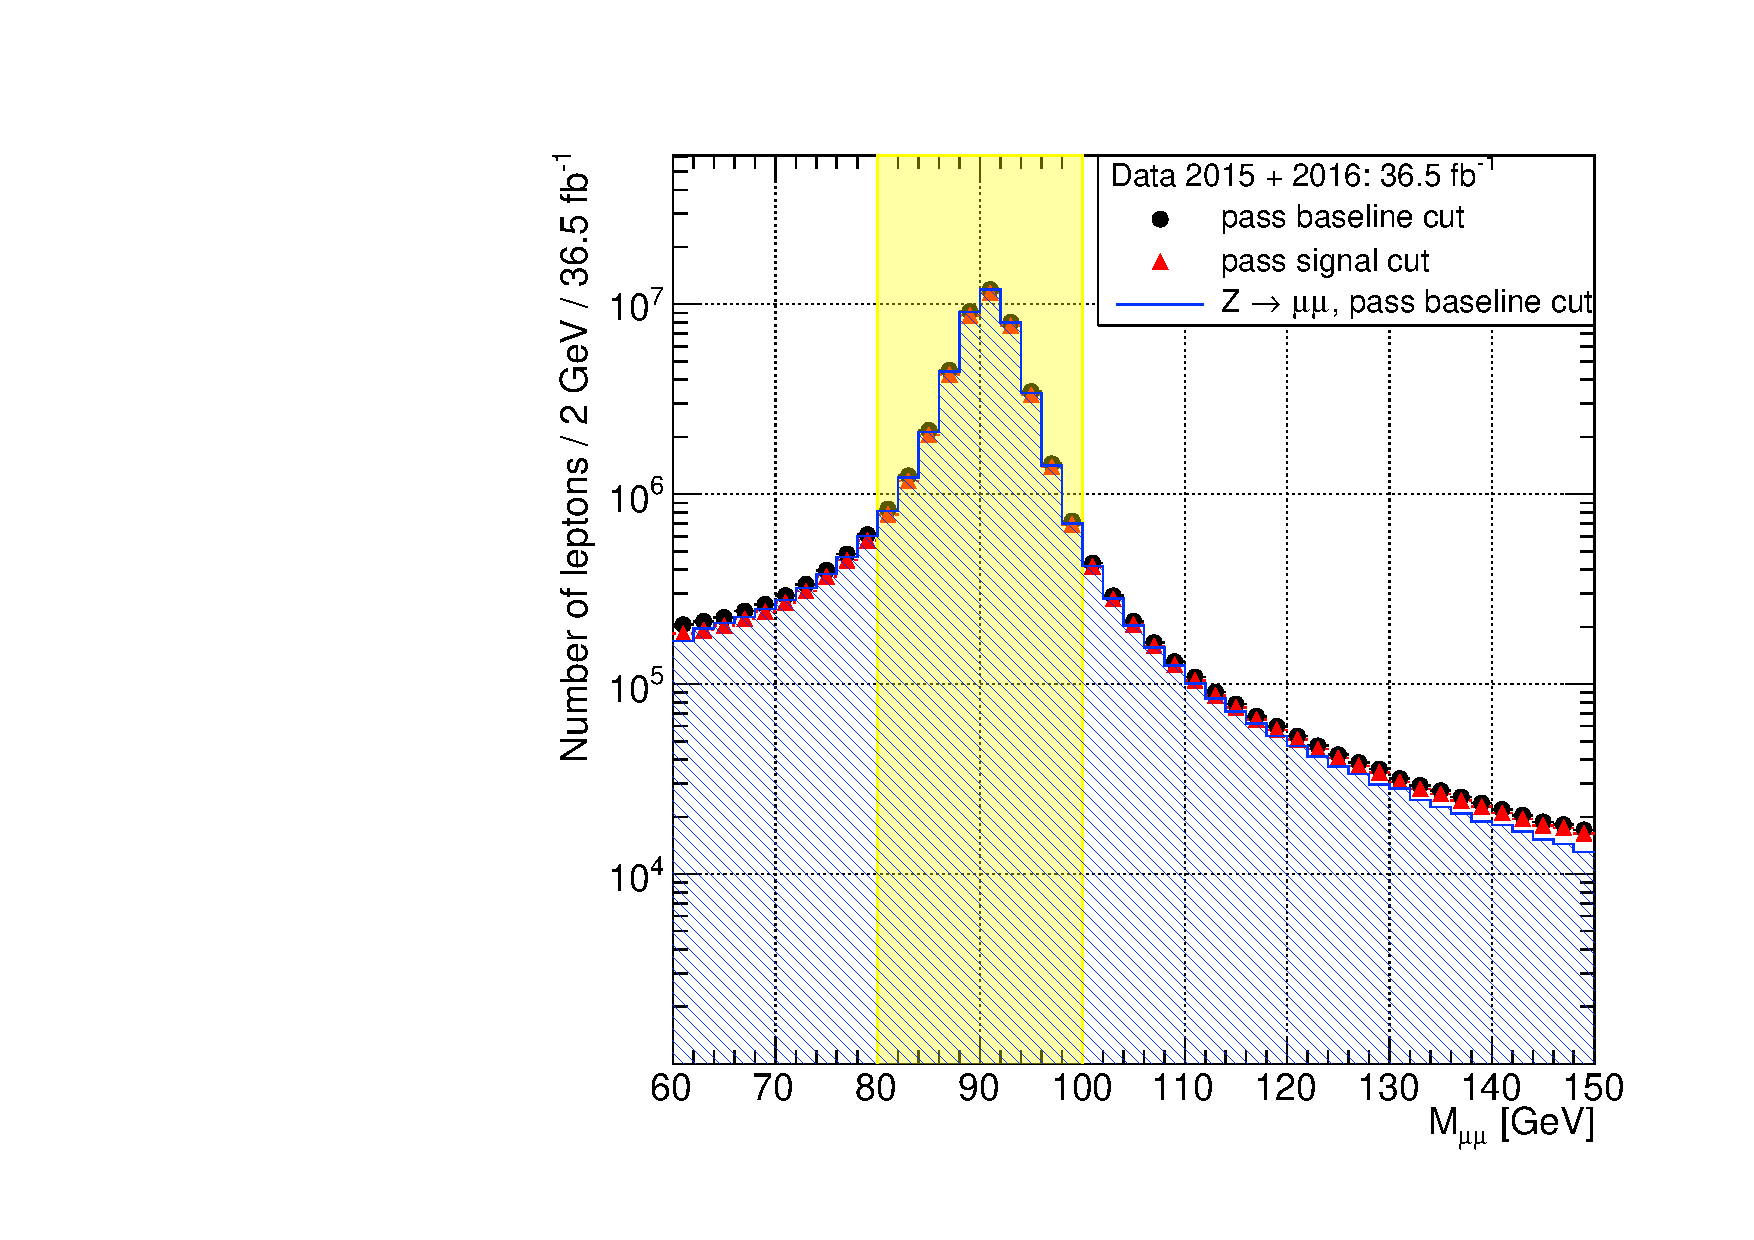
\includegraphics[width=\textwidth]{baseline_and_signal_mll_distribution_Mmumu.pdf}
\end{subfigure}
\caption{Invariant mass of opposite-sign same-flavor electrons (left) and muons (right), after the tag selection, 
where the probe satisfies the baseline requirements or the signal requirements.}
\label{fig:RLE_mll_distribution}
\end{figure}

A non-negligible background contamination in the electron channel affects measurements below $\pt=20 \GeV$. 
This contamination is taken into account in the measurement using a background template method inspired by the one used by the $e/\gamma$ CP group to measure reconstruction, identification, and isolation efficiencies~\cite{ATLAS-CONF-2014-032}. 
This template is built from the tag-and-probe invariant mass distribution for baseline-level probe electrons that fail both tighter PID cuts (\texttt{mediumLH}) and isolation requirements, smoothed by assuming an exponential shape whose parameters are determined by a fit in the interval $60<m_{ee}<120 \GeV$ excluding the $80<m_{ee}< 100 \GeV$ region. 
The background template is then normalized to the main tag-and-probe distribution in the background-dominated tail $120<m_{ee}<150 \GeV$. 
More details and validation of the method will be provided in the appendix~\ref{app:real_lepton_efficiency}. 
The estimated level of background goes up to $4\%$, reached for probe electrons with $\pt<15 \GeV$ and $|\eta|<0.8$. 

\begin{figure}[t!]
\centering
\begin{subfigure}{0.49\textwidth}
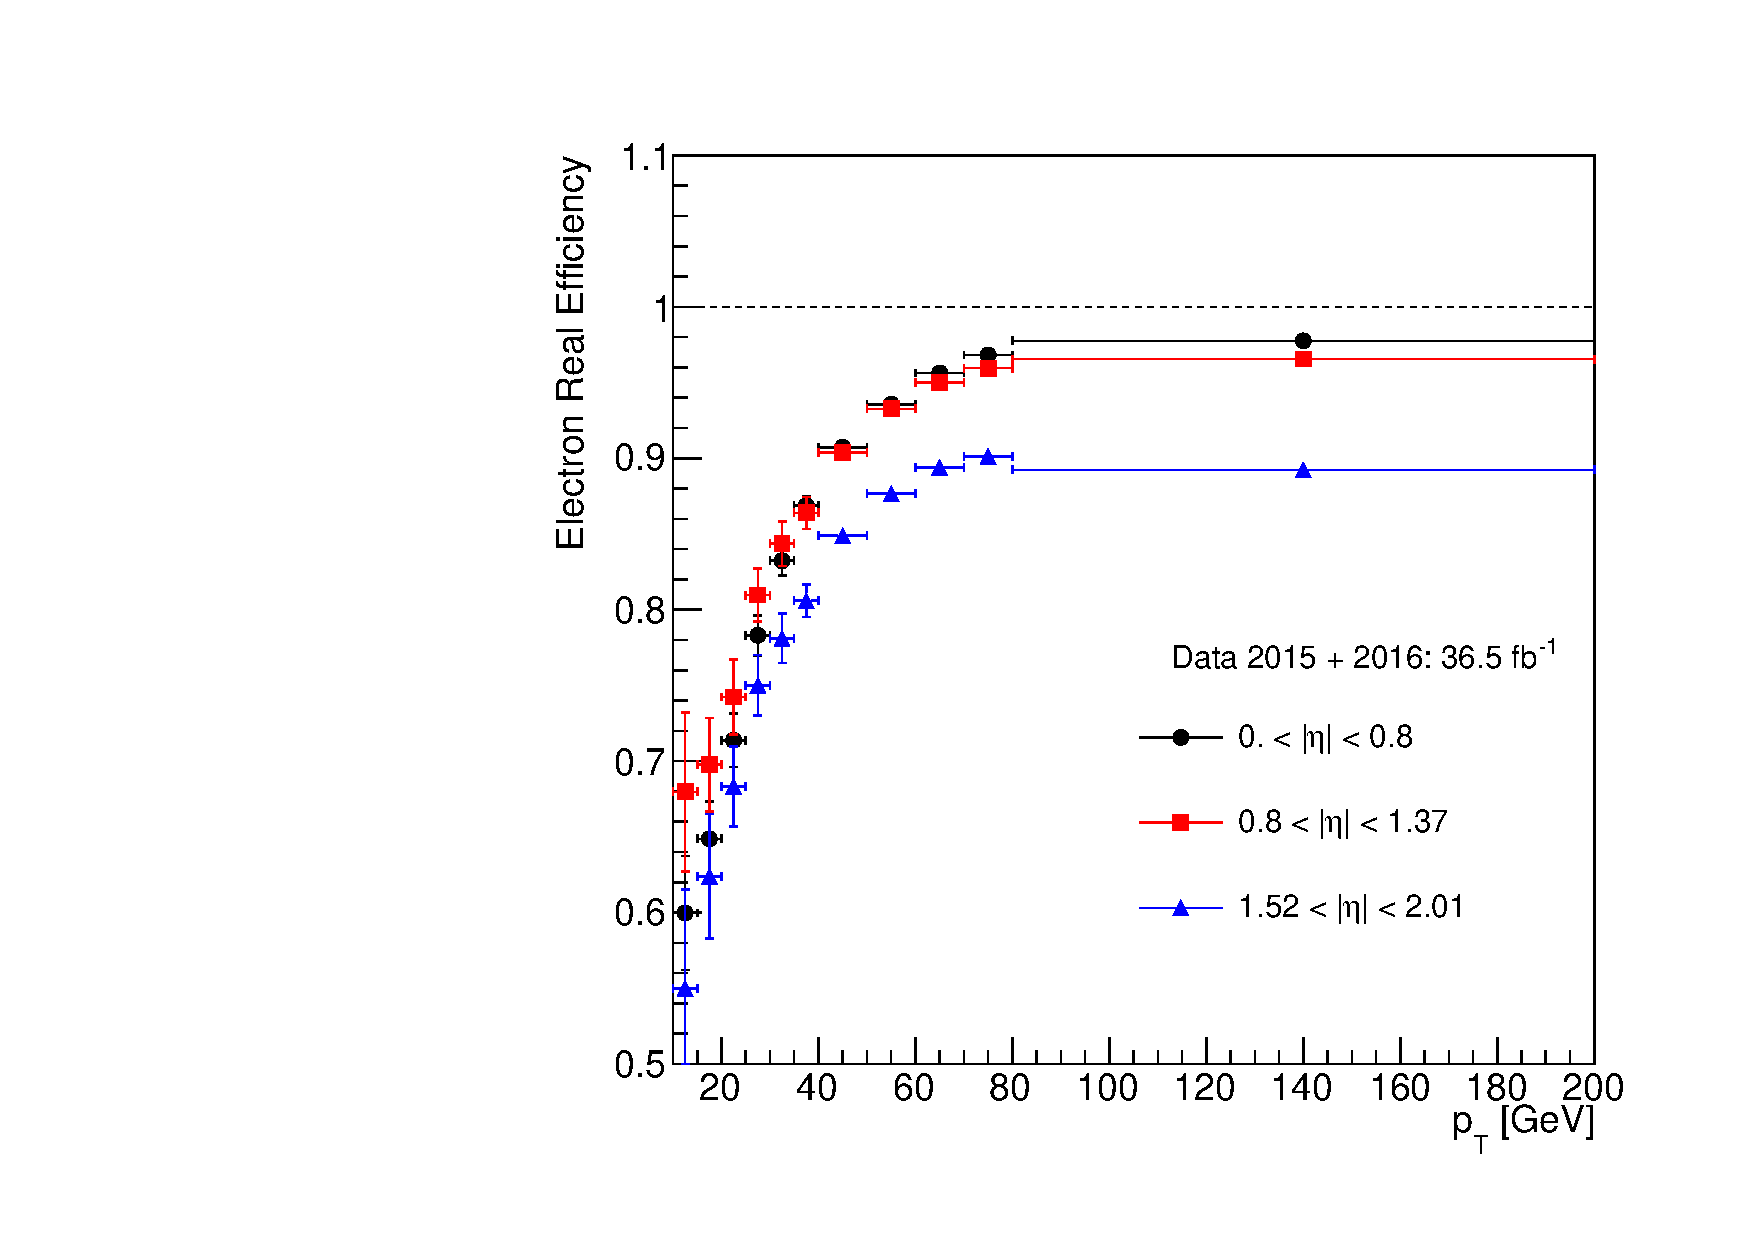
\includegraphics[width=\textwidth]{real_electron_efficiency_total_systematics.pdf}
\subcaption{Electrons}
\end{subfigure}
\begin{subfigure}{0.49\textwidth}
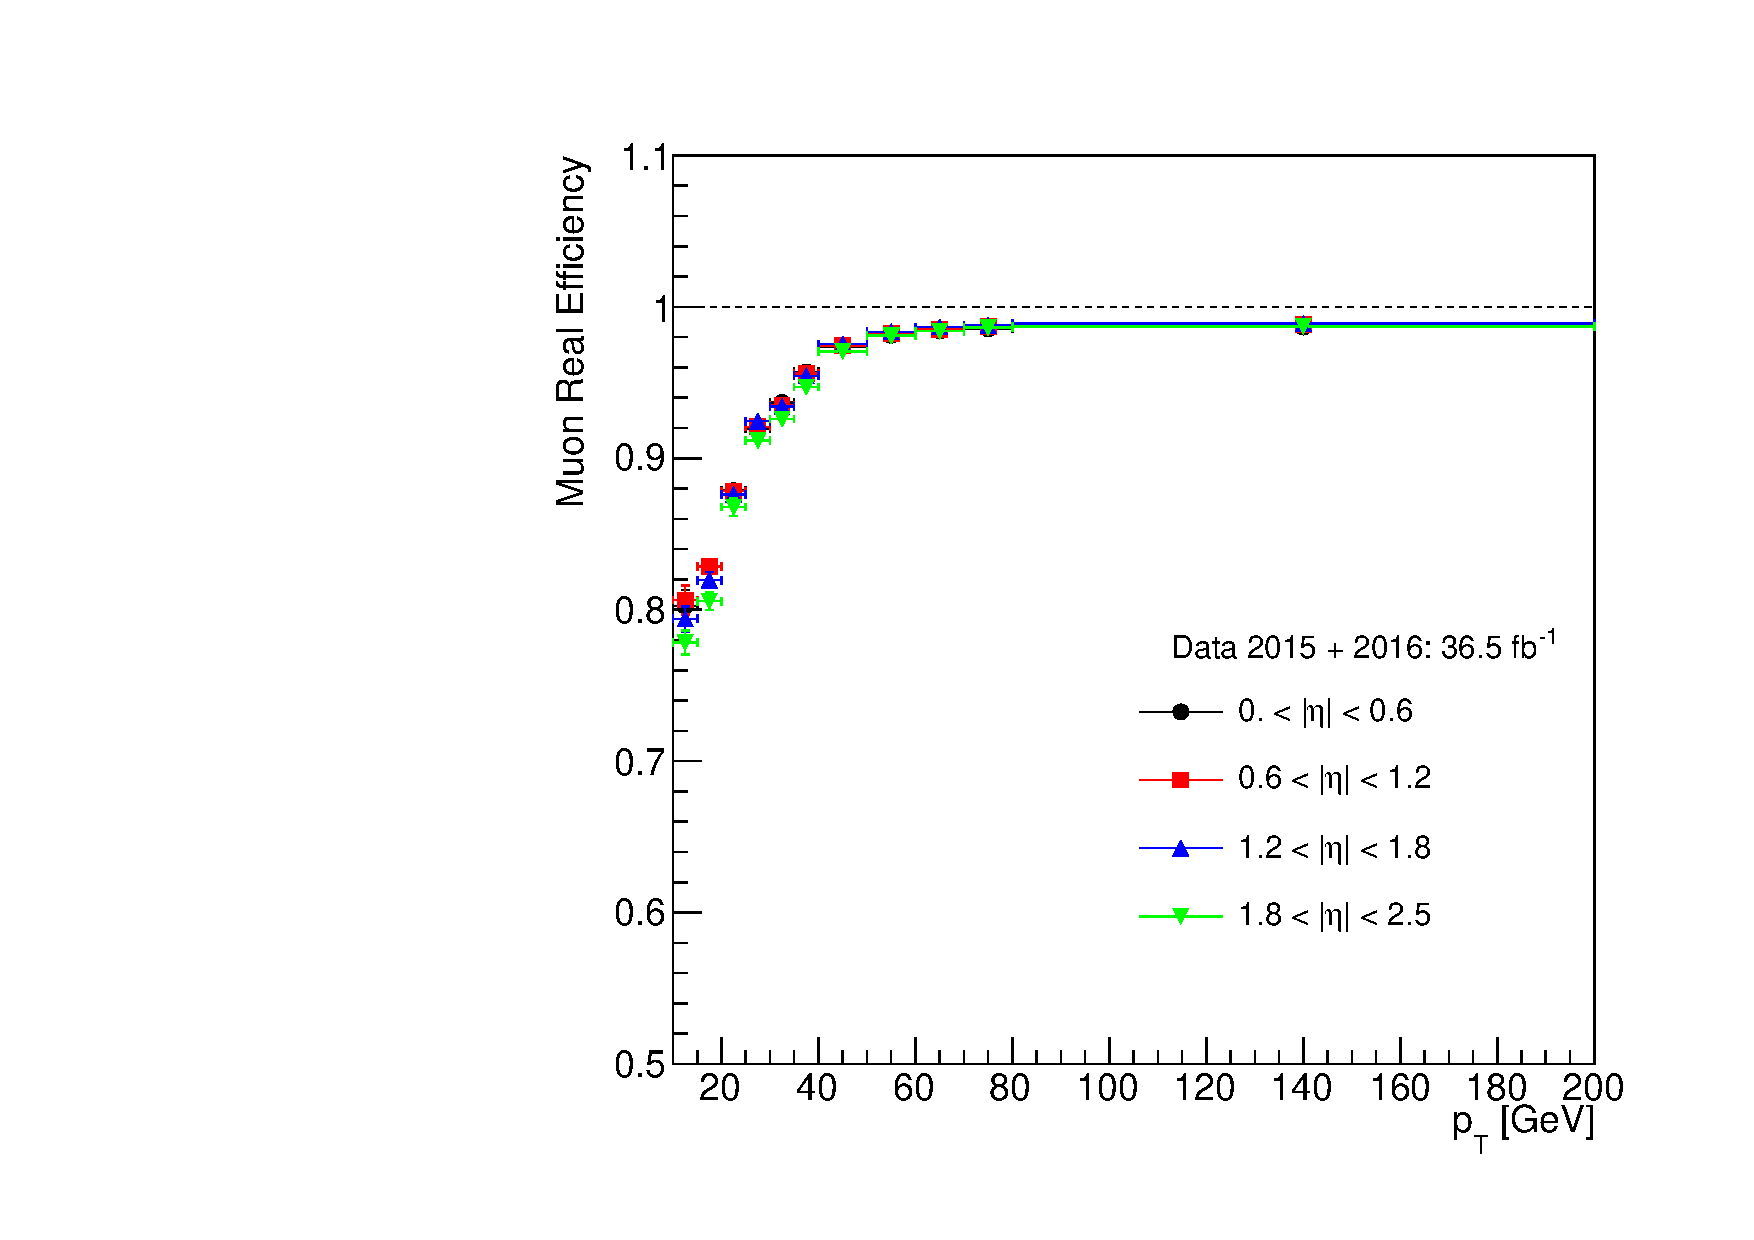
\includegraphics[width=\textwidth]{real_muon_efficiency_total_systematics.pdf}
\subcaption{Muons}
\end{subfigure}
\caption{Baseline-to-signal efficiencies as a function of $\pt$ and $|\eta|$ for real electrons (left) and muons (right), measured in 2015+2016 data.
%The background subtraction is applied on the electron channel only.
The $|\eta|$ binning used in the electron case corresponds to the geometry of the electromagnetic calorimeter.
For muons a homogeneous $|\eta|$ binning is considered.
The error bars corresponds to the quadratic sum of the statistical and tag-and-probe measurement systematic uncertainties.}
\label{fig:prompt_leptons_eff}
\end{figure}

The efficiency is measured as a function of \pt\ and $\eta$, and the results are presented in Fig~\ref{fig:prompt_leptons_eff} for electrons and muons. 
The background subtraction is applied on the electron channel only. 
The following systematic uncertainties are assigned to the measured efficiencies: 

\begin{itemize}
\item[$\bullet$] Background contamination: 27 variations of the tag-and-probe method are considered to assess the electron measurement systematics.
Three $m_{ee}$ windows and 9 variations of the background subtraction methods are considered.
The largest contribution to the systematics arises from the $m_{ee}$ window variation.
This is expected as the proportion of electrons affected by bremsstrahlung depends on $m_{ee}$.
The resulting relative systematics vary from 6\% $\sim$ 12\% in the $10<\pt<15 \GeV$ region, 3\% to 6\% in the $15<\pt<20 \GeV$ region, 1\% to 3\% in the $20<\pt<40 \GeV$ region, and less than 1\% for $\pt >$ 40 GeV.
The systematic uncertainties associated to the muon efficiencies measurement vary from 1\% to 1.3\% in the $10<\pt<15 \GeV$ region and less then 1\%for $\pt >$ 15 GeV. 
\item[$\bullet$] Trigger: a systematic uncertainty accounting for a potential bias at trigger level is considered as last year.% It varies between 0 and 4\%, depending on the \pt range.
\item[$\bullet$] Extrapolation to busy environments: efficiencies are typically lower in such environments due to the proximity of jets and leptons; 
an uncertainty is assigned by comparing efficiencies in simulated $Z\to\ell\ell$ and $\gluino\to\ttbar\neut$ events, for $\Delta m(\gluino,\neut)>1 \TeV$ which represents an extreme case of final states with highly boosted top quarks. 
The uncertainty, taken as the difference in efficiencies, is parametrized as a function of \pt\ and $\Delta R$ (the angular distance between the lepton and the closest jet). 
\end{itemize}
%The resulting systematic uncertainties are summarized in Table~\ref{tab:RLE_systematics_bkg} and Table~\ref{tab:RLE_systematics_busy}. 
The resulting systematic uncertainties are summarized in Table~\ref{tab:RLE_systematics_all} and Table~\ref{tab:RLE_systematics_busy}.


\begin{center}
\begin{table}
\resizebox{\textwidth}{!}{%
\begin{tabular}{cccc|cccc}
\hline
\hline
& \multicolumn{3}{c}{Electrons} & \multicolumn{3}{c}{Muons}\\
& $0<|\eta|<0.8$ & $0.8<|\eta|<1.37$ & $1.52<|\eta|<2.01$ & $0<|\eta|<0.6$ & $0.6<|\eta|<1.2$ & $1.2<|\eta|<1.8$ & $1.8<|\eta|<2.5$\\
\hline
10 GeV $< p_{\text T} <$ 15 GeV & 0.047 & 0.063 & 0.089 & 0.014 & 0.010 & 0.008 & 0.011\\
15 GeV $< p_{\text T} <$ 20 GeV & 0.027 & 0.042 & 0.062 & 0.005 & 0.006 & 0.008 & 0.011\\
20 GeV $< p_{\text T} <$ 25 GeV & 0.018 & 0.031 & 0.041 & 0.003 & 0.006 & 0.010 & 0.010\\
25 GeV $< p_{\text T} <$ 30 GeV & 0.029 & 0.024 & 0.027 & 0.011 & 0.015 & 0.022 & 0.019\\
30 GeV $< p_{\text T} <$ 35 GeV & 0.023 & 0.021 & 0.023 & 0.007 & 0.009 & 0.014 & 0.011\\
35 GeV $< p_{\text T} <$ 40 GeV & 0.014 & 0.018 & 0.018 & 0.004 & 0.004 & 0.006 & 0.006\\
40 GeV $< p_{\text T} <$ 50 GeV & 0.007 & 0.010 & 0.010 & 0.002 & 0.001 & 0.002 & 0.001\\
50 GeV $< p_{\text T} <$ 60 GeV & 0.008 & 0.010 & 0.010 & 0.001 & 0.001 & 0.001 & 0.001\\
60 GeV $< p_{\text T} <$ 70 GeV & 0.007 & 0.010 & 0.010 & 0.001 & 0.001 & 0.001 & 0.002\\
70 GeV $< p_{\text T} <$ 80 GeV & 0.008 & 0.011 & 0.012 & 0.002 & 0.001 & 0.001 & 0.002\\
80 GeV $< p_{\text T} <$ 120 GeV & 0.010 & 0.010 & 0.011 & 0.004 & 0.002 & 0.002 & 0.002\\
120 GeV $< p_{\text T} <$ 150 GeV & 0.005 & 0.005 & 0.011 & 0.006 & 0.005 & 0.005 & 0.005\\
150 GeV $< p_{\text T} <$ 200 GeV & 0.005 & 0.002 & 0.019 & 0.005 & 0.005 & 0.005 & 0.006\\
\hline
\hline
\end{tabular}
}
\caption{
Systematic uncertainties on the measured real lepton efficiency, separating sources affecting the measurement itself (background subtraction, trigger bias, and different methods). See appendix~\ref{subsec:RLE_sources_of_systematic_uncertainties} for more details about the sources of the systematic uncertainties.
}
\label{tab:RLE_systematics_all}
\end{table}
\end{center}

\begin{center}
\begin{table}
\resizebox{\textwidth}{!}{%
\begin{tabular}{ccccccccccc}
\hline
\hline
\multicolumn{9}{c}{electrons (busy environments)}\\
\hline
$\Delta R(e, jet)$ & [0, 0.1] & [0.1, 0.15] & [0.15, 0.2] & [0.2, 0.3] & [0.3, 0.35] & [0.35, 0.4] & [0.4, 0.6] & [0.6, 4]\\
\hline
10 GeV $< p_{\text T} <$ 20 GeV & - & - & - & - & - & - & 25.31\% & 6.5\%\\
20 GeV $< p_{\text T} <$ 30 GeV & - & - & - & - & - & 73.37\% & 10.21\% & 0.37\%\\
30 GeV $< p_{\text T} <$ 40 GeV & - & - & - & 97.71\% & 48.22\% & 15.54\% & 7.29\% & 0.58\%\\
40 GeV $< p_{\text T} <$ 50 GeV & - & - & - & 52.81\% & 22.80\% & 16.73\% & 7.68\% & 1.10\%\\
50 GeV $< p_{\text T} <$ 60 GeV & - & - & - & 29.96\% & 21.49\% & 20.23\% & 6.99\% & 2.78\%\\
60 GeV $< p_{\text T} <$ 80 GeV & - & - & 55.89\% & 24.31\% & 17.40\% & 24.77\% & 6.20\% & 2.87\%\\
80 GeV $< p_{\text T} <$ 150 GeV & - & 57.52\% & 30.24\% & 16.45\% & 12.73\% & 20.92\% & 4.44\% & 2.73\%\\
150 GeV $< p_{\text T} <$ 200 GeV & 88.54\% & 40.16\% & 19.34\% & 8.45\% & 14.66\% & 16.57\% & 2.57\% & 1.90\%\\
\hline
\hline
%\end{tabular}
%}
%\resizebox{\textwidth}{!}{%
%\begin{tabular}{ccccccccccc}
%\hline
%\hline
\multicolumn{9}{c}{muons (busy environments)}\\
\hline
$\Delta R(\mu, jet)$ & [0, 0.1] & [0.1, 0.15] & [0.15, 0.2] & [0.2, 0.3] & [0.3, 0.35] & [0.35, 0.4] & [0.4, 0.6] & [0.6, 4]\\
\hline
10 GeV $< p_{\text T} <$ 20 GeV & - & - & - & - & - & - & 33.59\% & 5.18\%\\
20 GeV $< p_{\text T} <$ 30 GeV & - & - & - & - & - & 82.34\% & 22.27\% & 3.39\%\\
30 GeV $< p_{\text T} <$ 40 GeV & - & - & -  & 98.54\% & 56.36\% & 31.89\% & 14.22\% & 2.24\%\\
40 GeV $< p_{\text T} <$ 50 GeV & - & - & - & 53.10\% & 21.33\% & 13.90\% & 6.81\% & 1.45\%\\
50 GeV $< p_{\text T} <$ 60 GeV & - & - & - & 24.98\% & 13.72\% & 9.62\% & 3.83\% & 0.79\%\\
60 GeV $< p_{\text T} <$ 80 GeV & - & - & 44.41\% & 13.75\% & 6.14\% & 4.76\% & 2.04\% & 0.15\%\\
80 GeV $< p_{\text T} <$ 150 GeV & - & 29.94\% & 7.14\% & 3.16\% & 1.30\% & 1.04\% & 0.07\% & 0.57\%\\
150 GeV $< p_{\text T} <$ 200 GeV & 82.26\% & 4.14\% & 1.02\% & 0.17\% & 0.29\% & 0.62\% & 1.02\% & 1.13\%\\
\hline
\hline
\end{tabular}
}
\caption{
Systematic uncertainties on the measured real lepton efficiency, due to the extrapolation to busy environments using $\gluino \to \ttbar \tilde{\chi_1^0}$ events. See appendix~\ref{subsec:RLE_sources_of_systematic_uncertainties} for more details.
}
\label{tab:RLE_systematics_busy}
\end{table}
\end{center}


\subsection{MC Template Method}
We describe in this section a simulation-based method that provides an alternative estimate of the data-driven backgrounds described in Sections ~\ref{sec:chargeflip} and ~\ref{subsec:fakes_matrix}. 
 %More details about the method can be found in Appendix \ref{app_mc_template}.

The MC-based method relies on kinematic distributions from MC simulations to extrapolate background predictions from 
control regions with low \met , \meff , 
and jet multiplicity to the signal regions (where \met , \meff , or jet multiplicity are required to be high). 
The control regions are used to reweight MC simulation of \ttbar\ and $V+$ jets events to match the observed data 
by extracting correction factors which depend on the identified origin of the fake or non-prompt lepton. 
The main assumption of the method is that the MC simulations describe the kinematic distributions correctly 
and predict accurately the rate of fake leptons up to a global factor (for each type of fake lepton) 
independent of the event kinematics and the process type. This assumption makes the method a suitable cross-check of the matrix method, 
that assumes that the lepton fake rates are the same in control and signal regions regardless of the selection requirements. 
The other assumption the MC template method makes is that the fake rates are uncorrelated in events with multiple fake leptons 
which is expected to be negligeable.

Six non-overlapping control regions are defined by the presence of $b$-jets and by the flavors of the same sign lepton pair in the event:
\begin{itemize}
\item CR0b: events without $b$-jets in $ee$, $e\mu$, and $\mu\mu$ channels.
\item CR1b: events with at least one $b$-jet in $ee$, $e\mu$, and $\mu\mu$ channels.
\end{itemize}
All the selected events contain two or more same-sign signal leptons and \met >40 GeV and 2 or more jets. 
Events satisfying the signal regions requirements are excluded from the control regions. 
The purpose of the \met requirement is to remove multi-jet events that have two or more ``fake'' leptons and tend to have low \met. 

The next step is to classify events into separate categories depending on the lepton origin. 
The three main categories are prompt isolated leptons, charge flipped electrons, 
and ``fake'' leptons which consist of non-prompt leptons coming from hadron decays and hadrons misidentified as leptons. 
The fakes are further separated by the lepton flavor ($e$ or $\mu$) and by the jet flavor producing the fake lepton. 
We separate the leptons that are coming from $b$-hadron decays, 
labelled as heavy-flavor (HF), from the rest of the fakes, labelled as light-flavor (LF), and derive a fake rate correction for 
each category. The purpose of this separation is to make the $b$-tagging requirement orthogonal to the fake rate correction. 
The classification is done based on the parent particle from the generator event record using the type and origin of the lepton provided 
by the MCTruthClassifier.

In total we have five categories (charge flip, EL HF, MU HF, EL LF, MU LF) that we derive correction factors for using a simulatenous fit to data in six control regions (CR0b and CR1b for $ee$, $e\mu$, and $\mu\mu$ channels).
The fit uses a likelihood function defined as the product of the Poisson probabilities describing the observed events in the binned 
distributions from the expected number 
of events rescaled by the five correction factors which are left free to float in the fit.  
These correction factors are applied to the MC predictions in the signal regions to obtain an estimation of the fake and charge flip backgrounds. 

The six distributions are chosen for variables that provide the best separation between processes with prompt leptons and processes with fake leptons and charge flip and are shown 
before and after the fit in Figures \ref{f:prefit_CR0b}-\ref{f:prefit_CR1b} and Figures \ref{f:postfit_CR0b}-\ref{f:postfit_CR1b}, respectively. 

 \begin{figure}[htb]
   \includegraphics[width=.32\textwidth]{Prefit/el2_pt_ee_CR0b_SS3L}
   \includegraphics[width=.32\textwidth]{Prefit/NJETS_em_CR0b_SS3L}
   \includegraphics[width=.32\textwidth]{Prefit/mu2_pt_mm_CR0b_SS3L}
 \caption{
 Pre-fit distributions for  $ee$ channel (left),  for  $e\mu$ channel (middle), and  for  $\mu\mu$ channel (right) from CR0b that were used in the fit to extract the fake rate and charge flip corrections.
The generator used in these plots is Powheg. The hashed band represents the sum of systematic uncertainties on the predictions.
 \label{f:prefit_CR0b}
 }
 \end{figure}

\begin{figure}[htb]
  \includegraphics[width=.32\textwidth]{Postfit/el2_pt_ee_CR0b_SS3L}
  \includegraphics[width=.32\textwidth]{Postfit/NJETS_em_CR0b_SS3L}
  \includegraphics[width=.32\textwidth]{Postfit/mu2_pt_mm_CR0b_SS3L}
\caption{
Post-fit distributions for  $ee$ channel (left),  for  $e\mu$ channel (middle), and  for  $\mu\mu$ channel (right) from CR0b that were used in the fit to extract the fake rate and charge flip corrections.
The generator used in these plots is Powheg. The hashed band represents the sum of systematic uncertainties on the predictions.
\label{f:postfit_CR0b}
}
\end{figure}

 \begin{figure}[htb]
   \includegraphics[width=.32\textwidth]{Prefit/el2_pt_ee_CR1b_SS3L}
   \includegraphics[width=.32\textwidth]{Prefit/NJETS_em_CR1b_SS3L}
   \includegraphics[width=.32\textwidth]{Prefit/mu2_pt_mm_CR1b_SS3L}
 \caption{
 Pre-fit distributions for  $ee$ channel (left), for  $e\mu$ channel (middle), and  for  $\mu\mu$ channel (right) from CR1b that were used in the fit to extract the fake rate and charge flip corrections.
The generator used in these plots is Powheg. The hashed band represents the sum of systematic uncertainties on the predictions.
 \label{f:prefit_CR1b}
 }
 \end{figure}

\begin{figure}[htb]
  \includegraphics[width=.32\textwidth]{Postfit/el2_pt_ee_CR1b_SS3L}
  \includegraphics[width=.32\textwidth]{Postfit/NJETS_em_CR1b_SS3L}
  \includegraphics[width=.32\textwidth]{Postfit/mu2_pt_mm_CR1b_SS3L}
\caption{
Post-fit distributions for  $ee$ channel (left), for  $e\mu$ channel (middle), and  for  $\mu\mu$ channel (right) from CR1b that were used in the fit to extract the fake rate and charge flip corrections.
The generator used in these plots is Powheg. The hashed band represents the sum of systematic uncertainties on the predictions.
\label{f:postfit_CR1b}
}
\end{figure}

The minimization of the negative log likelihood using the \textsc{Minuit} package leads 
to the correction factor shown in Tables \ref{t:fake_factors_powheg} and \ref{t:fake_factors_sherpa}.
The tables represent the correction factors obtained from the fit upon using two different parton showers, Pythia and Sherpa
for the processes that lead to non-prompt leptons and charge flips.
The goal of varying the parton shower is to access the dependence of the fake and charge flip estimates on the choice of the 
parton shower. An additional systematic uncertainty is added to account for this dependency. 
The uncertainties in the correction factors themselves correspond to how much the parameter needs to be varied for 
a one standard deviation change in the likelihood function. This uncertainty takes into account the limited number of simulated events and is included as a 
systematic uncertainty on the expected number of background events. 


\begin{table}[htb]
  \caption{The fake-rate and charge flip corrections obtained after minimizing the likelihood function using Pythia.
    The uncertainty in the corrections takes into account the limited statistics of simulated events.
    \label{t:fake_factors_powheg}}
  \centering
  % % \scalebox{0.85}{
   \begin{tabular}{|c|c|c|}
          \hline
          Category & Correction & Uncertainty  \\
          \hline
          chFlip & 1.49 & 0.58 \\ 
          HF EL & 2.80 & 0.98 \\
          LF EL & 2.89 & 0.88 \\
          HF MU & 1.59 & 0.31 \\
          LF MU & 1.00 & 1.34 \\
          \hline
        \end{tabular}
  % % }                                                                            
\end{table}

\begin{table}[htb]
  \caption{The fake-rate and charge flip corrections obtained after minimizing the likelihood function using Sherpa.
    The uncertainty in the corrections takes into account the limited statistics of simulated events.
    \label{t:fake_factors_sherpa}}
  \centering
  % % \scalebox{0.85}{
  \begin{tabular}{|c|c|c|}
    \hline
    Category & Correction & Uncertainty  \\
    \hline
    chFlip & 1.34 & 0.58 \\ 
    HF EL & 2.40 & 0.85 \\
    LF EL & 1.83 & 1.04 \\
    HF MU & 1.17 & 0.16 \\
    LF MU & 2.40 & 0.81 \\
    \hline
  \end{tabular}                                                                                         
  % % }                                                                            
\end{table}


The MC template method is validated by looking at the Data/MC agreement near the signal regions where we invert one of the cuts while keeping the last bin corresponding to the SR blinded. These distributions can be found in Appendix~\ref{app:mctemplate}.

After applying the correction factors of Table \ref{t:fake_factors_powheg} to obtain the nominal fake estimates with the samples shown 
in Table \ref{t:samples_pythia}, 
an additional uncertainty on the rate of fake leptons from \ttbar and $V$+jets in the signal region is assigned by repeating the background evaluation 
procedure using samples with Sherpa shown in Tables~\ref{t:samples_sherpa1}-\ref{t:samples_sherpa2} and with the correction factors from 
Table \ref{t:fake_factors_sherpa}. 
In practice, only \ttbar contributes to the SRs and the final yields with systamtic uncertainties from 
fit uncertainty, theory uncertainties on ttbar, comparison of different showers (Pythia 6 and Sherpa) is shown in Table \ref{tab:fakes_mcglobal}.
This table also shows a global correction factor derived by taking the ratio of the weighted \ttbar to raw MC \ttbar with
a global uncertainty that includes all systematic uncertainties used to obtain the final estimate. 


\begin{table}[!htb]
\caption{Expected yields for background processes with fake leptons,
in the signal regions with a global correction factor that represents the ratio of weighted \ttbar to raw MC \ttbar with
a global uncertainty that includes: fit uncertainty, theory uncertainties on ttbar, comparison of different showers. 
The fraction of the systematic uncertainty from the comparison between two showers (Pythia and Sherpa) is also shown.
}
\label{tab:fakes_mcglobal}
\centering
\resizebox{\textwidth}{!}{
\begin{tabular}{|c||c|c|c||}\hline
Region &              MC Template method  & Global correction & Shower systematic \\
\hline
Rpc2L0bH & $1.00 \pm 0.96 \pm 0.81$ & $2.80 \pm 2.10$ & 74\% \\
Rpc2L0bS & $1.68 \pm 1.02 \pm 1.26$ & $2.89 \pm 1.97$ & 65\% \\
Rpc2L1bH & $2.07 \pm 0.63 \pm 1.56$ & $1.22 \pm 1.14$ & 34\% \\
Rpc2L1bS & $2.33 \pm 1.17 \pm 2.10$ & $1.83 \pm 1.42$ & 81\% \\
Rpc2L2bH & $<0.5$ & $0 \pm 0$ & 0\% \\
Rpc2L2bS & $0.41 \pm 0.33 \pm 0.45$ & $1.47 \pm 1.12$ & 73\% \\
Rpc2Lsoft1b & $2.48 \pm 1.32 \pm 1.86$ & $1.59 \pm 1.31$ & 68\% \\
Rpc2Lsoft2b & $1.66 \pm 0.66 \pm 1.28$ & $1.72 \pm 1.29$ & 54\% \\
Rpc3L0bH & $<0.5$ & $0 \pm 0$ & 0\% \\
Rpc3L0bS & $0.21 \pm 0.15 \pm 0.16$ & $2.90 \pm 2.20$ & 71\% \\
Rpc3L1bH & $0.42 \pm 0.29 \pm 0.32$ & $1.59 \pm 1.25$ & 59\% \\
Rpc3L1bS & $3.55 \pm 1.80 \pm 2.76$ & $1.76 \pm 1.32$ & 67\% \\
Rpc3LSS1b & $0.90 \pm 0.14 \pm 0.69$ & $2.34 \pm 1.44$ & 56\% \\
Rpv2L0b & $1.02 \pm 0.96 \pm 0.76$  & $2.80 \pm 2.10$ & 66\% \\
Rpv2L1bH & $0.60 \pm 0.35 \pm 0.48$ & $1.32 \pm 0.92$ & 45\% \\
Rpv2L1bM & $1.20 \pm 0.69 \pm 0.95$ & $1.59 \pm 1.25$ & 58\% \\
Rpv2L1bS & $4.46 \pm 1.67 \pm 3.45$ & $1.33 \pm 0.80$ & 67\% \\
Rpv2L2bH & $<0.5$ & $0 \pm 0$ & 0\% \\
Rpv2L2bS & $7.24 \pm 2.36 \pm 5.43$ & $2.45 \pm 1.83$ & 73\% \\
\hline
\hline
\end{tabular}
}
\end{table}



\subsection{Background processes with charge-flipped electrons}
The lepton charge mis-measurement commonly referred to as ``charge flip'', 
is an experimental background strongly associated to analyses relying on same-sign leptons final states. 
In those events, the electric charge of one of the two leptons forming an opposite-sign (OS) pair, 
coming from an abundant SM process ($pp\to Z$, \ttbar, $W^+W^-$\ldots), 
is mis-identified leading to a much rarer SS pair event.
In most cases, the source of such a misidentification 
is the creation of additional close-by tracks $e^\pm\to e^\pm\gamma\to e^\pm e^\pm e^\mp$ 
via bremmstrahlung of the original electron when interacting with the material of the inner tracker. 
If one of the secondary electron tracks is subsequently preferred to the original track in the reconstruction of the electron candidate, 
the charge assigned to the electron might be incorrect, leading to a charge-flip event. 
Errors on the track charge assignment itself may occur as well, but they are much rarer. 
In the case of muons, charge-flip is essentially negligible due to the much smaller interaction cross-section with matter, 
and the requirement of identical charges to be measured for the inner tracker and muon spectrometer tracks. 

We rely on a purely data-driven method (same in the previous version of the analysis~\cite{ATLAS-CONF-2016-037}) to estimate event yields for the electron charge-flip background. 
Assuming one knows the electron charge flip rates $\xi(\eta,\pt)$, 
a simple way to predict these yields is to select events with pairs of opposite-sign leptons in data and assign them a weight:

\begin{align}
w_\text{flip} = \xi_1(1-\xi_2) + (1-\xi_1)\xi_2
\label{eqn:chargeflip_weight}
\end{align}
where $\xi_{(i)}=0$ for muons.

The advantages of this method are a good statistical precision since the charge flip rate is quite small, 
and the absence of dependency to the simulation and related uncertainties. 
Obviously, it requires a precise measurement of the rates, which is described in this section. 
An inconvenience of this approach is that the reconstructed momentum for charge-flipped electrons  
tends to be negatively biased (too low by a few GeV), 
since such important bremmstrahlung topologies represent only 
a very small fraction of the cases used to tune electron energy calibration. 
Simply re-weighting electrons from opposite-sign lepton pairs therefore does not predict correctly 
the charge-flip background shape for variables very sensitive to the electron momentum, for example the $m_{ee}$ lineshape. 
Further, we neglect this bias. 

For the nominal (tight) estimate of the charge-flip background contributions, only events with exactly two OS signal electrons are considered. 
Corrections in the fake lepton estimate however require estimating as well charge-flip contributions for selections involving 
baseline electrons failing signal requirements (see section~\ref{subsubsec:fakes_matrix_descr}); 
for that reason, the charge-flip (loose) rate is measured for these two categories of electrons. 

\subsection{Methodology}
\label{subsec:chargeflip_method}

\begin{figure}[t!]
\centering
\begin{subfigure}[b]{0.45\textwidth}
	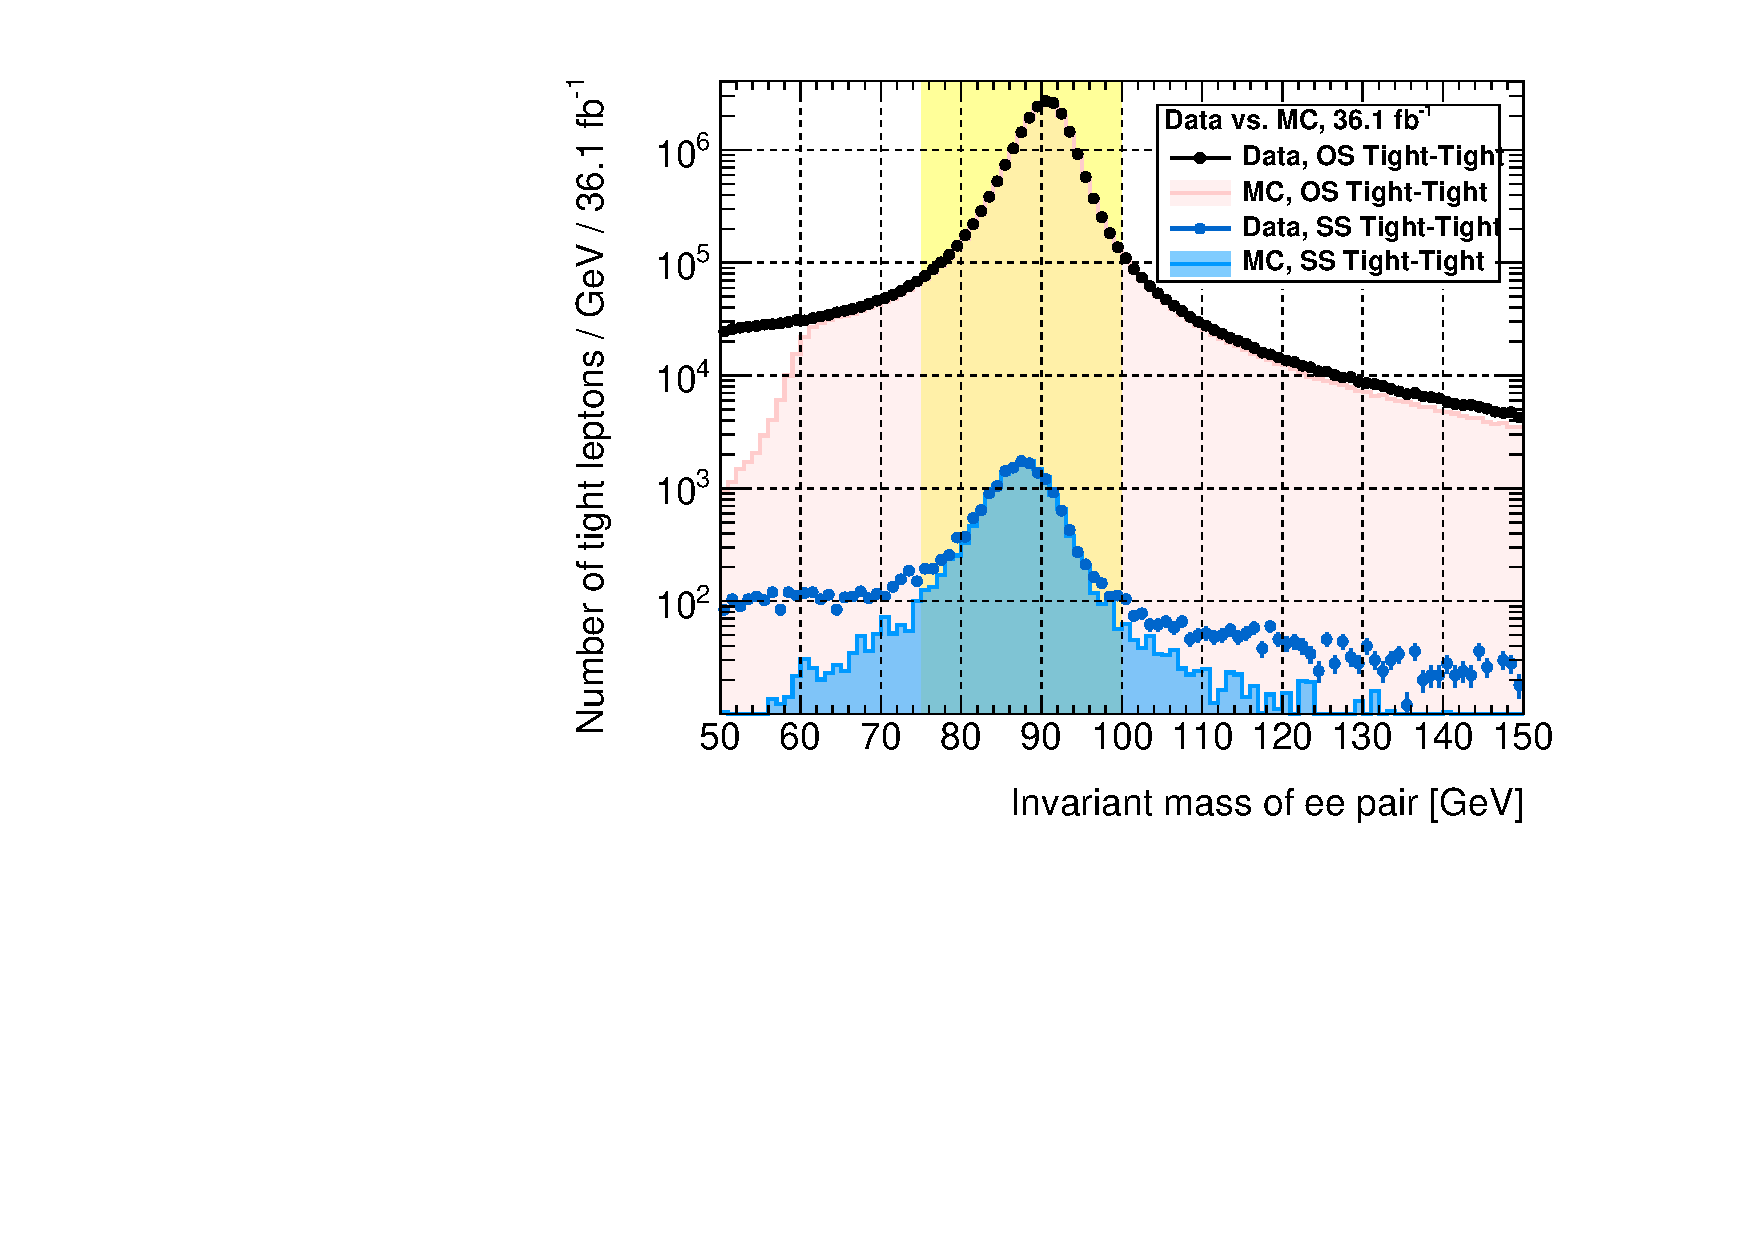
\includegraphics[width=\textwidth]{Data_vs_MC_Pass_EL}
\end{subfigure}
\begin{subfigure}[b]{0.45\textwidth}
	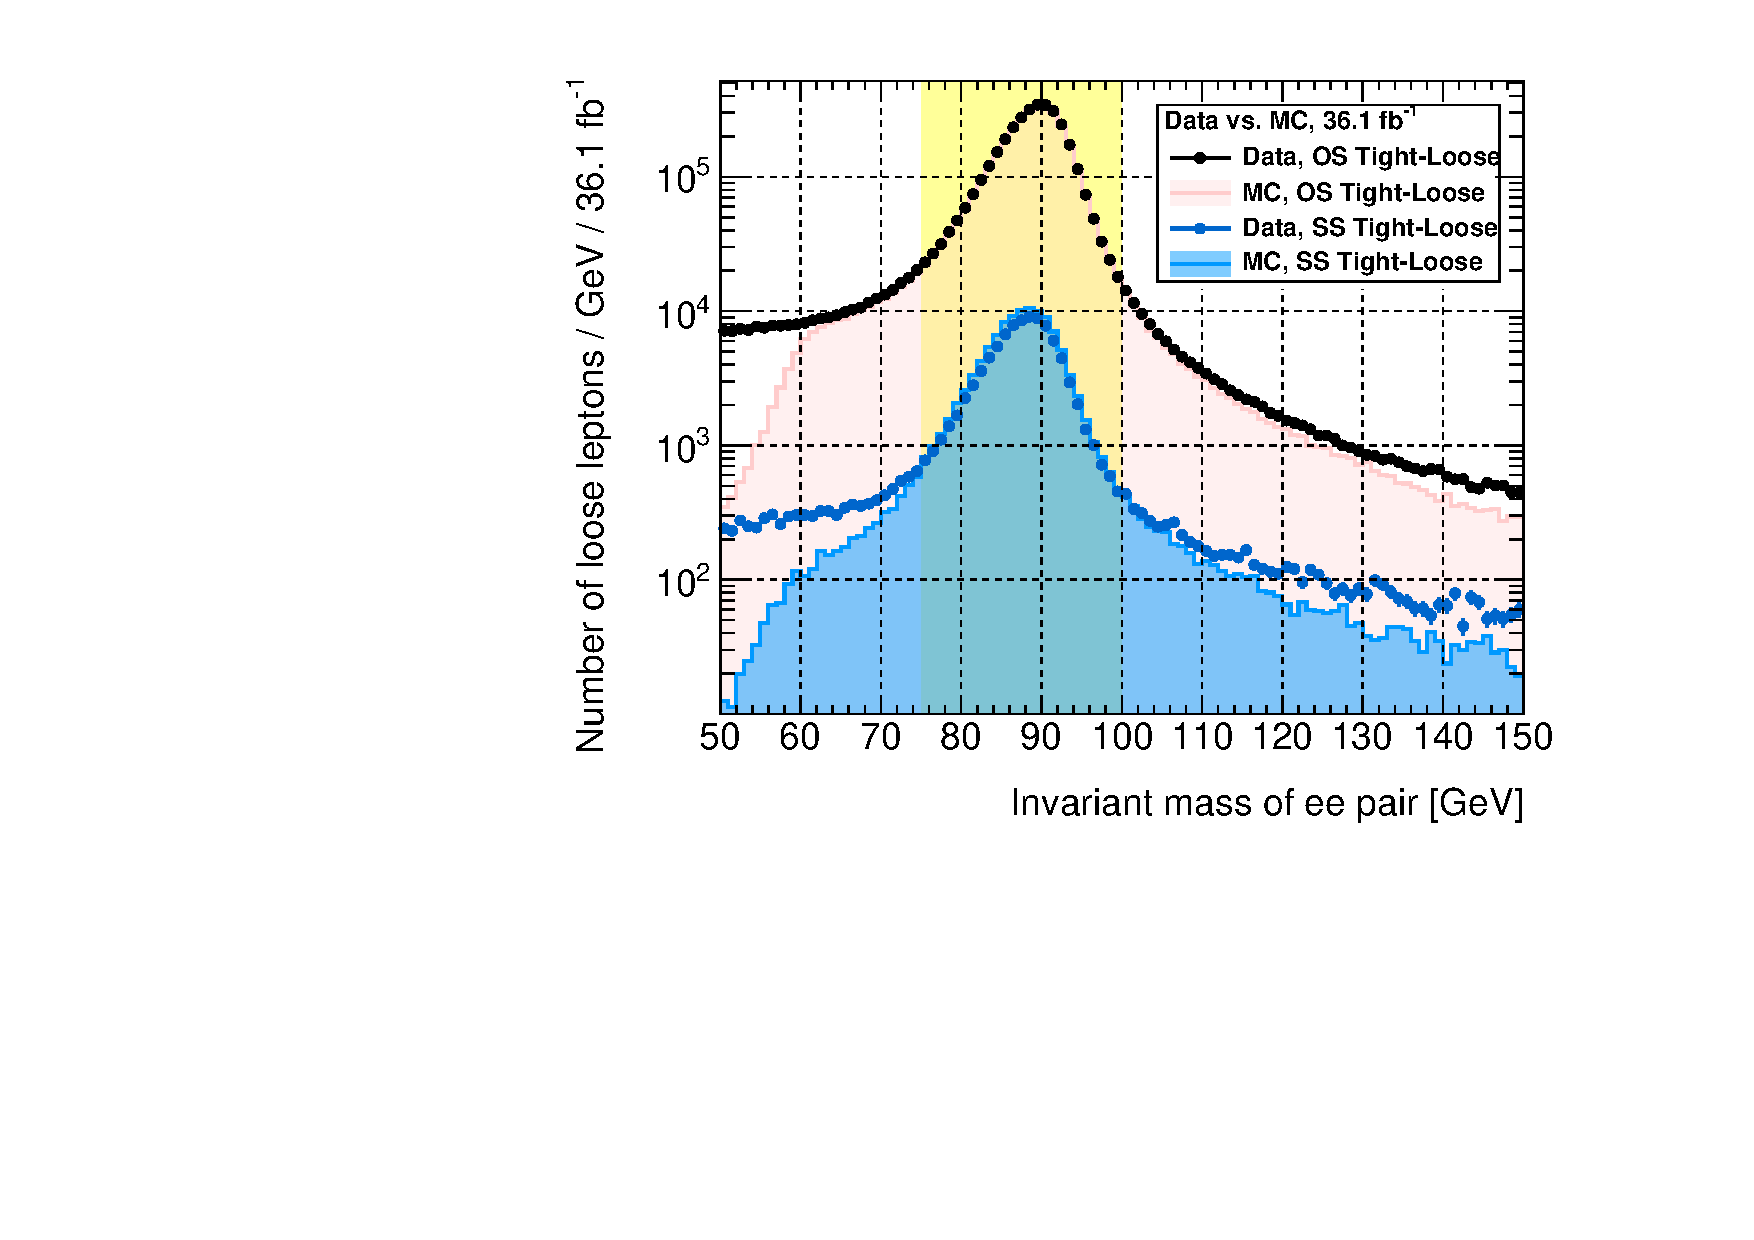
\includegraphics[width=\textwidth]{Data_vs_MC_Fail_EL}
\end{subfigure}
\caption{Invariant mass of opposite- and same-sign electron pairs, 
when both electrons satisfy signal requirements (left) or one of them fails them (right). Drell-Yan MC samples are not included, thus the drop in the MC distributions (light magenta filled area).}
\label{fig:chargeflip_mee}
\end{figure}

Charge-flip rates are measured in data relying on a clean $Z\to ee$ sample ($75<m_{ee}<100 \GeV$), 
in which the rates can be determined from the relative proportions of OS and SS electron pairs. 
Figure~\ref{fig:chargeflip_mee} illustrates this event selection. 
The rates are measured as function of $\eta$ and \pt, to follow their dependency to the distribution of material in the detector, 
the bremmstrahlung emission rate, and the track curvature. 
Because of this binned measurements, and that the two electrons in a given pair generally have different kinematic properties, 
it has been found that the most efficient and less biased use of the available statistics 
is obtained by simultaneously extracting the rates in all bins via the maximization of the likelihood function describing the 
Poisson-expected yields of SS pairs: 

\begin{align}
L(\{N^\text{SS,obs}_\varpi\}|\{\xi(\eta,\pt)\}) 
= \prod_{\varpi} \mathcal P\left(N^\text{SS,obs}_\varpi|w_\text{flip}(\xi(\eta_1,p_{\mathrm{T},1}),\xi(\eta_2,p_{\mathrm{T},2}))\times N^\text{OS+SS,obs}_\varpi\right)
\label{eqn:chargeflip_likelihood}
\end{align}
with $\varpi=(\eta_1,p_{\mathrm{T},1},\eta_2,p_{\mathrm{T},2})$ indexing bins, where (arbitrarily) $p_{\mathrm{T},1}>p_{\mathrm{T},2}$; 
the expression of $w_\text{flip}$ is given by~(\ref{eqn:chargeflip_weight}). 
Statistical uncertainties on the extracted charge-flip rates are obtained (in a standard way) from the likelihood's numerically-computed Hessian matrix. 

In the nominal charge-flip measurement, the two electrons are required to satisfy signal requirements. 
To measure charge-flip rates for baseline electrons failing signal (noted $\bar\xi$ below), 
we use instead pairs with only one signal electron; 
this provides larger statistics than applying~(\ref{eqn:chargeflip_likelihood}) to electrons pairs where both fail the signal cuts. 
However, the expression of the likelihood has to be adapted due to the induced asymmetry between the two electrons forming the pair: 

\begin{align}
L(\{N^\text{SS,obs}_\varpi\}|\{\xi(\eta_1,p_{\mathrm{T},1})\},\{\bar\xi(\eta_2,p_{\mathrm{T},2})\}) 
= \prod_{\varpi} \mathcal P\left(N^\text{SS,obs}_\varpi|w_\text{flip}(\xi(\eta_1,p_{\mathrm{T},1}),\bar\xi(\eta_2,p_{\mathrm{T},2}))\times N^\text{OS+SS,obs}_\varpi\right)
\label{eqn:chargeflip_likelihood_loose}
\end{align}
where this time $(\eta_1,p_{\mathrm{T},1})$ corresponds to the signal electron. 
Using the same $\eta$ and \pt binnings for both measurements, 
the number of free variables in the maximization of~(\ref{eqn:chargeflip_likelihood_loose}) 
-- as well as the number of terms in the product forming $L$ -- 
is twice larger than for the nominal case~(\ref{eqn:chargeflip_likelihood}). 
In fact, a by-product of the maximization of~(\ref{eqn:chargeflip_likelihood_loose}) is another determination of the charge-flip rates for signal electrons, 
although with a more limited precision than obtained in the nominal measurement~(\ref{eqn:chargeflip_likelihood}); 
one can however as a cross-check verify that the two sets are compatible. 
A simultaneous maximization of the product of~(\ref{eqn:chargeflip_likelihood}) and ~(\ref{eqn:chargeflip_likelihood_loose}) 
(which rely on completely orthogonal sets of events) was studied for the 2015 analysis~\cite{Abbott:2052581} 
as it could potentially improve the precision of the measurements, 
but it was found to be a bit less stable than the independent maximizations, and is therefore not used. 

Background subtraction is performed through a simple linear extrapolation of the invariant mass distribution sidebands; 
it matters mostly for low \pt in the nominal measurement, 
and for the additional measurement with baseline electrons failing signal requirements, where the level of background is larger. 

More details about the validation of the method are provided in Ref.~\cite{Abbott:2052581} (section 7.2). 

\subsection{Measured rates}
\label{subsec:chargeflip_rates}

\begin{figure}[t!]
\centering
\begin{subfigure}[b]{0.45\textwidth}
	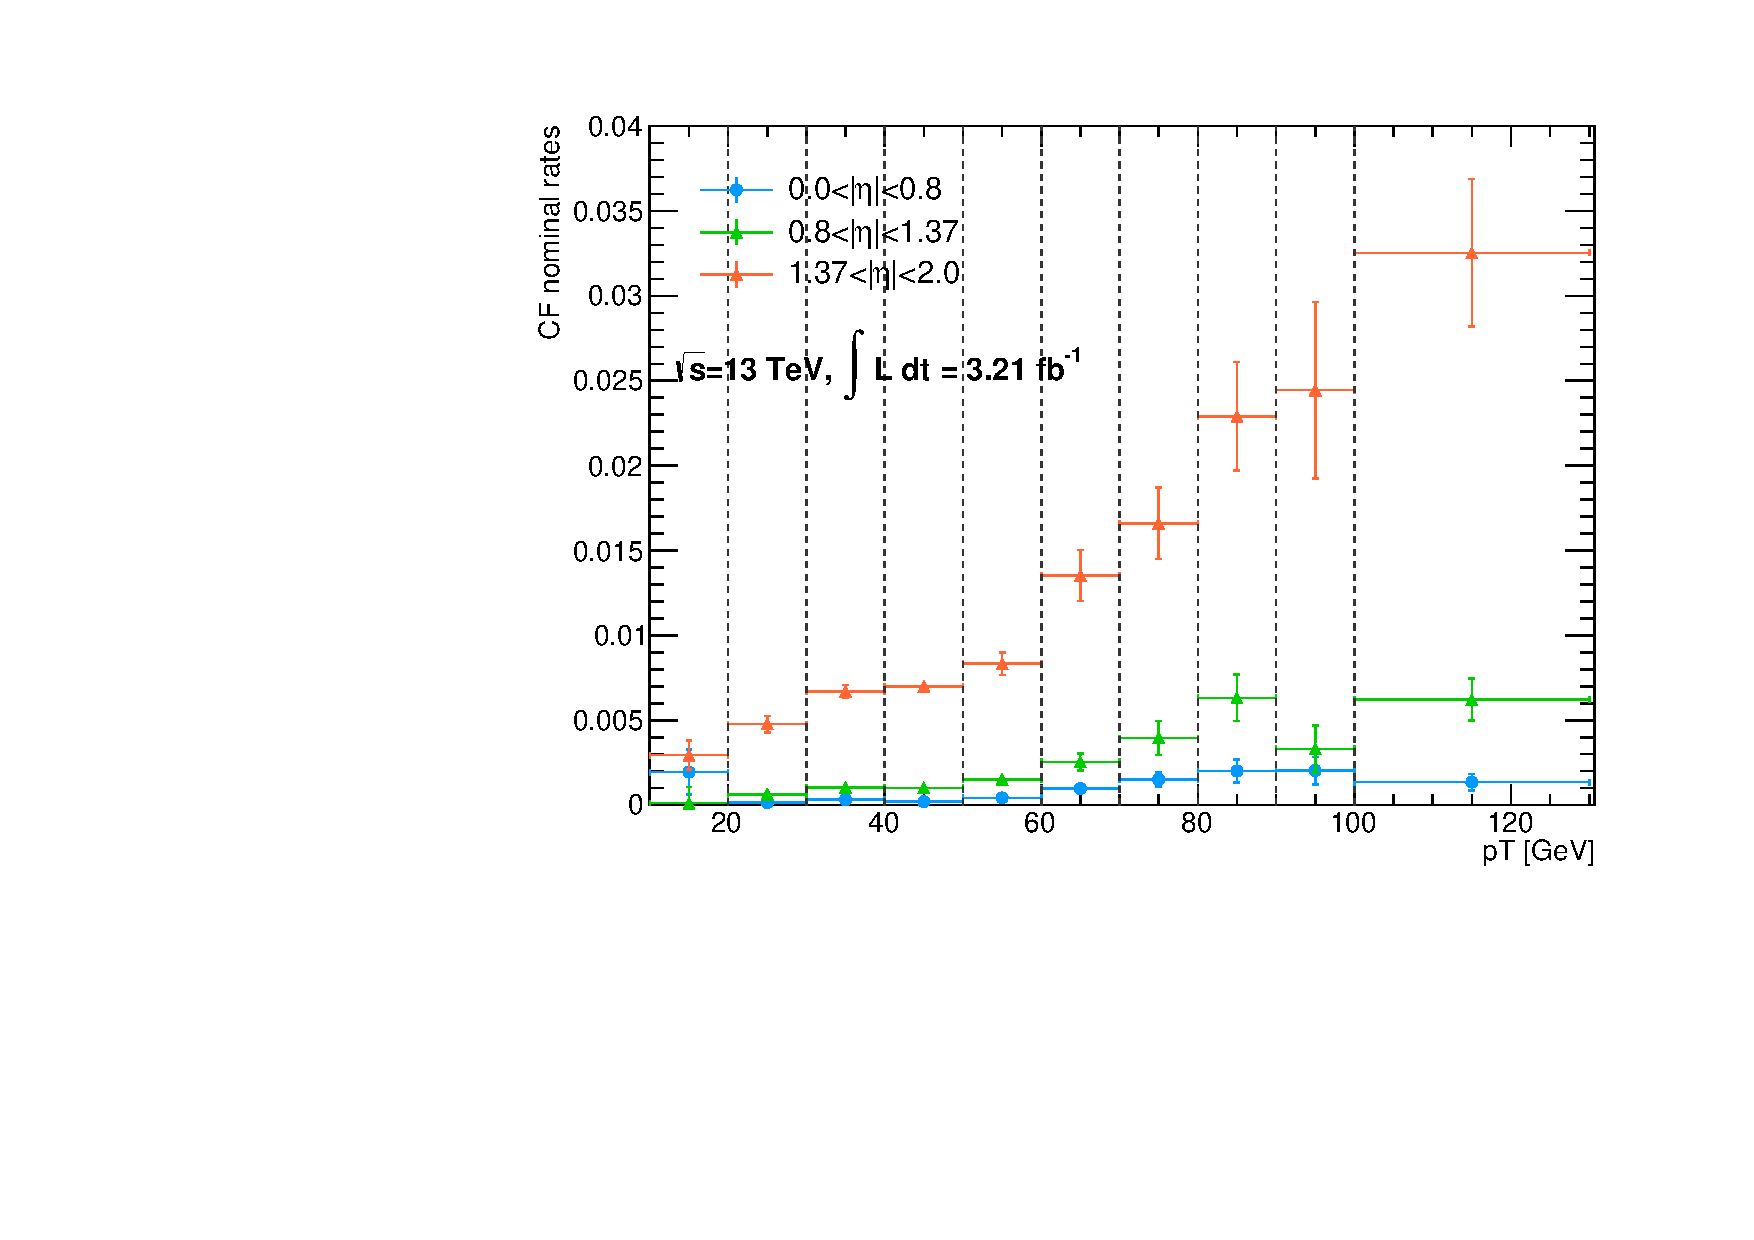
\includegraphics[width=\textwidth]{CFratesVSpt_data15}
	\caption{Data, signal electrons}\label{fig:Chflip_nominalData}
\end{subfigure}
\begin{subfigure}[b]{0.45\textwidth}
	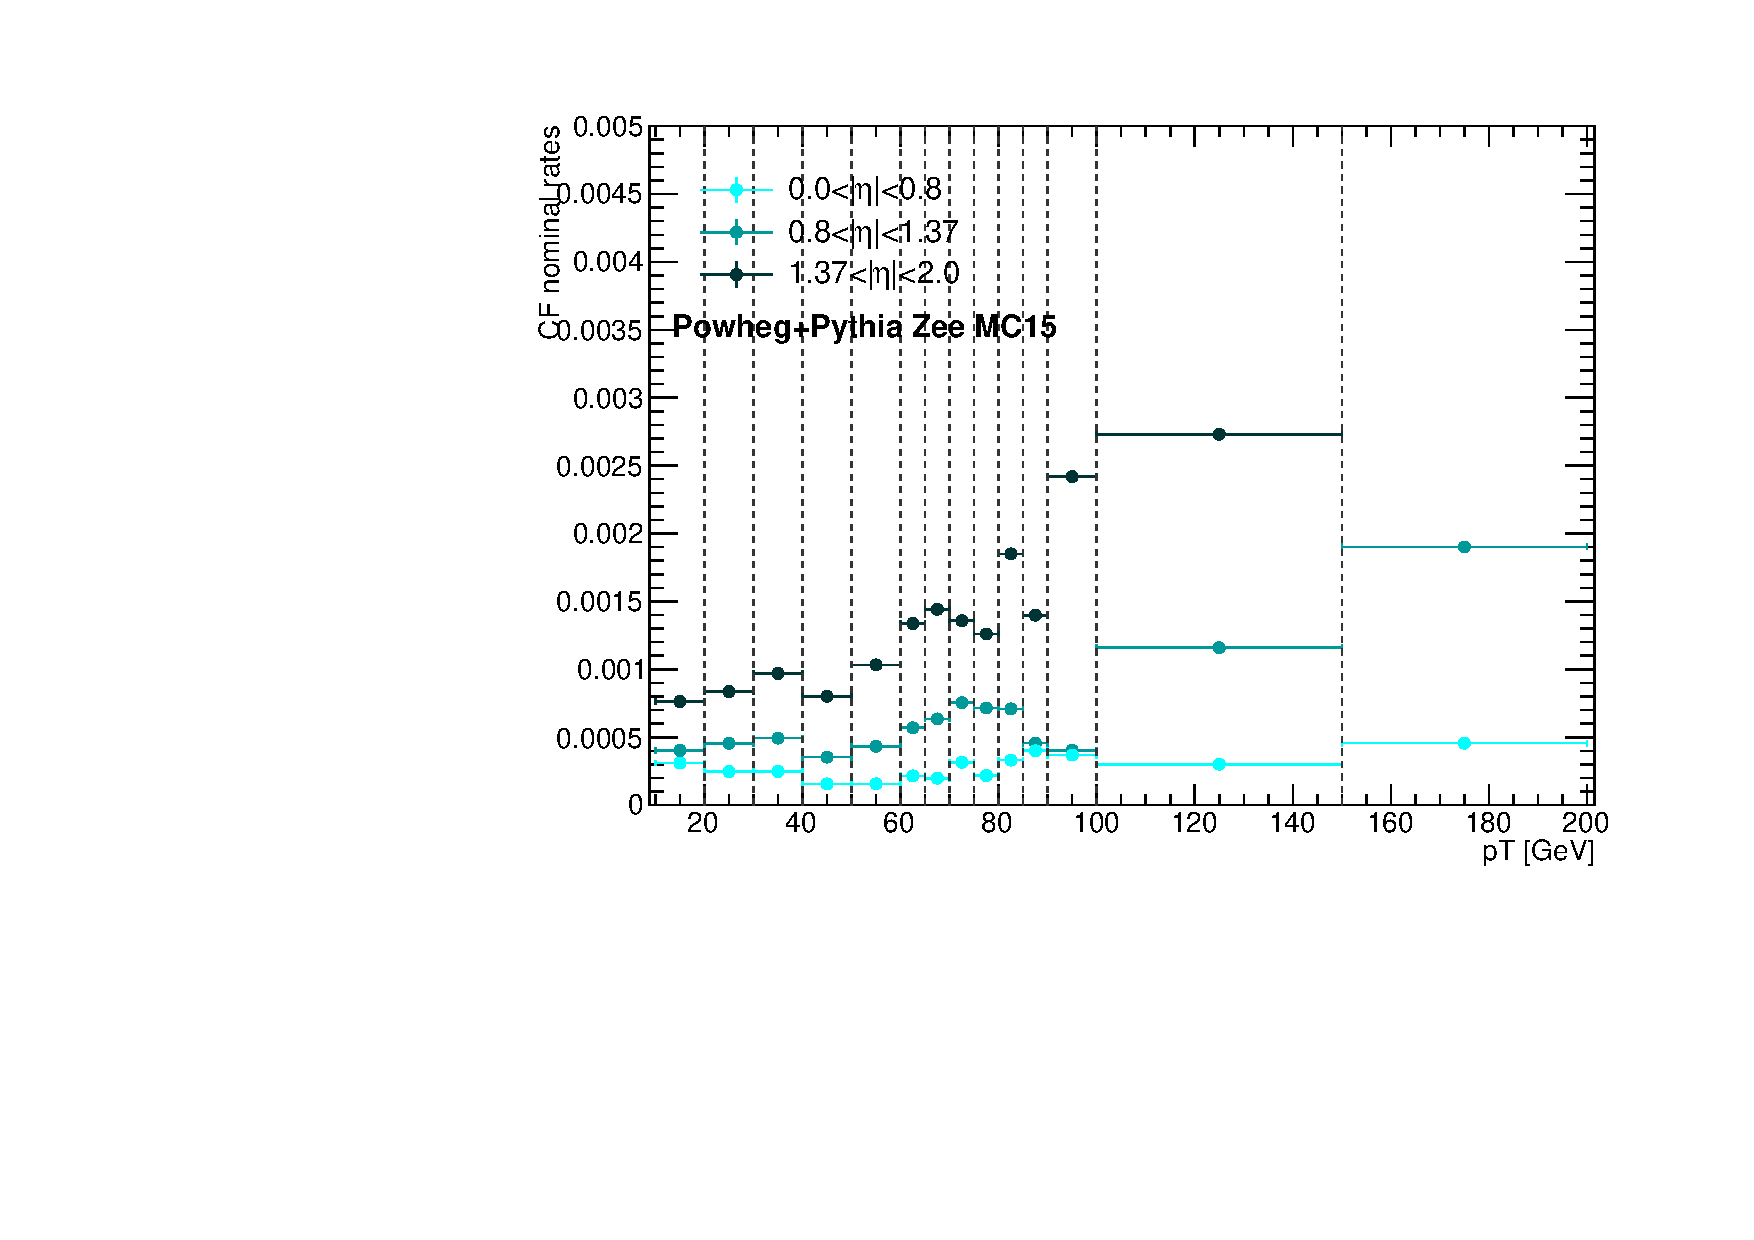
\includegraphics[width=\textwidth]{CFratesVSpt_MC15}
	\caption{MC, signal electrons}\label{fig:Chflip_nominalMC}
\end{subfigure}
\begin{subfigure}[b]{0.45\textwidth}
	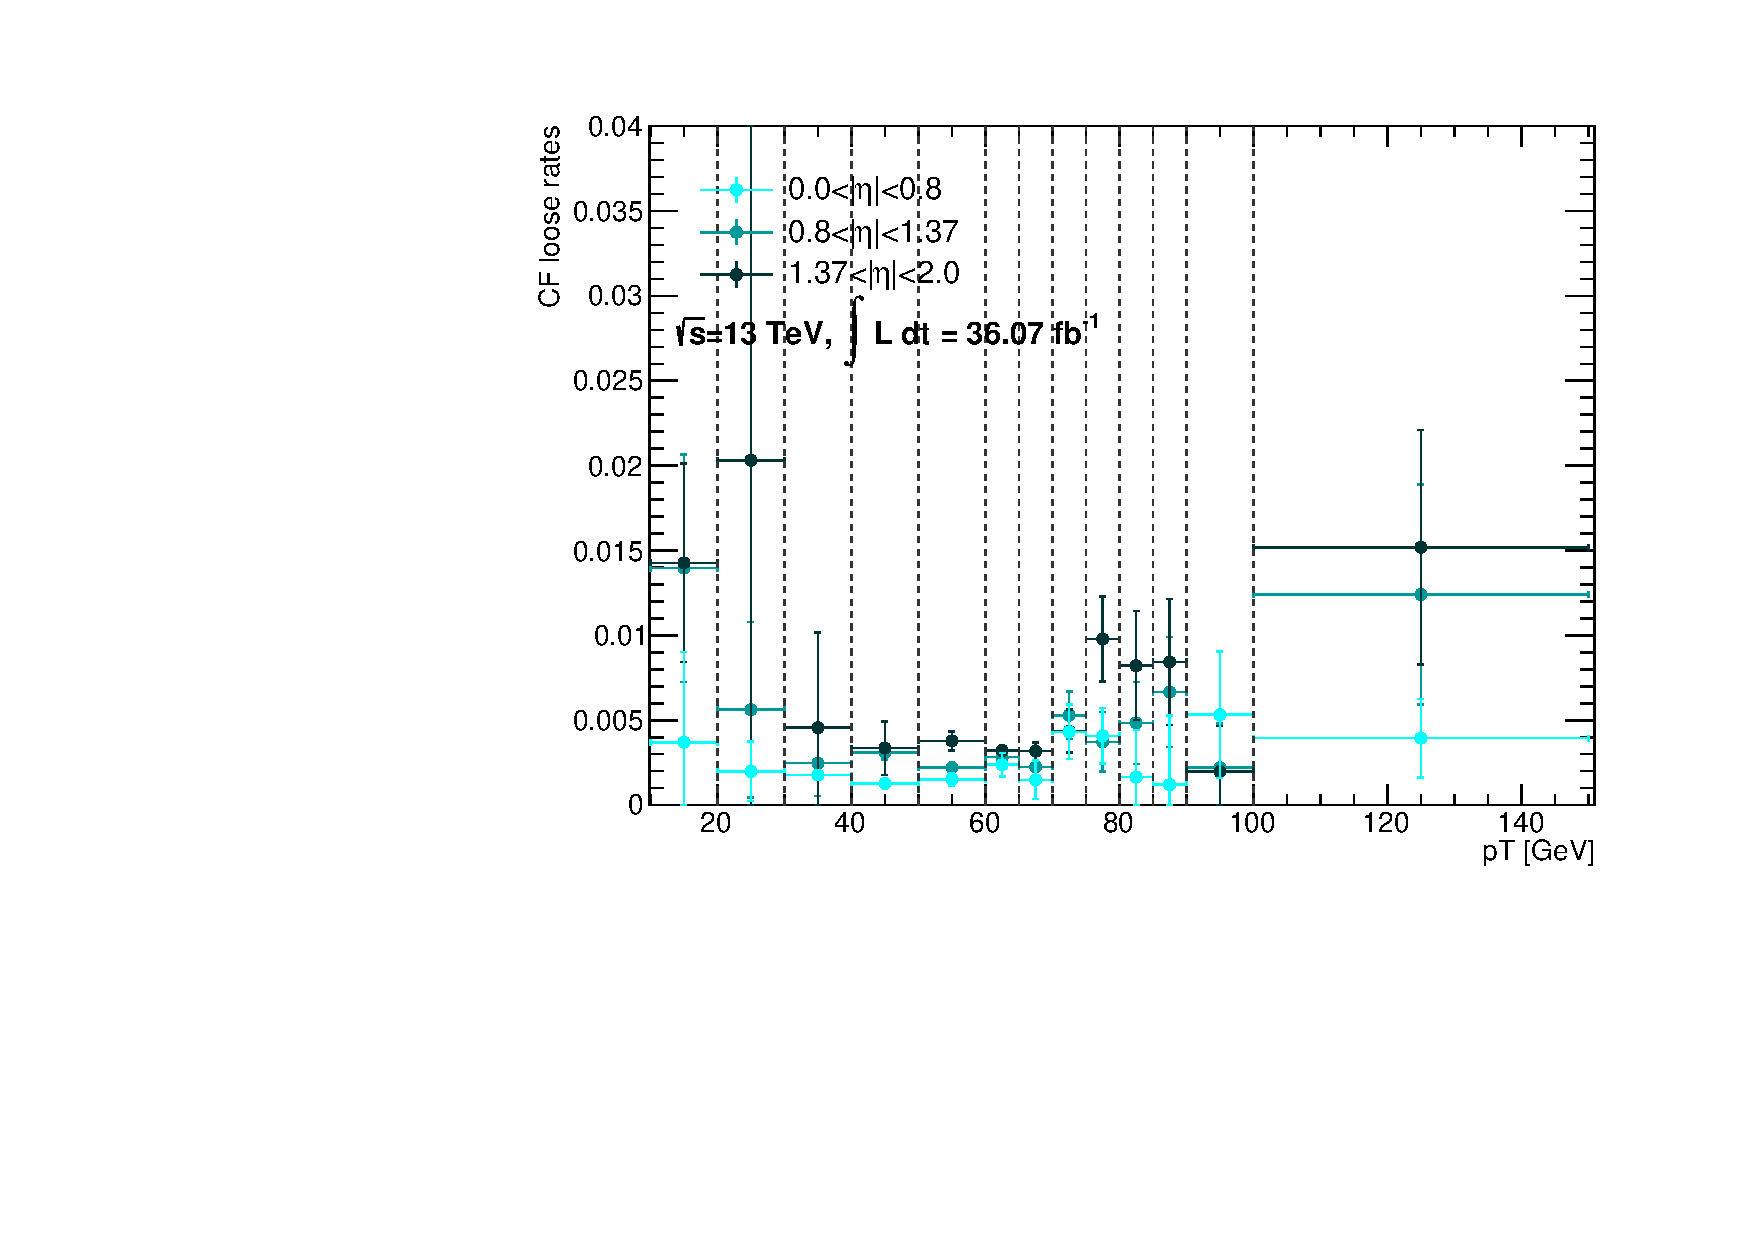
\includegraphics[width=\textwidth]{CFratesLOOSEVSpt_data15}
	\caption{Data, baseline-failing-signal}\label{fig:Chflip_looseData}
\end{subfigure}
\begin{subfigure}[b]{0.45\textwidth}
	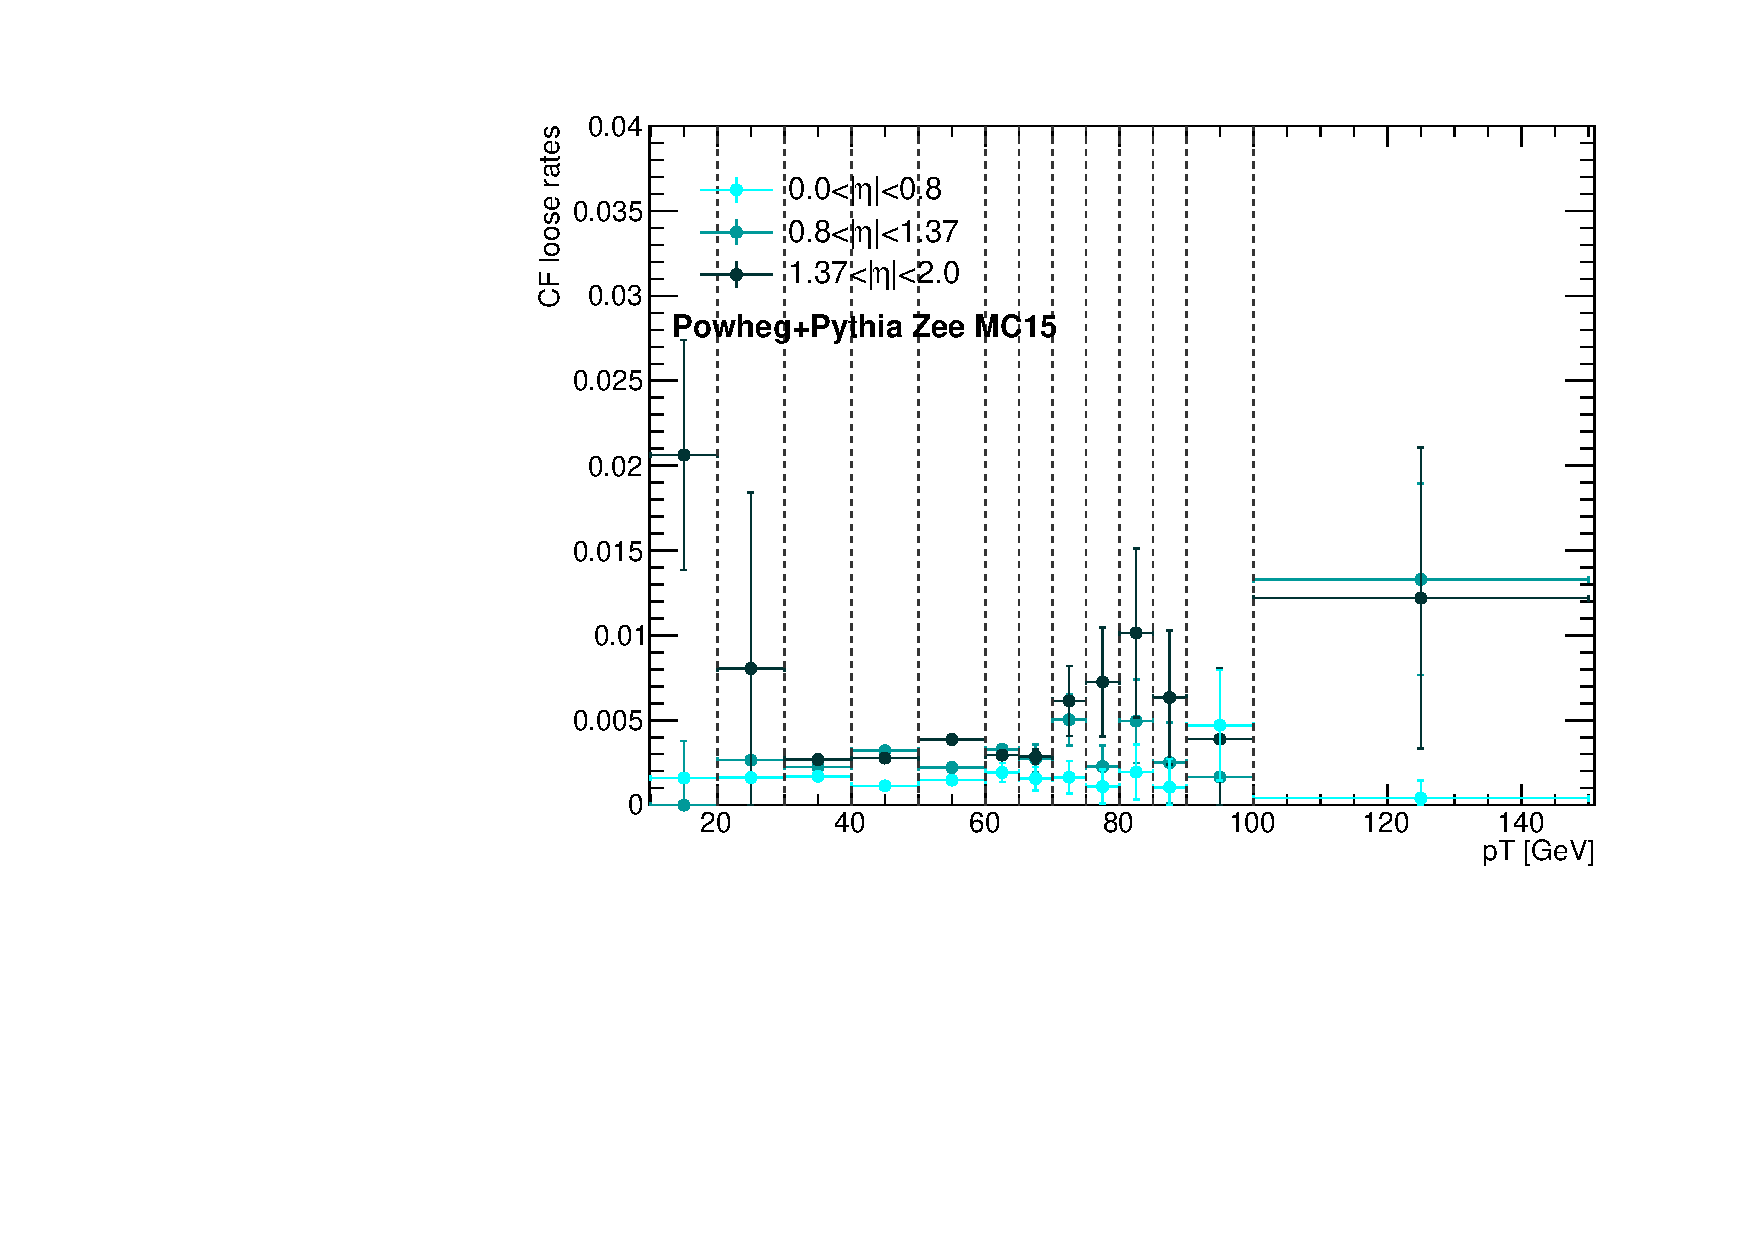
\includegraphics[width=\textwidth]{CFratesLOOSEVSpt_MC15}
	\caption{MC, baseline-failing-signal}\label{fig:Chflip_looseMC}
\end{subfigure}
\caption{Charge-flip rate as measured in data (left) and MC (right). 
Only the statistical uncertainty is displayed. The last \pt bin is inclusive.}
\label{fig:ChFlip_Rate}
\end{figure}

The charge-flip rates measured in data and MC are shown on Figure~\ref{fig:ChFlip_Rate}. 
 In data, the nominal rates (Fig.~\ref{fig:Chflip_nominalData}) go up to $\sim$0.1\% in the barrel region ($|\eta| < 1.37$), 
 while it increases up to $\sim$0.2\% in the end-cap region ($|\eta > 1.37|$). 
 For baseline electrons failing signal requirements (Fig.~\ref{fig:Chflip_looseData}), 
 the rates are in general greater than the nominal ones in every bin, as expected. The charge-flip rates for these electrons go up to $\sim$0.5\% in the barrel region and up 1\% in the end-cap region. Compared to the rates used in the previous version of the analysis~\cite{ATLAS-CONF-2016-037}, the central values are much lower now. After applying the \texttt{ElectronChargeIDSelector} tool, the charge flip rates are strongly reduced for both signal and baseline-failing-signal electrons (up to a factor 20 in some bins). Below 30 \GeV, the statistics is very low for the loose measurement; however, these results are used only to measure the electron fake rate and, as illustrated in Figure~\ref{Fig:fakes_preselection_electron}, in this \pt interval the charge flip background is negligible.
% while the statistical uncertainties decreased significantly given the increase of up to a factor three in data luminosity. 

The charge-flip rates in MC (Figs.~\ref{fig:Chflip_nominalMC},~\ref{fig:Chflip_looseMC}) 
are obtained by applying the same methodology as in data. 
Generally, the rates are not very far from data, validating the use of MC to predict charge-flip background 
in several of the optimization studies presented in this document. 
In addition, a closure test is performed on $t\bar t$ MC, 
checking that weighted OS events can reproduce the distribution of SS charge-flip events (identified by truth-matching). 
A good overall agreement is found, largely within the assigned uncertainties; 
detailed plots are included in appendix~\ref{app:chargeflip}. 

\subsection{Systematic uncertainties}
\label{subsec:chargeflip_uncertainties}

\begin{figure}[t!]
\centering
\begin{subfigure}[b]{0.75\textwidth}
	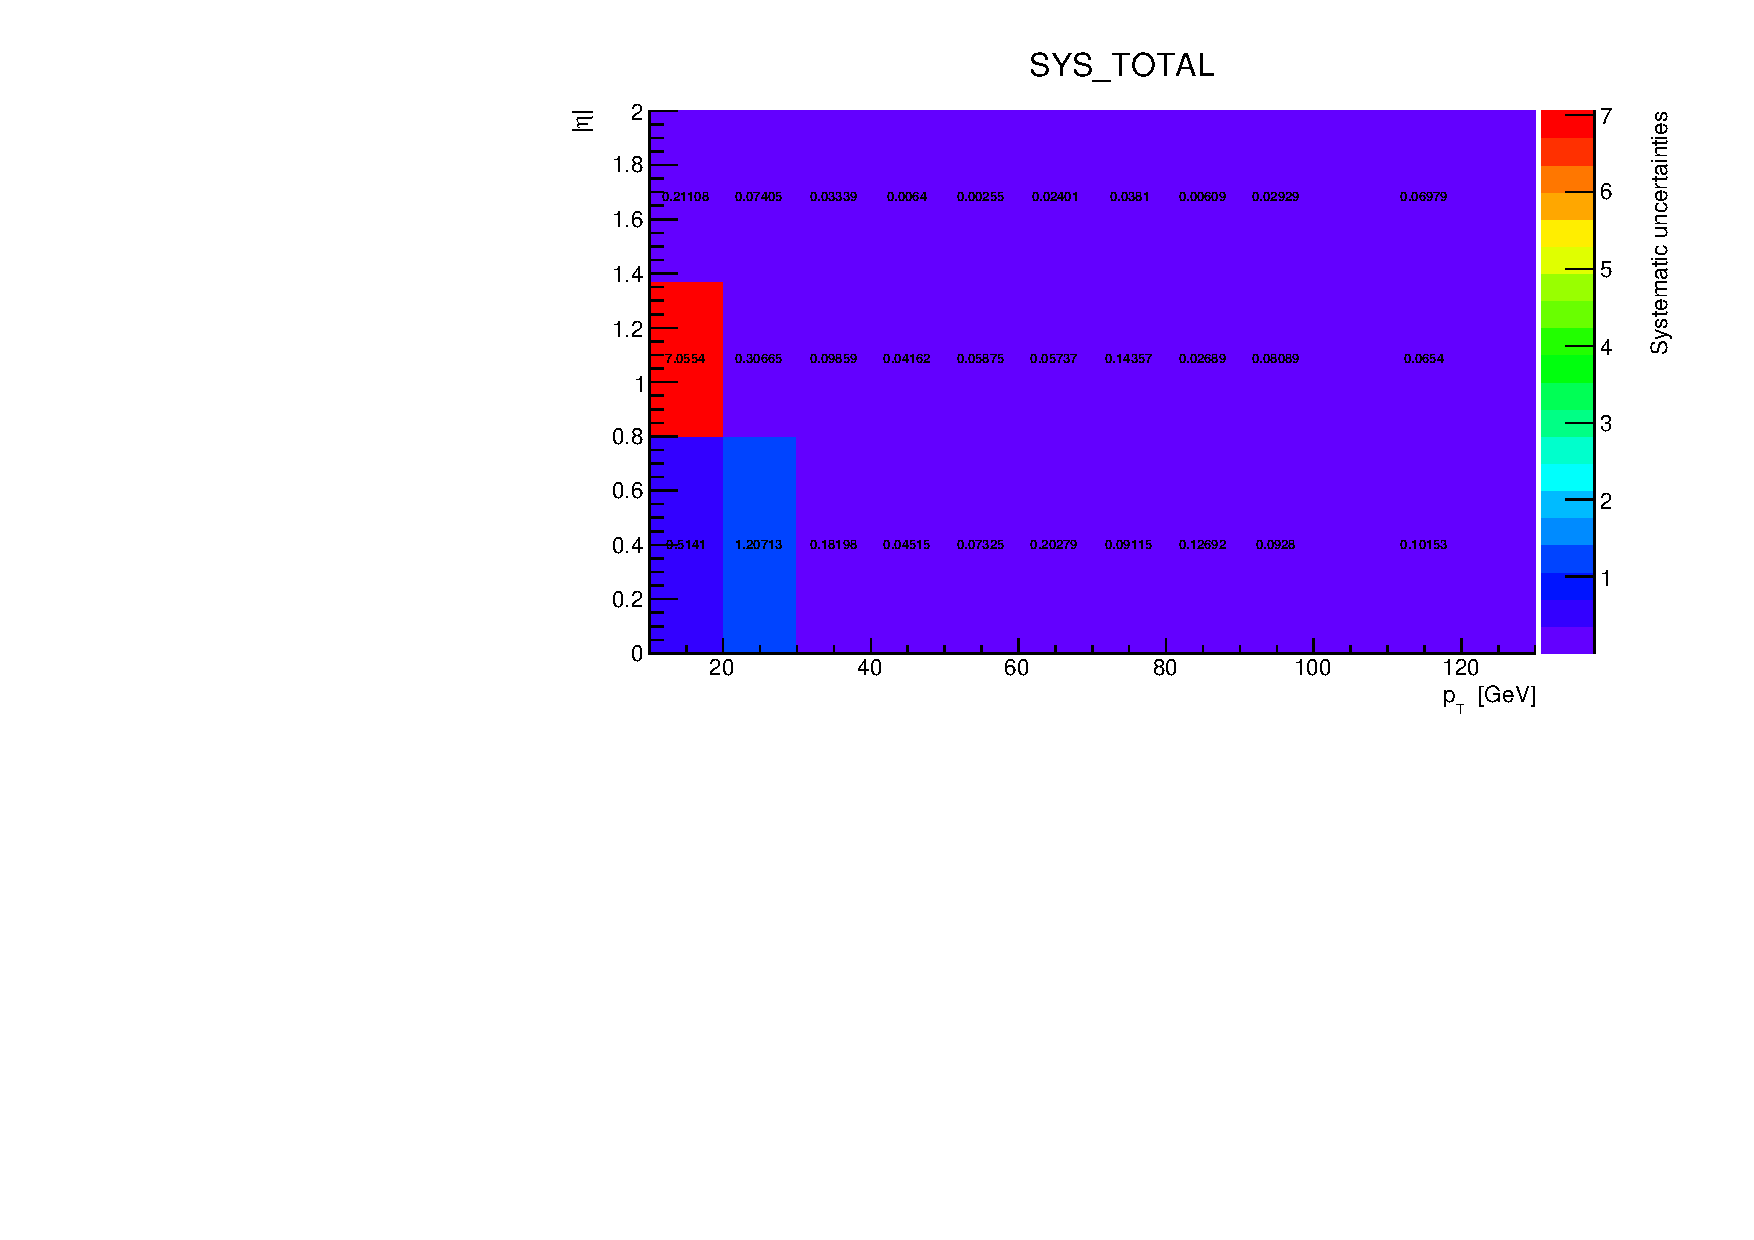
\includegraphics[width=\textwidth]{2D_histo_SYS_TOTAL}
\end{subfigure}
\begin{subfigure}[b]{0.75\textwidth}
	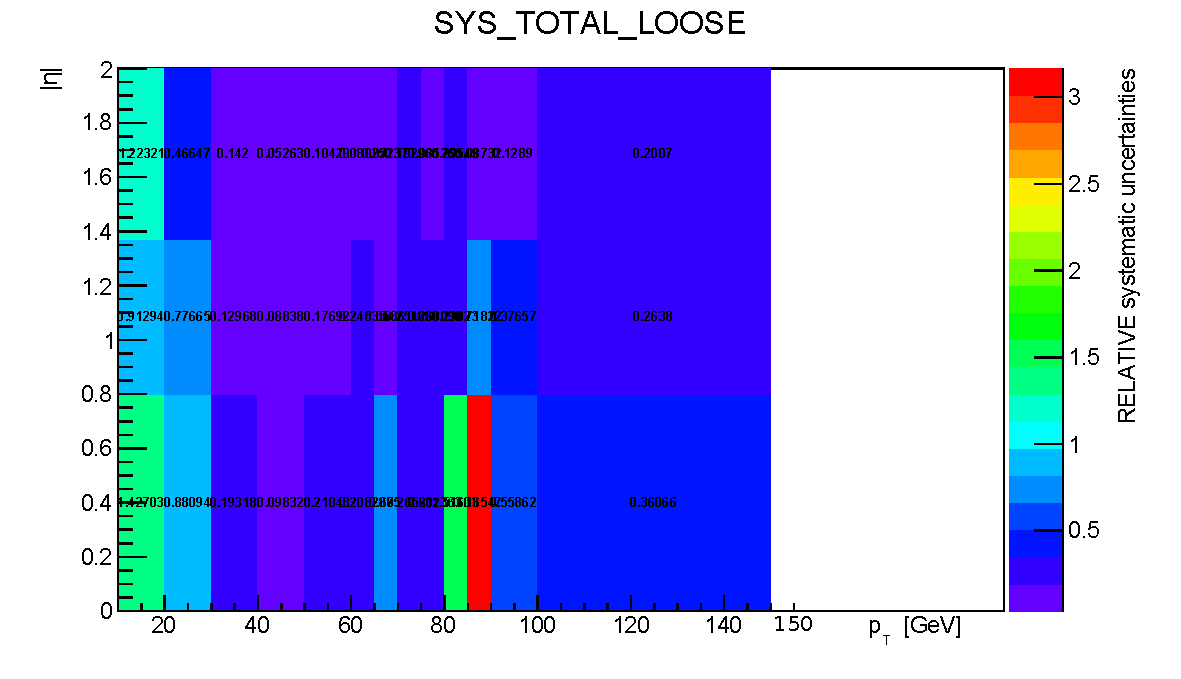
\includegraphics[width=\textwidth]{2D_histo_SYS_TOTAL_LOOSE}
\end{subfigure}
\caption{Total systematic uncertainties on the charge-flip rates for electrons satisfying the signal requirements (upper plot),
and for baseline electrons failing the signal requirements (lower plot). 
}
\label{fig:ChFlip_SYS_Total}
\end{figure}

The main uncertainties on the measured charge-flip rates come from the presence of background and the way it is estimated. To assess them, variations of the selection and background estimation are considered: 
\begin{itemize}
\item[1)] $75<m_{ee}<100 \GeV$, no background subtraction;
\item[2)] $75<m_{ee}<100 \GeV$, sidebands of 20 \GeV;
\item[3)] $75<m_{ee}<100 \GeV$, sidebands of 25 \GeV (nominal measurement);
\item[4)] $75<m_{ee}<100 \GeV$, sidebands of 30 \GeV;
\item[5)] $80<m_{ee}<100 \GeV$, sidebands of 20 \GeV.
\end{itemize}

The effect of applying the background subtraction itself is evaluated by comparing configurations 1 and 3. 
The impact of the width of the $m_{ee}$ chosen for the measurement is  by comparing configurations 3 and 5, 
while the sideband width effects are evaluated by comparing configuration 3 and 2, or 3 and 4. 
The largest deviation in each bin is taken as the systematic uncertainty on the charge-flip rate.

Those variations are shown in Appendix~\ref{app:chargeflip}~(Figs~\ref{fig:ChargeFlip_Syst_1}-\ref{fig:ChargeFlip_Syst_5}) for every bin. The resulting systematic uncertainties on the charge-flip rates are presented in Fig.~\ref{fig:ChFlip_SYS_Total}. 

For the signal electrons charge-flip rates the systematic uncertainties vary in general between 2\% and 20\% (increasing up to $>50\%$ in the region with $\pt < 10 \GeV$), whereas for baseline-failing-signal electrons they vary between 3\% and 30\% (increasing up to $>50\%$ in the region with $\pt < 10 \GeV$). Part of these large values, at low \pt and in the [80,90]~\GeV \pt interval, can be explained by large statistical fluctuations between the different configurations.



\subsection{Expected yields in signal regions}
\label{subsec:chargeflip_yields}

The expected background yields for processes with charge-flipped background, estimated with the method described in this section, 
are presented in Table~\ref{tab:chargeflip_sr_yields} for the signal regions. 
They are compared for illustration to the MC prediction for simulated \ttbar\ processes, and with the MC-template method (see section~\ref{subsec:fakes_mctemplate}). 
% The different estimates are consistent, and the predictions of the data-driven method described in this section are retained as the final estimate. 

\begin{table}[!htb]
\caption{Expected yields for background processes with charge-flipped electrons,
in the signal regions proposed in Section~\ref{sec:signalregions}, shown for 36 \ifb. 
Uncertainties include all statistical and systematic sources. 
Charge-flip processes do not contribute to signal regions which require $\ge 3$ leptons. 
For illustration, charge-flip yields obtained with the MC-template method (section~\ref{subsec:fakes_mctemplate}) are compared to the data-driven estimate. 
}
\label{tab:chargeflip_sr_yields}
\centering
\begin{tabular}{|c||c|c|}\hline
 Region      &   Weighted OS data          &     Template method \\\hline
    Rpc2L0bH & $ 0.01 \pm  0.00 \pm  0.00$ & $<0.4$ \\
    Rpc2L0bS & $ 0.05 \pm  0.01 \pm  0.01$ & $ 00.02 \pm 00.02 \pm 00.00 $ \\
    Rpc2L1bH & $ 0.25 \pm  0.03 \pm  0.04$ & $ 00.21 \pm 00.32 \pm 00.16 $ \\
    Rpc2L1bS & $ 0.25 \pm  0.02 \pm  0.04$ & $ 00.35 \pm 00.37 \pm 00.26 $ \\
    Rpc2L2bH & $ 0.02 \pm  0.01 \pm  0.00$ & $<0.4$ \\
    Rpc2L2bS & $ 0.10 \pm  0.01 \pm  0.02$ & $<0.4$ \\
 Rpc2Lsoft1b & $ 0.08 \pm  0.01 \pm  0.02$ & $<0.4$ \\
 Rpc2Lsoft2b & $ 0.08 \pm  0.01 \pm  0.02$ & $<0.4$ \\
   Rpc3LSS1b & $ 0.39 \pm  0.03 \pm  0.07$ & $ 00.81 \pm 00.53 \pm 00.34 $ \\
     Rpv2L0b & $ 0.03 \pm  0.02 \pm  0.00$ & $ 00.22 \pm 00.06 \pm 00.09 $ \\
    Rpv2L1bH & $ 0.02 \pm  0.01 \pm  0.00$ & $ 00.02 \pm 00.01 \pm 00.01 $ \\
    Rpv2L1bM & $ 0.10 \pm  0.01 \pm  0.02$ & $ 00.10 \pm 00.06 \pm 00.04 $ \\
    Rpv2L1bS & $ 0.74 \pm  0.04 \pm  0.11$ & $ 01.30 \pm 00.66 \pm 00.54 $ \\
    Rpv2L2bH & $ 0.03 \pm  0.01 \pm  0.01$ & $<0.4$ \\
    Rpv2L2bS & $ 0.46 \pm  0.03 \pm  0.07$ & $ 01.55 \pm 01.07 \pm 01.25 $ \\
\hline
\hline
\end{tabular}
\end{table}


\subsection{Expected yields in signal regions}
\label{subsec:fakes_yields}

The expected yield for processes with fake leptons, 
estimated with the method described in sections~\ref{subsec:fakes_matrix} and~\ref{subsec:fakes_mctemplate}, 
are presented in Table~\ref{tab:fakes_sr_yields} for the signal regions. 
They are compared for cross-check with the alternative ABCD prediction (section~\ref{subsec:fakes_abcd}), 
and are all found to be consistent with each other. 

The final numbers retained for the fake lepton background estimate (also shown in the tables) 
are taken as the weighted-average of the predictions from the matrix method and the MC template; 
the weights are based on the statistical component, and the systematic uncertainties are propagated 
assuming conservatively a full correlation between the two methods (although they are in fact largely independent!). 
The central value and statistical/systematic uncertainties are therefore: 

\begin{align}
&\left(w\zeta_1 + (1-w)\zeta_2\right) 
\pm \sqrt{w^2\left(\Delta\zeta_1^\text{(stat)}\right)^2 + (1-w)^2\left(\Delta\zeta_2^\text{(stat)}\right)^2} 
\pm \left(w\Delta\zeta_1^\text{(syst)} + (1-w)\Delta\zeta_2^\text{(syst)}\right)\\
&\qquad\text{ with }w=\frac{\left(\Delta\zeta_2^\text{(stat)}\right)^2}{\left(\Delta\zeta_1^\text{(stat)}\right)^2+\left(\Delta\zeta_2^\text{(stat)}\right)^2}\notag
\end{align}

When the estimated value is too small(below 0.15), the expected yield is set to $0.15\pm 0.15$, 
to cover for possibilities of an under-fluctuation of the number of baseline-not-signal leptons 
when applying the matrix method, as well as lack of statistics in the MC samples for the other method. 
 
This upper bound is inflated if the original combined prediction $x\pm\Delta x$ 
is such that its plus-one-sigma variation exceeds the upper bound, that is $\delta=(x+\Delta x)>0.30$; 
in that case the final retained number is $(\delta/2)\pm (\delta/2)$. 
There is no such instance in the current SR estimates, though, as can be seen in the table.  

\begin{table}[!htb]
\caption{Expected yields for background processes with fake leptons,
in the signal regions proposed in Section~\ref{sec:signalregions}, shown for 36 \ifb. 
Uncertainties include all statistical and systematic sources for the nominal estimate (except ABCD, cf section~\ref{subsec:fakes_abcd}). 
}
\label{tab:fakes_sr_yields}
\centering
\resizebox{\textwidth}{!}{
\begin{tabular}{|c||c|c|c||c|}\hline
      Region &              Matrix method   &   Template method   &       ABCD method   &     Retained estimate  \\\hline
% v52, updated uncertainties and real efficiencies
    Rpc2L0bH & $ 0.83 \pm  0.56 \pm  0.74$  &  $1.00 \pm 0.96 \pm 0.81$  &  $0.36\pm 0.25 \pm 0.06$   &  $ 0.87 \pm  0.48 \pm  0.76$  \\
    Rpc2L0bS & $ 1.51 \pm  0.60 \pm  0.66$  &  $1.68 \pm 1.02 \pm 1.26$  &  $0.66\pm 0.39\pm 0.22$    &  $ 1.55 \pm  0.52 \pm  0.81$  \\
    Rpc2L1bH & $ 3.54 \pm  1.62 \pm  3.12$  &  $2.07 \pm 0.63 \pm 1.56$  &  $2.06\pm 0.32\pm 0.16$    &  $ 2.26 \pm  0.59 \pm  1.76$  \\
    Rpc2L1bS & $ 2.65 \pm  1.21 \pm  1.89$  &  $02.33 \pm 01.17 \pm 02.10$  &   $2.7\pm 0.6\pm 1.5$     &  $ 2.48 \pm  0.84 \pm  2.00$  \\ 
    Rpc2L2bH & $-0.11 \pm  0.11 \pm  0.18$  &  $<0.5$  &  $0.10\pm 0.05\pm 0.03$    &  $ 0.15 \pm  0.15 \pm  0.00$  \\
    Rpc2L2bS & $ 1.31 \pm  1.07 \pm  1.65$  &  $0.41 \pm 0.33 \pm 0.45$  &  $1.1\pm 0.2\pm 0.4$       &  $ 0.49 \pm  0.32 \pm  0.55$  \\
    Rpc2Lsoft1b & $ 4.75 \pm  1.42 \pm  2.64$  &  $2.48 \pm 1.32 \pm 1.86$  &  $1.2\pm 0.3\pm 1.2$       &  $ 3.53 \pm  0.97 \pm  2.22$  \\
    Rpc2Lsoft2b & $ 1.91 \pm  1.18 \pm  1.63$  &  $1.66 \pm 0.66 \pm 1.28$  &  $0.72\pm 0.19\pm 0.26$    &  $ 1.72 \pm  0.58 \pm  1.36$  \\
    Rpc3L0bH & $-0.01 \pm  0.11 \pm  0.10$  &  $<0.5$  &  $<0$                      &  $ 0.15 \pm  0.15 \pm  0.00$  \\
    Rpc3L0bS & $ 2.31 \pm  1.50 \pm  2.63$  &  $0.21 \pm 0.15 \pm 0.16$  &  $<0$                      &  $ 0.23 \pm  0.15 \pm  0.18$  \\
    Rpc3L1bH & $ 0.57 \pm  0.43 \pm  0.50$  &  $0.42 \pm 0.29 \pm 0.32$  &  $<0$                      &  $ 0.47 \pm  0.24 \pm  0.38$  \\
    Rpc3L1bS & $ 4.94 \pm  1.83 \pm  2.96$  &  $3.55 \pm 1.80 \pm 2.76$  &  $1.0\pm 0.9\pm 0.1$       &  $ 4.23 \pm  1.28 \pm  2.86$  \\
    Rpc3LSS1b & $-0.18 \pm  1.24 \pm  2.85$  &  $0.90 \pm 0.14 \pm 0.69$  &  $-$                       &  $ 0.89 \pm  0.14 \pm  0.72$  \\
    Rpv2L0b & $ 0.14 \pm  0.22 \pm  0.27$  &  $1.02 \pm 0.96 \pm 0.76$  &  $0.13\pm 0.12\pm 0.04$    &  $ 0.18 \pm  0.21 \pm  0.29$  \\
    Rpv2L1bH & $-0.06 \pm  0.03 \pm  0.09$  &  $0.60 \pm 0.35 \pm 0.48$  &  $0.31\pm 0.11\pm 0.08$    &  $ 0.15 \pm  0.15 \pm  0.00$  \\
    Rpv2L1bM & $ 1.70 \pm  2.07 \pm  1.68$  &  $1.20 \pm 0.69 \pm 0.95$  &  $0.53\pm 0.10\pm 0.18$    &  $ 1.25 \pm  0.65 \pm  1.02$  \\
    Rpv2L1bS & $16.49 \pm  4.04 \pm 18.70$  &  $4.46 \pm 1.67 \pm 3.45$  &  $4.5\pm 0.9\pm 1.4$       &  $ 6.22 \pm  1.54 \pm  5.68$  \\
    Rpv2L2bH & $-0.04 \pm  0.02 \pm  0.04$  &  $<0.5$  &  $0.26\pm 0.08 \pm 0.07$   &  $ 0.15 \pm  0.15 \pm  0.00$  \\
    Rpv2L2bS & $ 9.67 \pm  3.29 \pm  9.04$  &  $7.24 \pm 2.36 \pm 5.43$  &  $2.7\pm 0.5\pm 1.0$       &  $ 8.07 \pm  1.92 \pm  6.66$  \\	  
\hline
\hline
\end{tabular}
}
\end{table}

To check the validity and robustness of the FNP lepton estimate, 
the distributions of several discriminating variables in data are compared 
with the predicted background after various requirements on the number of jets and $b$-jets. 
Examples of such distributions are shown in Figure~\ref{fig:Bkg_distribs}, 
and illustrate that the data are described by the prediction within uncertainties. The apparent disagreement 
for \meff\ above 1 TeV in Figure~\ref{fig:VRmeff2} is covered by the large theory uncertainty for the diboson background, which is not shown 
but amounts to about 30\% for \meff\ above 1 TeV.

\begin{figure}[th!]
\centering
\begin{subfigure}[t]{0.49\textwidth}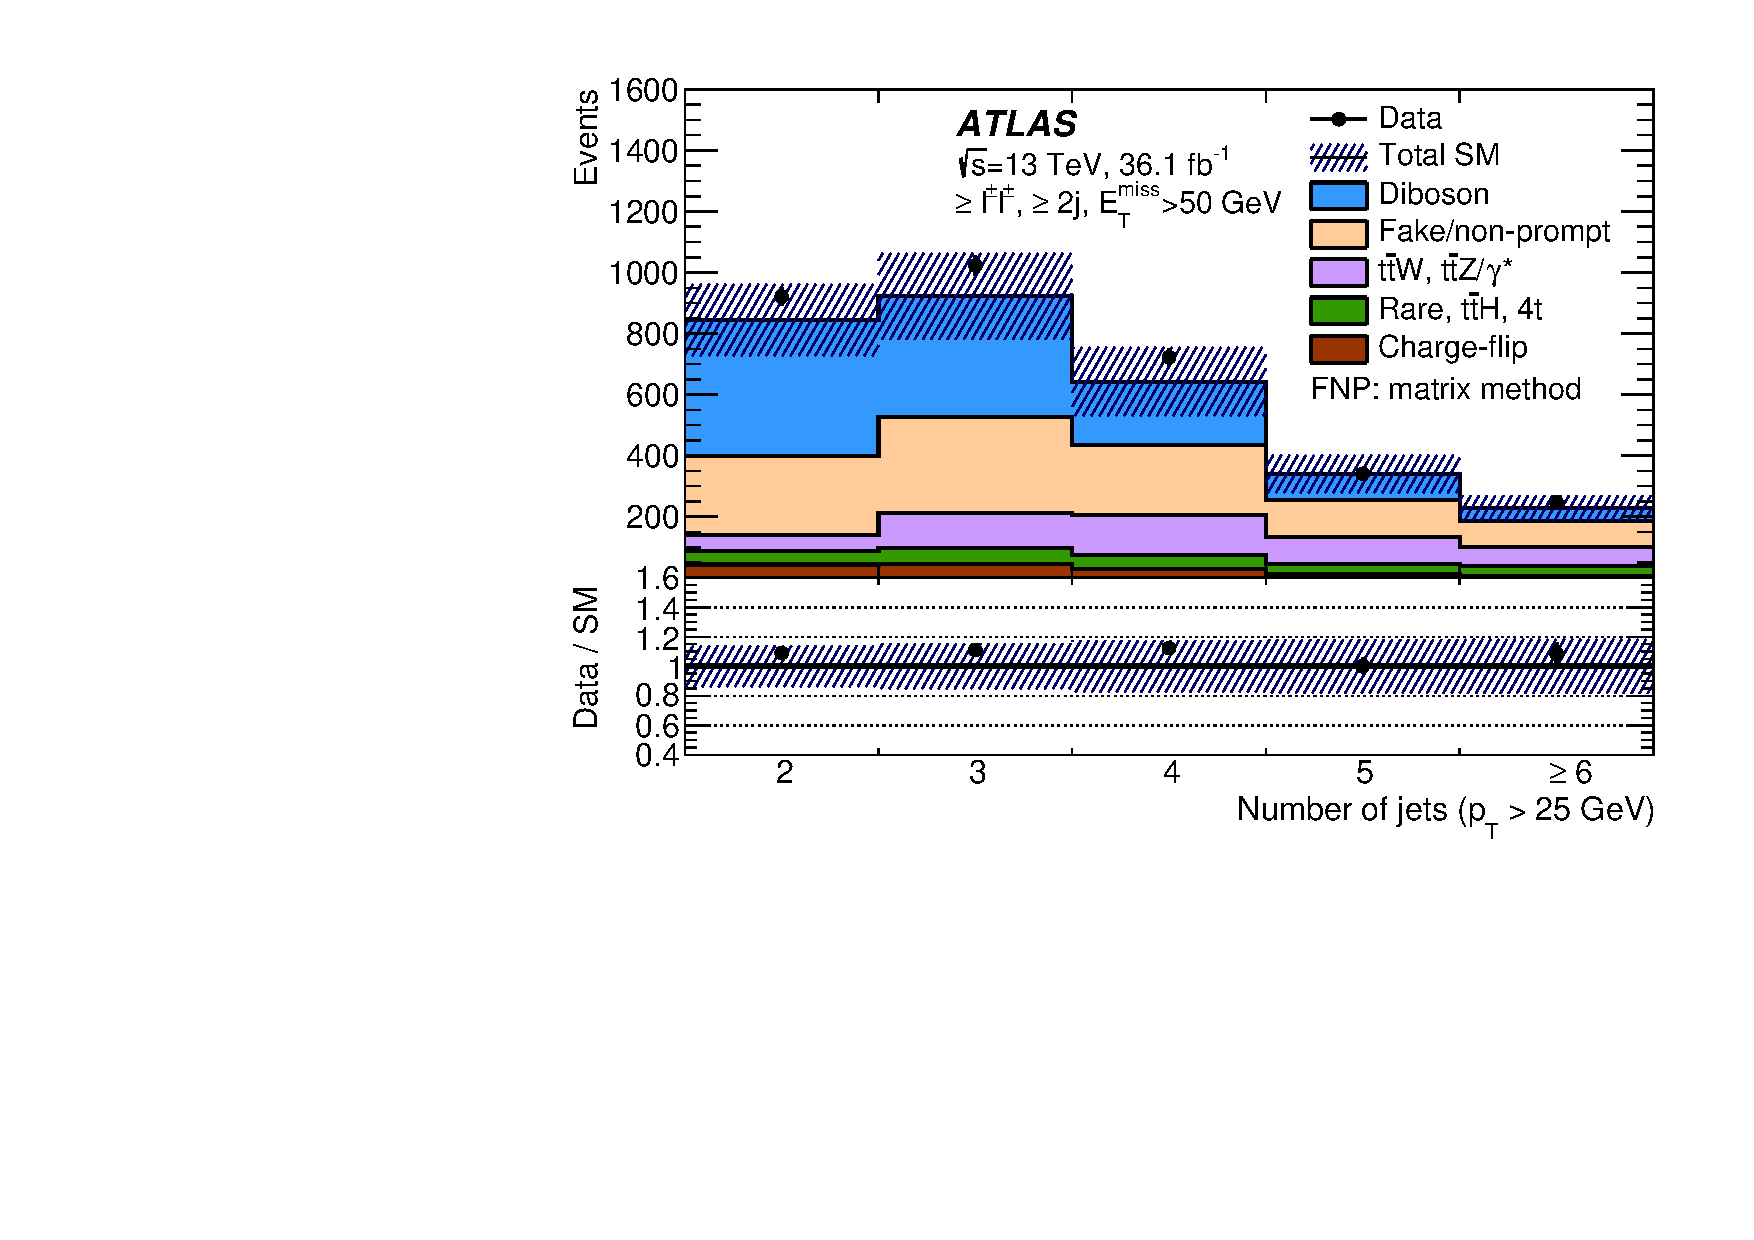
\includegraphics[width=\textwidth]{PAPER_DILEP_2JMET50_njets25}\caption{}\label{fig:VRnj}\end{subfigure}
\begin{subfigure}[t]{0.49\textwidth}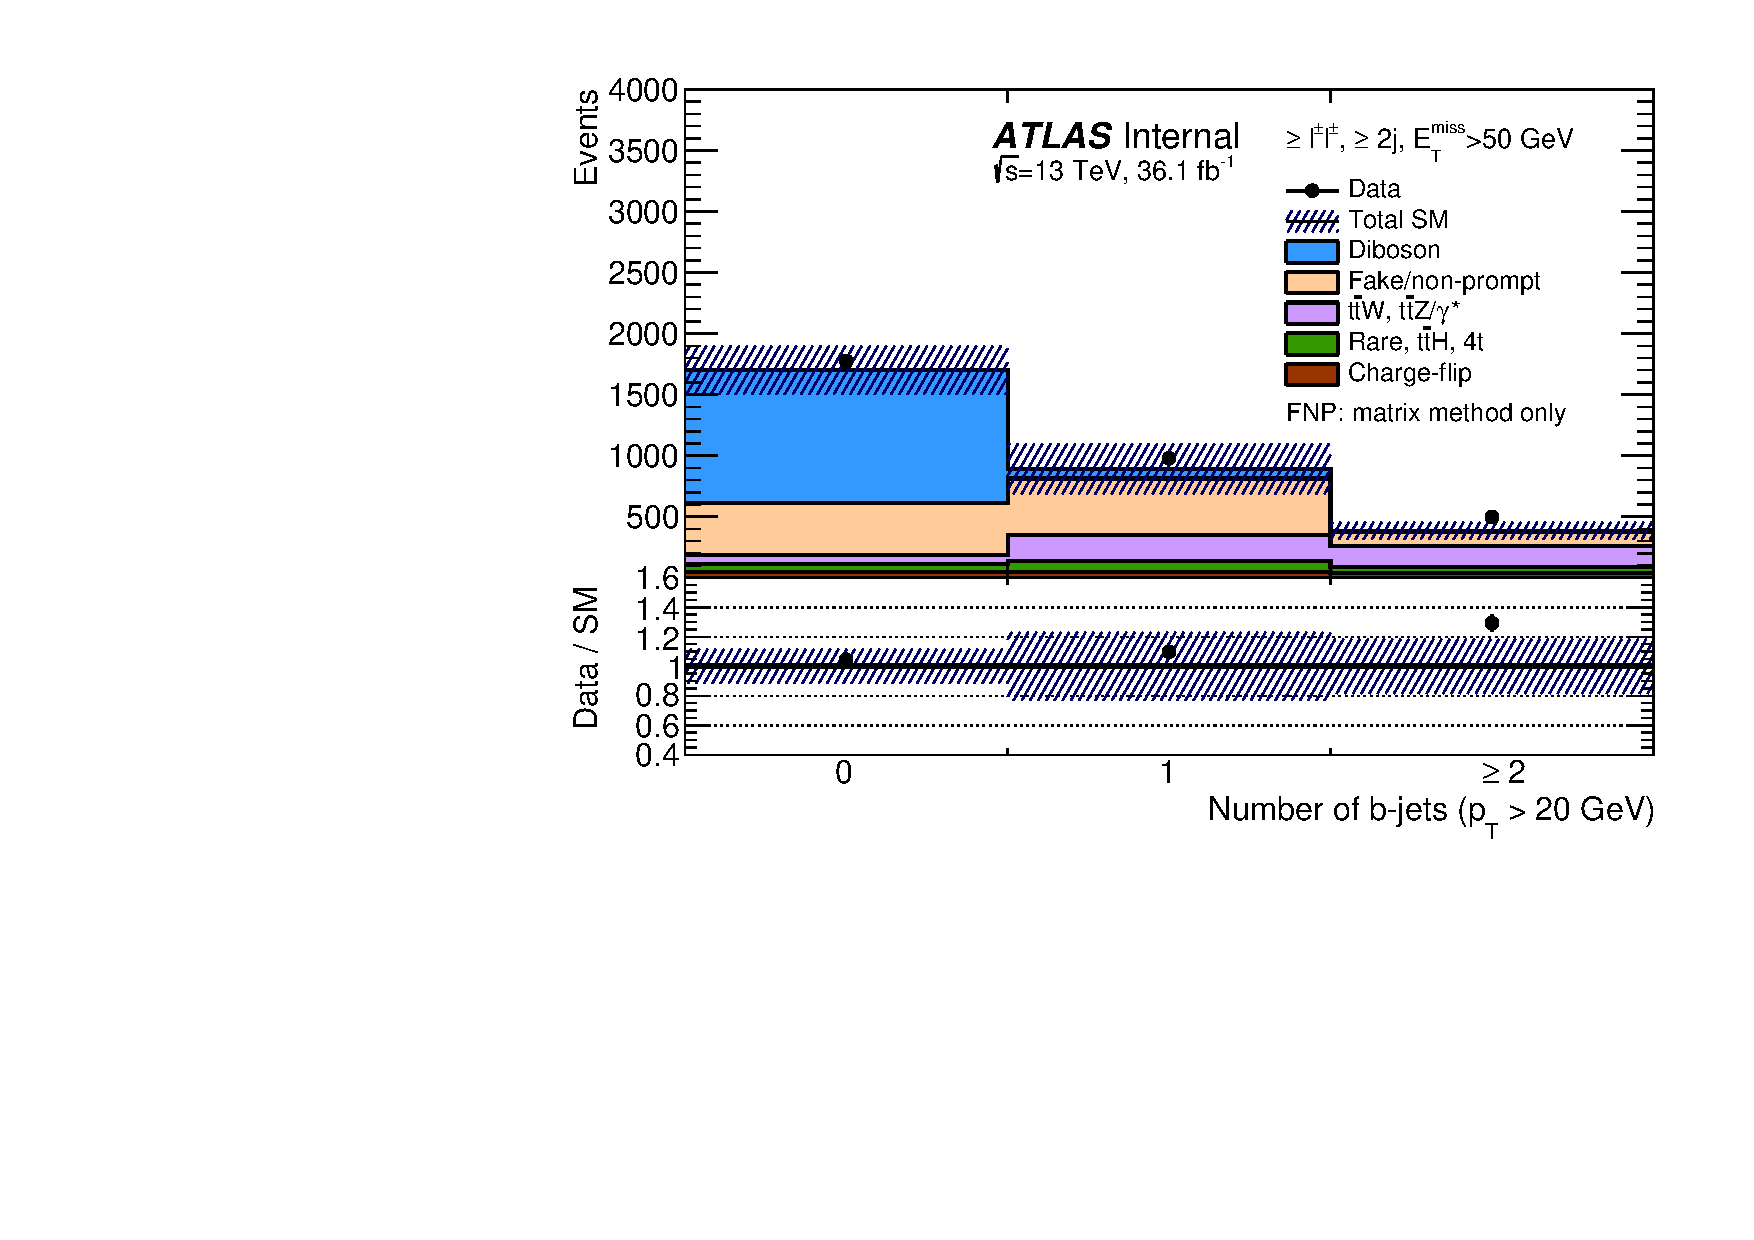
\includegraphics[width=\textwidth]{PAPER_DILEP_2JMET50_nbjets}\caption{}\label{fig:VRnb}\end{subfigure}
\begin{subfigure}[t]{0.49\textwidth}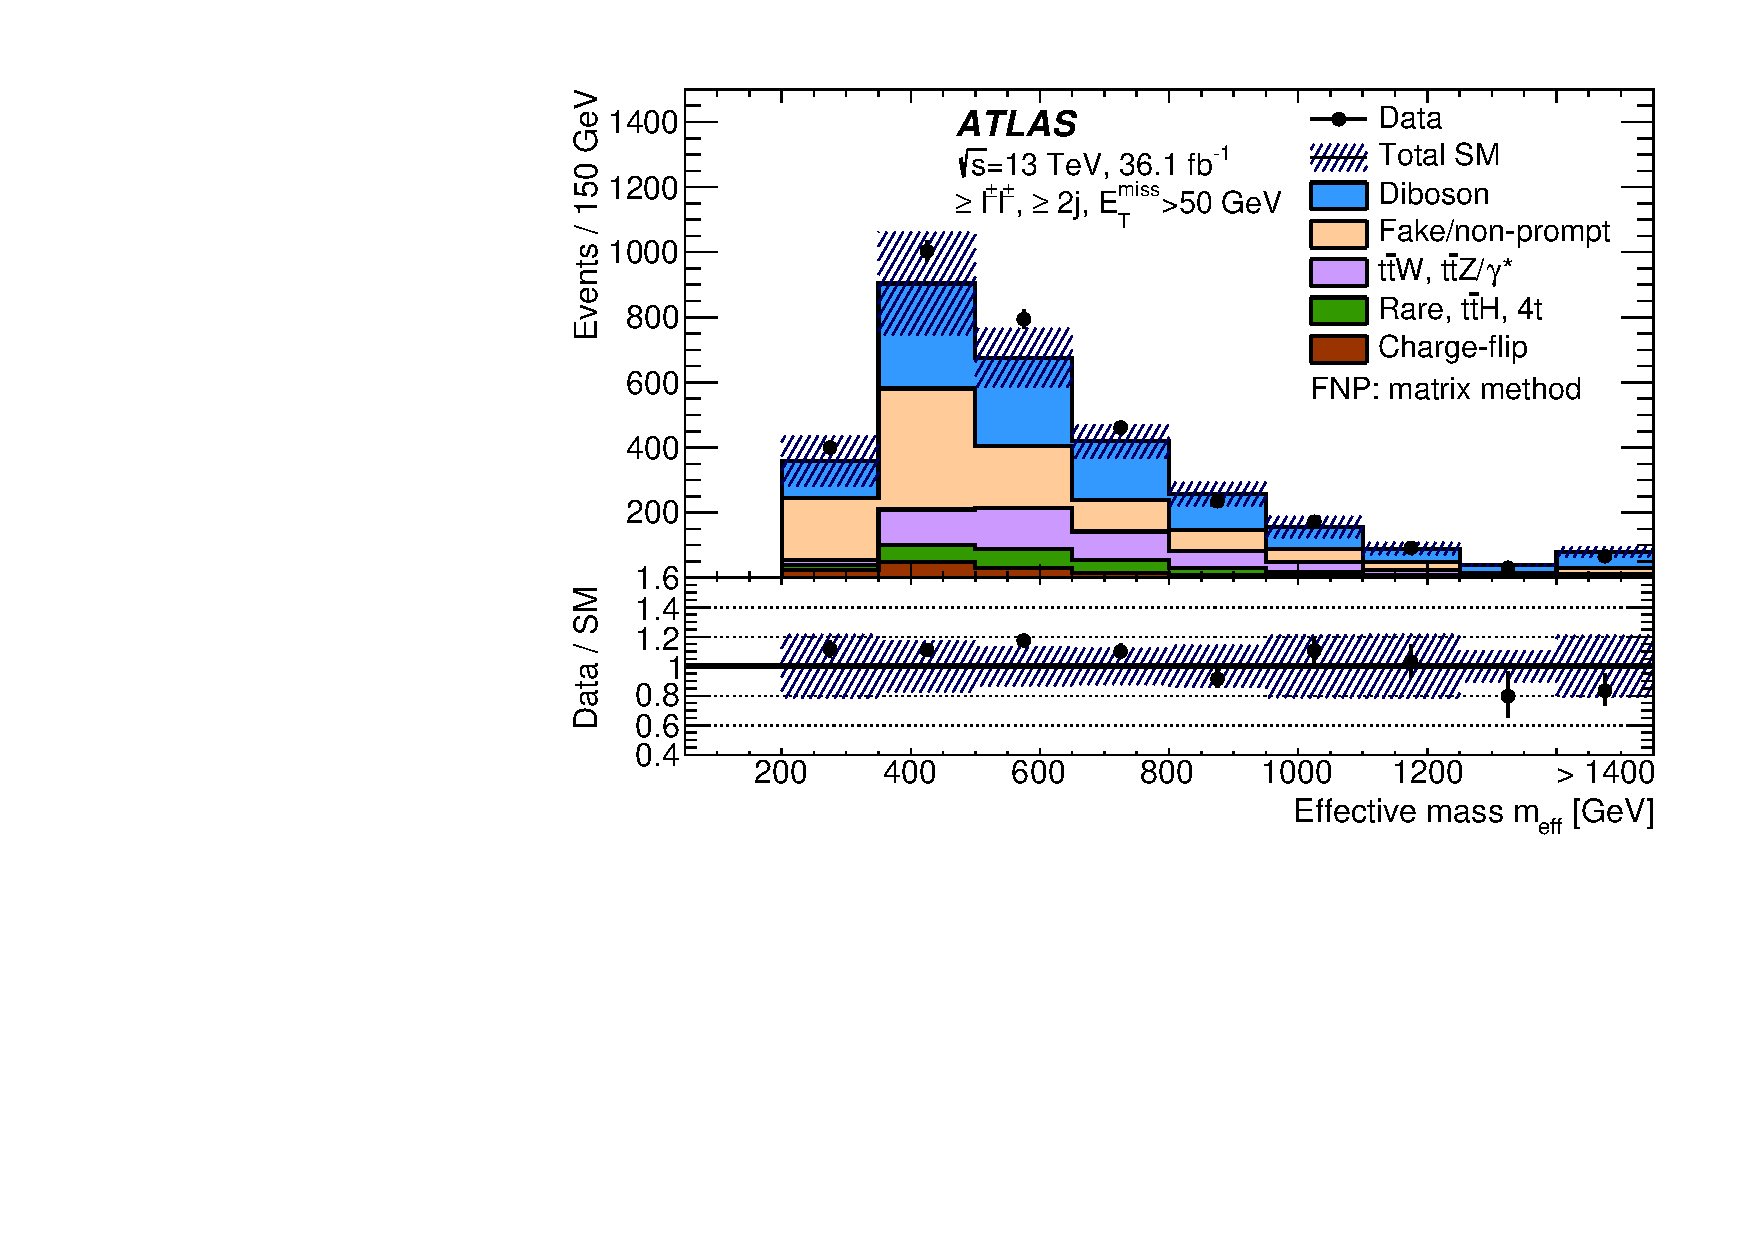
\includegraphics[width=\textwidth]{PAPER_DILEP_2JMET50_meff}\caption{}\label{fig:VRmeff1}\end{subfigure}
\begin{subfigure}[t]{0.49\textwidth}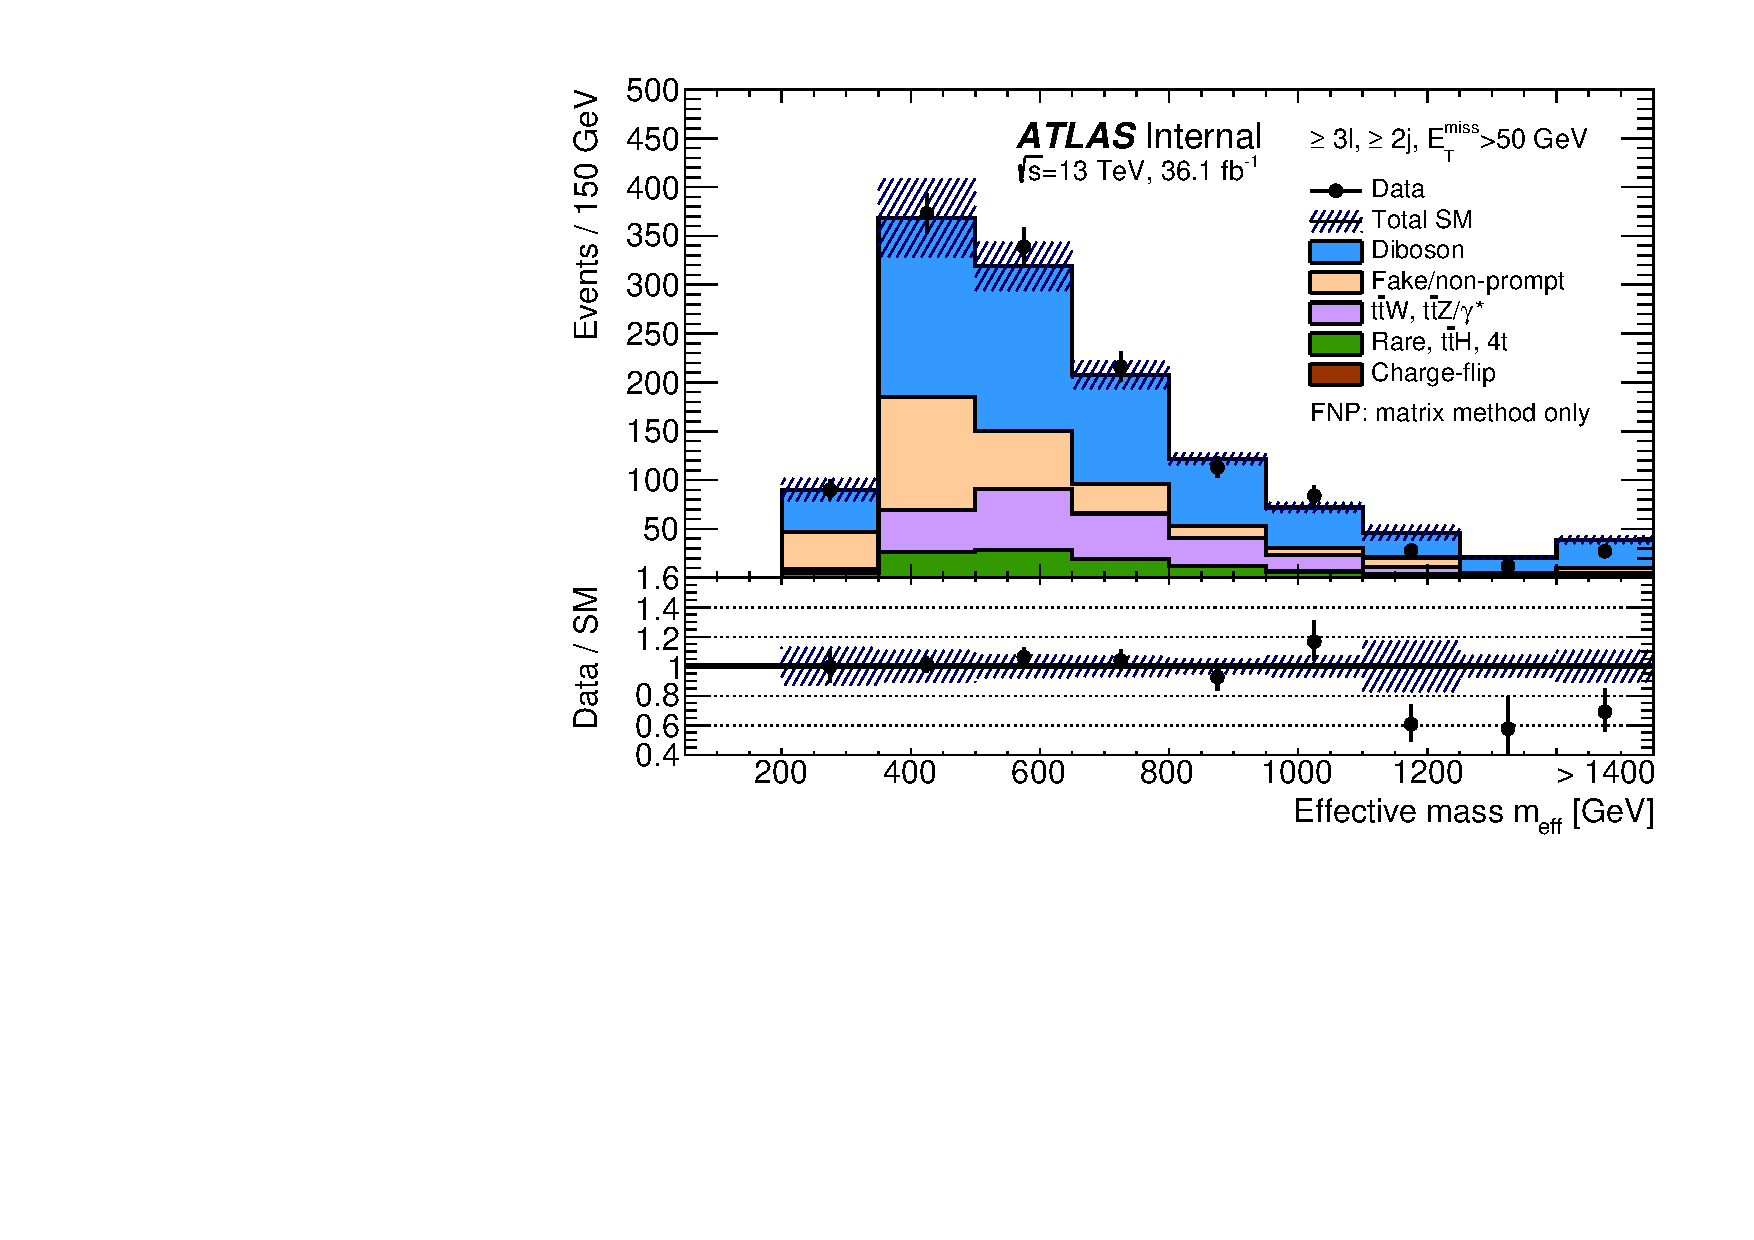
\includegraphics[width=\textwidth]{PAPER_TRILEP_2JMET50_meff}\caption{}\label{fig:VRmeff2}\end{subfigure}
\caption{
Distributions of (a) the number of jets, (b) the number of $b$-tagged jets and (c), (d) the effective mass. The distributions are made 
after requiring at least two jets ($\pT>40 \GeV$) and $\met>50 \GeV$, as well as at least two same-sign leptons ((a), (b), (c)) 
or three leptons (d). The uncertainty bands include the statistical uncertainties for the background prediction as well as the 
systematic uncertainties for fake- or non-prompt-lepton backgrounds (using the matrix method) and charge-flip electrons. Not included
are theoretical uncertainties in the irreducible background contributions.
The rare category is defined in the text.}
\label{fig:Bkg_distribs} 
\end{figure} 


\begin{figure}[htb!]
\begin{subfigure}[t]{0.49\textwidth}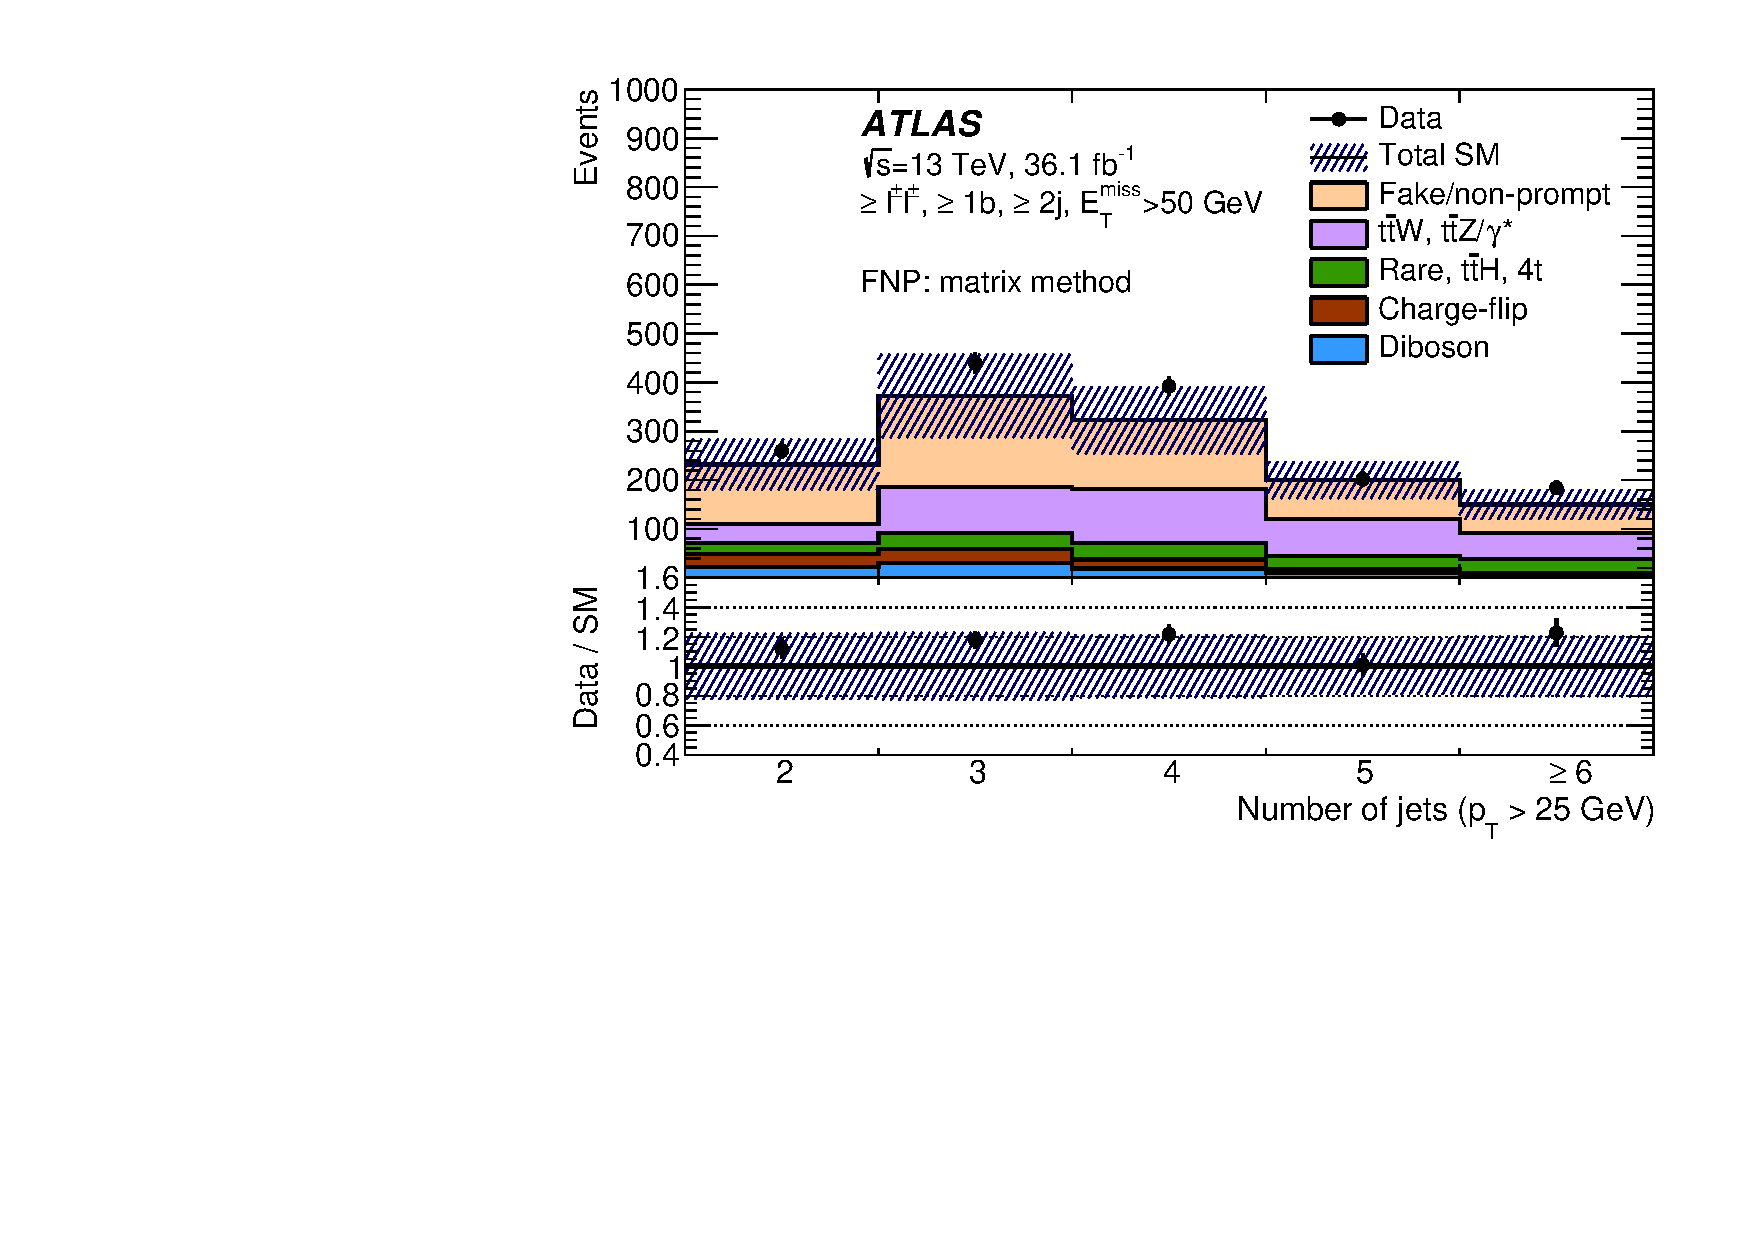
\includegraphics[width=\textwidth]{PAPER_DILEP_1B2JMET50_njets25_matrix}\caption{}\label{fig:VR1b2j_MxM}\end{subfigure}
\begin{subfigure}[t]{0.49\textwidth}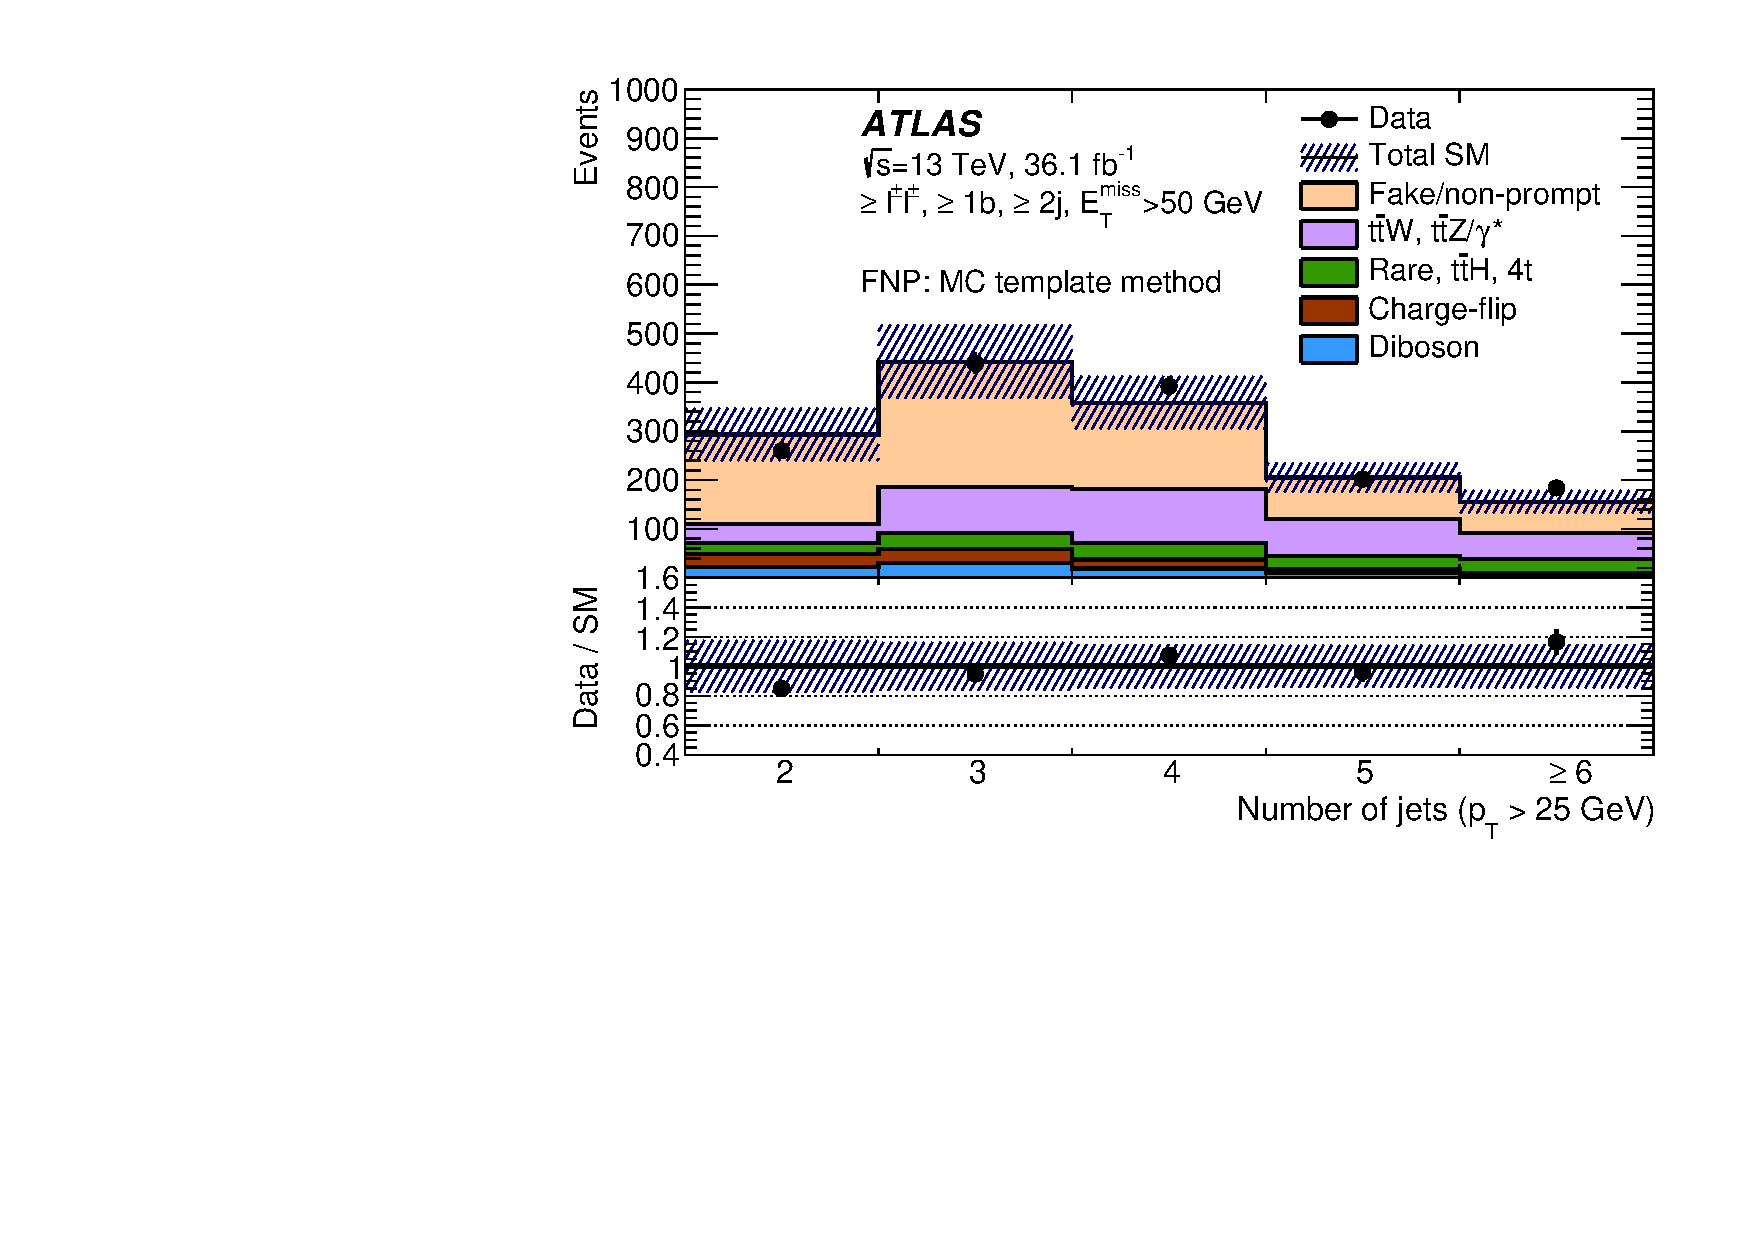
\includegraphics[width=\textwidth]{PAPER_DILEP_1B2JMET50_njets25_template}\caption{}\label{fig:VR1b2j_MCT}\end{subfigure}
\caption{
Distributions of the number of jets after requiring at least two jets ($\pT> 40 \GeV$) and $\met> 50 \GeV$, 
as well as at least two same-sign leptons. 
The fake or non-prompt leptons backgrounds are estimated alternatively with the matrix method (a) or the MC template method (b). 
The uncertainty band includes the statistical uncertainties for the background prediction as well as the
full systematic uncertainties for fake or non-prompt leptons backgrounds or charge-flip electrons. 
The rare category is defined in the text. In both figures, the last bin contains the overflow.
}
\label{fig:VR1b2j}
\end{figure}

\begin{figure}[htb!]
\centering
\begin{subfigure}[t]{0.66\textwidth}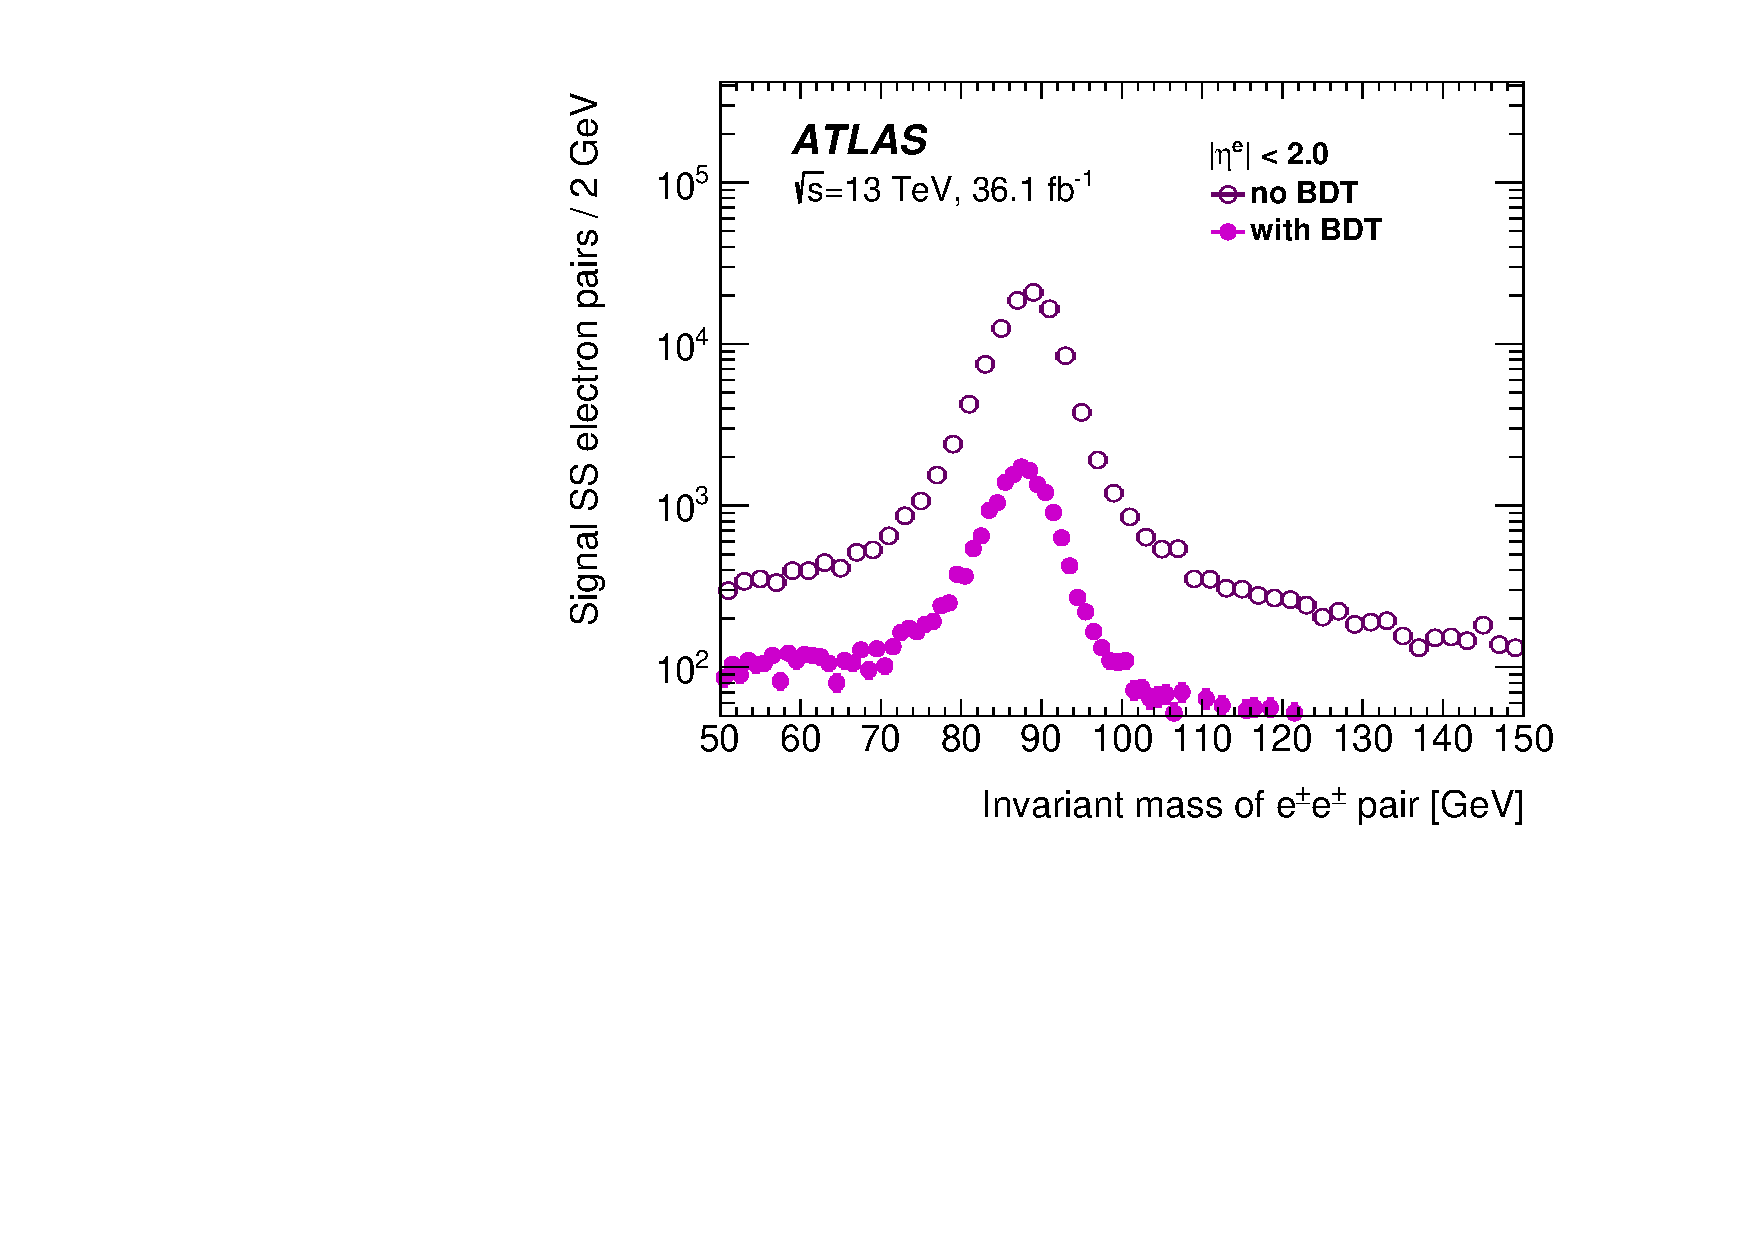
\includegraphics[width=\textwidth]{ETA_SS_BDTEL}\end{subfigure}
\caption{Invariant mass of the signal $e^{\pm} e^{\pm}$ pair distribution with (full markers) and without (open markers) charge-flip electron BDT selection applied.
}
\label{fig:ETA_SS_BDTEL}
\end{figure}
